\documentclass{article}


\usepackage[verbose=true,letterpaper]{geometry}
\usepackage[numbers]{natbib}


\usepackage[utf8]{inputenc} % allow utf-8 input
\usepackage[T1]{fontenc}    % use 8-bit T1 fonts
\usepackage{hyperref}       % hyperlinks
\usepackage{url}            % simple URL typesetting
\usepackage{booktabs}       % professional-quality tables
\usepackage{amsfonts}       % blackboard math symbols
\usepackage{nicefrac}       % compact symbols for 1/2, etc.
\usepackage{microtype}      % microtypography

\usepackage{amsmath,amsbsy,amssymb,amsfonts,amsthm}
\usepackage{bm}
\usepackage{graphicx}
\usepackage{subcaption}
\usepackage{xspace}
\usepackage{color}
\usepackage{algorithm, algpseudocode}
\usepackage{wrapfig}
\def\compactify{\itemsep=0pt \topsep=0pt \partopsep=0pt \parsep=0pt}

\usepackage{setspace}
\usepackage{enumitem}


\newtheorem{theorem}{Theorem}
\newtheorem{definition}[theorem]{Definition}
\newtheorem{assumption}[theorem]{Assumption}
\newtheorem{remark}[theorem]{Remark}
\newtheorem{claim}[theorem]{Claim}
\newtheorem{proposition}[theorem]{Proposition}
\newtheorem{lemma}[theorem]{Lemma}
\newtheorem{corollary}[theorem]{Corollary}

\newcommand{\E}{\mathbb{E}}
\newcommand{\Var}{\mathrm{Var}}
\newcommand{\mat}[1]{\bm{\mathit{#1}}}
\algdef{SE}[VARIABLES]{States}{EndStates}
   {\algorithmicvariables}
   {\algorithmicend\ \algorithmicvariables}
\algnewcommand{\algorithmicvariables}{\textbf{States}}
\algrenewcommand\Return{\State \algorithmicreturn{} }
\newcommand*{\AddNote}[4]{
    \begin{tikzpicture}[overlay, remember picture]
        \draw [decoration={brace,amplitude=0.5em},decorate,ultra thick,red]
            ($(#3)!(#1.north)!($(#3)-(0,1)$)$) --  
            ($(#3)!(#2.south)!($(#3)-(0,1)$)$)
                node [align=center, text width=2.5cm, pos=0.5, anchor=west] {#4};
    \end{tikzpicture}
}


\title{\tuner and the Art of Momentum Tuning}


\author{
  Jian Zhang, Ioannis Mitliagkas, Christopher R\'e \\
  Department of Computer Science\\
  Stanford University\\
  \texttt{\{zjian,imit,chrismre\}@cs.stanford.edu} \\
  %% examples of more authors
  %% \And
  %% Coauthor \\
  %% Affiliation \\
  %% Address \\
  %% \texttt{email} \\
  %% \AND
  %% Coauthor \\
  %% Affiliation \\
  %% Address \\
  %% \texttt{email} \\
  %% \And
  %% Coauthor \\
  %% Affiliation \\
  %% Address \\
  %% \texttt{email} \\
  %% \And
  %% Coauthor \\
  %% Affiliation \\
  %% Address \\
  %% \texttt{email} \\
}

\newcommand{\fix}{\marginpar{FIX}}
\newcommand{\new}{\marginpar{NEW}}

\newcommand{\tuner}{\textsc{YellowFin}\xspace}
\newcommand{\asynctuner}{closed-loop \textsc{YellowFin}\xspace}
\newcommand{\Asynctuner}{Closed-loop \textsc{YellowFin}\xspace}

\newcommand{\yell}[1]{#1}
\newcommand{\outline}[1]{}
\newcommand{\forjian}[1]{{\color{magenta}FOR JIAN: #1}}
\newcommand{\notes}[1]{{\color{green}NOTES: #1}}
\newcommand{\jianedits}[1]{#1}

\setlength{\parskip}{1.2ex}
\setlength{\parindent}{0pt}

\begin{document}

\maketitle

\begin{abstract}
\noindent Hyperparameter tuning is one of the big costs of deep learning. 
State-of-the-art optimizers, such as Adagrad, RMSProp and  Adam,
make things easier by adaptively tuning an individual learning rate for each variable.
This level of fine adaptation is understood to yield a more powerful method.
However, our experiments, as well as recent theory by \citet{wilson2017marginal}, 
show that hand-tuned stochastic gradient descent (SGD) achieves better results, at the same rate or faster.
The hypothesis put forth is that adaptive methods converge to different minima \cite{wilson2017marginal}.
Here we point out another factor: none of these methods tune their momentum parameter,
known to be very important for deep learning applications \cite{sutskever2013importance}.
Tuning the momentum parameter becomes even more important in asynchronous-parallel systems:
recent theory \cite{mitliagkas2016asynchrony} shows that asynchrony introduces momentum-like dynamics,
and that tuning down algorithmic momentum is important for efficient parallelization.  

We revisit the simple momentum SGD algorithm and show that hand-tuning a single learning rate and momentum value makes it competitive with Adam.
We then analyze its robustness in learning rate misspecification and objective curvature variation.
Based on these insights, we design \tuner, an automatic tuner for both momentum and learning rate in SGD.
\tuner optionally uses a novel momentum-sensing component along with a negative-feedback loop mechanism to compensate for the added dynamics of asynchrony on the fly.
We empirically show \tuner converges in fewer iterations than Adam on large ResNet and LSTM models,
	with a speedup up to $2.8$x in synchronous and $2.7$x in asynchronous settings.% on ResNet and LSTM models.
\end{abstract}





\section{Introduction}


\outline{[Problem.]}
Accelerated forms of stochastic gradient descent (SGD), pioneered by
\citet{polyak1964some} and \citet{nesterov1983method}, are the de-facto
training algorithms for deep learning.
Their use requires a sane choice for their {\em hyperparameters}: 
typically a {\em learning rate} and {\em momentum parameter} \citep{sutskever2013importance}.
However, tuning hyperparameters is arguably the most time-consuming part of deep learning, with thousands of productive hours sacrificed and many papers outlining best tuning practices written
\cite{bengio2012practical,orr2003neural,bengio2012deep,bottou2012stochastic}.

\outline{[previous approach]}
Deep learning researchers have proposed a number of methods to deal with hyperparameter optimization. 
Na\"ive methods, like the grid-search,
are prohibitively expensive for all but the smallest problems. 
Smart black-box methods \cite{bergstra2012random,snoek2012practical}
do not explicitly take into account the problem specifics and spend time testing multiple configurations.
Adaptive methods provide an attractive alternative.
They aim to tune a single run on the fly and have been largely successful in relieving practitioners of tuning the learning rate. 
Algorithms like Adagrad \cite{duchi2011adaptive}, RMSProp \cite{tieleman2012lecture} and Adam \cite{kingma2014adam} use the magnitude of gradient elements to tune learning rates {\em individually for each variable}.
\yell{
This increased flexibility sounds great,
however our experiments and recent analysis in literature \cite{wilson2017marginal} suggest that methods that adapt multiple learning rates, yield marginal benefits compared to momentum SGD.
\citet{wilson2017marginal} argue that those methods also have worse generalization.
We make another argument: adaptive methods also suffer because they do not tune their momentum parameter.
}

Momentum is a fundamental parameter at the heart of accelerated optimization,
lending its name to the most ubiquitous accelerated method \cite{polyak1964some}, commonly referred to as {\em momentum}.
Classic \cite{polyak1964some} and recent results \cite{sutskever2013importance} alike show that proper momentum tuning has a significant impact on training speed. 
Momentum becomes even more critical on distributed systems. 
Recently, \citet{mitliagkas2016asynchrony} showed that, in asynchronous-parallel systems---a popular design for efficient distributed training without synchronization 
\cite{recht2011hogwild,dean2012large,chilimbi2014project,hadjis2016omnivore}---the system introduces momentum-like dynamics into the optimization.
As a result,
one should reduce the amount of algorithmic momentum to get fast convergence~\cite{hadjis2016omnivore}.
As part of a collaboration with an industry affiliate and a big research lab, we were able to verify that tuning momentum improves convergence on thousand-node scales.
However, grid-searching momentum on very large cluster jobs becomes especially challenging.
Better understanding of momentum and its rich properties is interesting in its own right and could yield a next generation of adaptive methods that perform {\em automatic momentum tuning}. 




\begin{wrapfigure}[13]{R}{0.47\textwidth}
\vspace{-2.0em}
\begin{minipage}{1.0\linewidth}
\begin{figure}[H]
	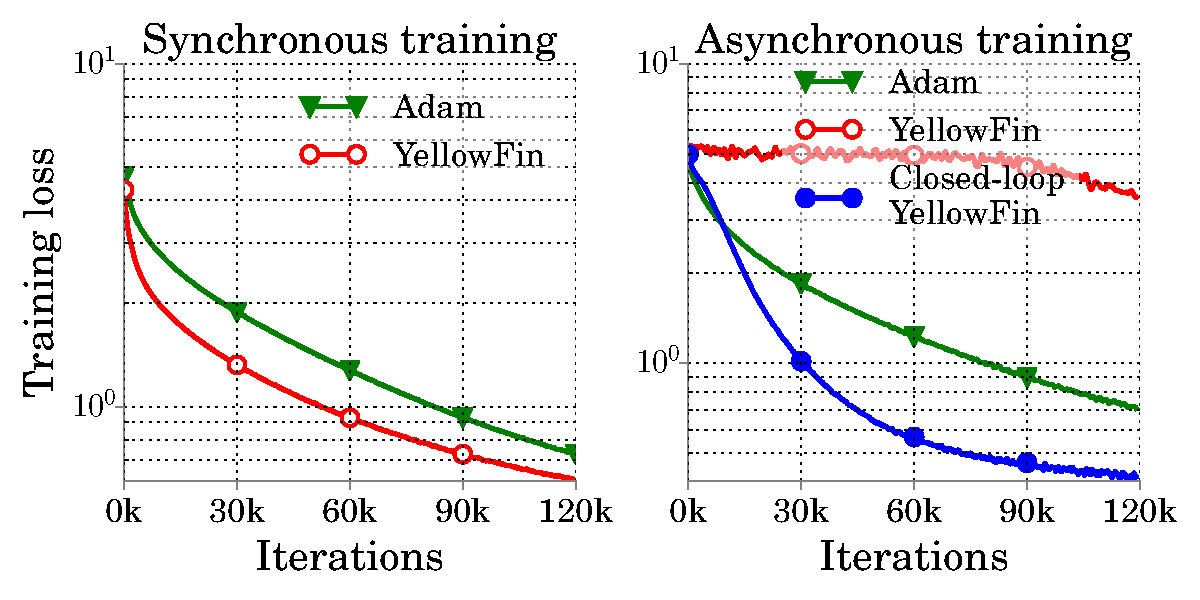
\includegraphics[width=1.\linewidth]{experiment_results/spotlight.pdf}
	\caption{\tuner in comparison to Adam on a ResNet (CIFAR100, cf.\ Section~\ref{sec:experiments}).	
	}
\end{figure}
\end{minipage}
\end{wrapfigure}
We revisit the basic SGD update that uses Polyak's momentum and a single learning rate for all variables.
We empirically show that, when hand-tuned, momentum SGD achieves faster convergence than Adam for a large class of models.
We then formulate the optimization update as a dynamical system and study certain robustness properties of the momentum operator.
Building on our analysis, we design \tuner, an automatic hyperparameter tuner for momentum SGD.
\tuner tunes the learning rate and momentum on the fly, and uses a novel {\em closed-loop control architecture} to compensate for the added dynamics of asynchrony.
Specifically:
\begin{itemize}[leftmargin=2em]
\setlength\itemsep{0.2em}
\item
Our analysis in Section~\ref{sec:momentum_operator} shows that momentum is robust to learning rate misspecification and curvature variation,
two desirable properties for deep learning.
These properties stem from a known but obscure fact:
the momentum operator's spectral radius is constant in a large subset of the hyperparameter space.
\item
In Section~\ref{sec:sync_tuner}, we use these robustness insights and a simple quadratic model analysis to design \tuner, an automatic tuner for momentum SGD.
\tuner uses on-the-fly measurements from the gradients of the system to tune both learning rate and momentum.
\item In Section~\ref{sec:async_tuner} we present \asynctuner, suited for asynchronous training.
It measures the total momentum in a running system, including any asynchrony-induced momentum. 
This measurement is used in a negative feedback loop to control the value of algorithmic momentum.% on the fly.

\end{itemize}





\outline{[empirical performance statement on \tuner]}
In Section~\ref{sec:experiments}, we demonstrate empirically that \yell{on ResNets and LSTMs}
\tuner  converges in fewer iterations compared to:
(i) hand-tuned momentum SGD (a speedup of up to 2.2x);
and (ii) hand-tuned Adam (up to 2.8x speedup).
Under asynchrony, we demonstrate that state-of-the-art adaptive methods suffer due to lack of momentum tuning.
In the same setting, the closed-loop control architecture speeds up \tuner by up to 2x, 
making it at least 2.7x faster than Adam.
We conclude with related work in Section~\ref{sec:related} and discussion in Section~\ref{sec:discussion}.
We release a TensorFlow implementation of \tuner, that can be used as drop-in replacement for any optimizer\footnote{Our TensorFlow implementation can be accessed at \url{https://github.com/JianGoForIt/YellowFin}.}.
We are also planning a PyTorch release.




\section{The momentum operator}
\label{sec:momentum_operator}

\newcommand{\gc}{generalized curvature\xspace}
\newcommand{\Gc}{Generalized curvature\xspace}

In this section we identify the main technical insights that guide the design of \tuner. 
We first establish some preliminaries on momentum gradient descent 
and then perform a simple dynamical analysis.
We show that momentum is robust to learning rate misspecification and curvature variation for a class of non-convex objectives, two important properties for deep learning.



\subsection{Preliminaries}
\label{sec:robust_preliminaries}
We aim to minimize some objective $f(x)$.
In machine learning, $x$ is referred to as {\em the model} and the objective is some {\em loss function}.
A low loss implies a well-fit model.
Gradient descent-based procedures use the gradient of the objective function, $\nabla f(x)$, to update the model iteratively.
Polyak's momentum gradient descent update \citep{polyak1964some} is given by
\begin{align}
	x_{t+1}  &= x_t - \alpha \nabla f(x_t) + \mu (x_t - x_{t-1}),
	\label{eqn:momentum_gd}
\end{align} 
where $\alpha$ denotes the learning rate and $\mu$ the value of momentum used.
Momentum's main appeal is its established ability to {\em accelerate convergence} \cite{polyak1964some}. 
On a strongly convex smooth function with condition number $\kappa$, the optimal convergence rate of gradient descent ($\mu=0$)
 is $O(\frac{\kappa-1}{\kappa+1})$~\cite{nesterov2013introductory}.
\yell{On the other hand, for certain classes of strongly convex and smooth functions, like quadratics,  the optimal momentum value,
\begin{equation}
	\mu^* = \left(\frac{\sqrt{\kappa}-1}{\sqrt{\kappa}+1}\right)^2,
	\label{eqn:optimal_momentum}
\end{equation}
yields the optimal accelerated rate $O(\frac{\sqrt{\kappa}-1}{\sqrt{\kappa}+1})$}.\footnote{
\yell{
This guarantee does not generalize to arbitrary strongly convex functions \cite{lessard2016analysis}.
Nonetheless, acceleration is typically observable in practice (cf. Section~\ref{sec:robust_properties}).
}
}
This is the smallest value of momentum that {\bf ensures the same rate of convergence along all directions}.
This fact is often hidden away in proofs. 
We shed light on some of its previously unknown implications in Section~\ref{sec:robust_properties}. % and use them in our tuner in Section~\ref{sec:sync_tuner}.



\subsection{Robustness properties of the momentum operator}
\label{sec:robust_properties}
In this section we analyze the dynamics of momentum on a simple class of one dimensional, non-convex objectives.
We first introduce the notion of {\em generalized curvature} and use it to describe the momentum operator.
Then we discuss some properties of the momentum operator.


\begin{definition}[\Gc]
\label{def:generalized_curvature}
The derivative of $f(x):\mathbb{R}\rightarrow\mathbb{R}$, can be written as 
\begin{equation}
	 f'(x) = h(x) (x - x^*) 
	\label{eqn:generalized_curvature}
\end{equation}
for some $h(x) \in \mathbb{R}$, where $x^*$ is the global minimum of $f(x)$.
We call $h(x)$ the {\em generalized curvature}.
\end{definition}

The \gc describes, in some sense, curvature with respect to the optimum,  $x^*$.
For quadratic objectives, it coincides with the standard definition of curvature.
It is the sole quantity related to the objective that influences the dynamics of gradient descent.
For example, the contraction of a gradient descent step is $1-\alpha h(x_t)$.
Let $\mat{A}_t$ denote the {\em momentum operator} at time $t$.
Using a state-space augmentation, we can express the momentum update as
\begin{align}
{\begin{pmatrix}
x_{t+1} - x^*\\
x_t - x^* \\
\end{pmatrix}}
=
{\begin{bmatrix}
1-\alpha h(x_t) + \mu & - \mu \\
1 & 0 \\
\end{bmatrix}}
{\begin{pmatrix}
x_t - x^* \\
x_{t-1} - x^*\\
\end{pmatrix}}
\triangleq
\mat{A}_t
{\begin{pmatrix}
x_t - x^* \\
x_{t-1} - x^*\\
\end{pmatrix}}.
\label{equ:one_dim_22_rec}
\end{align}

\begin{lemma}[Robustness of the momentum operator]
\label{lem:robustness}
If the generalized curvature, $h$, and hyperparameters $\alpha,\mu$ are in the {\em robust region}, that is: 
\begin{align}
{(1-\sqrt{\mu})^2} &\leq \alpha h(x_t) \leq {(1+\sqrt{\mu})^2},
\label{eqn:robust_region}
\end{align}
then the spectral radius of the momentum operator only depends on  momentum: $	\rho(\mat{A}_t) = \sqrt{\mu}
$. 
\end{lemma}
We can explain Lemma~\ref{lem:robustness} as robustness with respect to learning rate and to variations in curvature.



\begin{wrapfigure}[15]{R}{0.3\textwidth}
\vspace{-2.5em}
\begin{minipage}{1.0\linewidth}
\begin{figure}[H]
  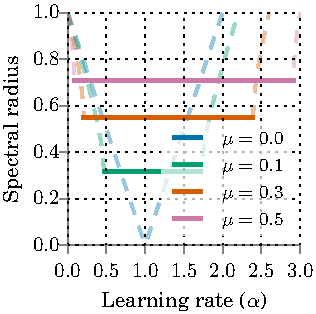
\includegraphics[width=1.0\linewidth]{figures/spectral_radii}
\caption{
Spectral radius of momentum operator on scalar quadratic.
}
\label{fig:lr_robustness}
\end{figure}
\end{minipage}
\end{wrapfigure}
\paragraph{Momentum is robust to learning rate misspecification}
\label{sec:lr_robustness}
For a one dimensional strongly convex quadratic objective,
we get $h(x)=h$ for all $x$ and Lemma~\ref{lem:robustness} suggests that $\rho(\mat{A}_t)=\sqrt{\mu}$ as long as
\begin{align}
{(1-\sqrt{\mu})^2/h} &\leq \alpha \leq {(1+\sqrt{\mu})^2/h}.
\label{eqn:lr_robustness}
\end{align}

In Figure~\ref{fig:lr_robustness}, we plot $\rho(\mat{A}_t)$ for different $\alpha$ and $\mu$.
As we increase the value of momentum, the optimal rate of convergence $\sqrt{\mu}$ is achieved by an ever-widening range of learning rates. 
Furthermore, for objectives with large condition number, higher values of momentum are {\em both faster and more robust}.
{\bf This property influences the design of our tuner:} as long as the learning rate satisfies \eqref{eqn:lr_robustness}, we are in the {\em robust region} and 
expect the same asymptotics. For example a convergence rate of $\sqrt{\mu}$ for quadratics, independent of the learning rate.
Having established that, we can just focus on optimally tuning momentum.




\paragraph{Momentum is robust to curvature variation}
\label{sec:curvature_robustness}

As discussed in Section~\ref{sec:robust_preliminaries}, the intuition hidden in classic results
is that for strongly convex smooth objectives, the momentum value in \eqref{eqn:optimal_momentum} guarantees the same rate of convergence along all directions. 
We extend this intuition to certain non-convex functions.
Lemma~\ref{lem:robustness} guarantees a constant, time-homogeneous spectral radius for the momentum operators $(\mat{A}_t)_t$ if 
\eqref{eqn:robust_region} is satisfied at every step. 
This motivates an extension of the condition number.
\begin{definition}[Generalized condition number]
We define the generalized condition number (GCN) of a scalar function, $f(x):\mathbb{R}\rightarrow \mathbb{R}$, to be the dynamic range of its generalized curvature, $h(x)$:
\begin{equation}
	\nu = \frac{\sup_{x \in dom(f)} h(x)}{ \inf_{x \in dom(f)} h(x)}
\end{equation}
\end{definition}
The GCN captures variations in generalized curvature along a scalar slice.
From Lemma~\ref{lem:robustness} we get
\begin{equation}
	\mu^* = \left(\frac{\sqrt{\nu}-1}{\sqrt{\nu}+1}\right)^2,
	\quad
	\alpha^* = \frac{(1-\sqrt{\mu})^2}{\inf_{x \in dom(f)}h(x)}
	\label{eqn:noiseless_tuning_rule}
\end{equation}
as the optimal hyperparameters. 
Specifically, $\mu^*$ is the smallest momentum value that guarantees a homogeneous spectral radius of $\sqrt{\mu^*}$ for all $(\mat{A}_t)_t$.
The spectral radius of an operator describes its asymptotic behavior. 
However, the product of a sequence of operators $\mat{A}_t\cdots\mat{A}_1$ all with spectral radius $\sqrt{\mu}$ does not necessarily follow the asymptotics of $\sqrt{\mu}^t$.
In other words, {\em we do not provide a convergence rate guarantee}.
Instead, we provide empirical evidence in support of this intuition. 


For example, the non-convex objective in Figure~\ref{fig:curvature_robustness}(a),
composed of two quadratics with curvatures $1$ and $1000$, has a GCN of $1000$.
Using the tuning rule of \eqref{eqn:noiseless_tuning_rule}, and running the momentum algorithm (Figure~\ref{fig:curvature_robustness}(b)) yields a practically constant rate of convergence throughout.
In Figures~\ref{fig:curvature_robustness}(c,d) we demonstrate that for an LSTM,
the majority of variables follows a $\sqrt{\mu}$ convergence rate.
\textbf{This property influences the design of our tuner:}
in the next section we use the tuning rules of \eqref{eqn:noiseless_tuning_rule} in \tuner,
generalized appropriately to handle SGD noise.






\begin{figure}[t]
\centering
\begin{tabular}{c c c c}
  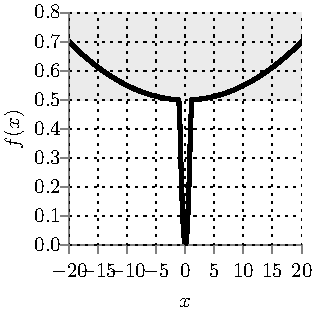
\includegraphics[width=0.23\linewidth]{figures/non_convex_toy} &
  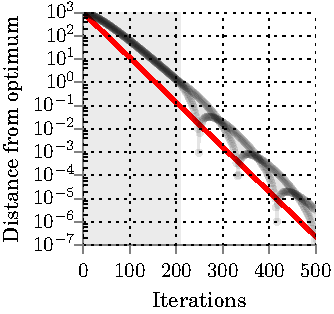
\includegraphics[width=0.24\linewidth]{figures/non_convex_constant_rate} &
  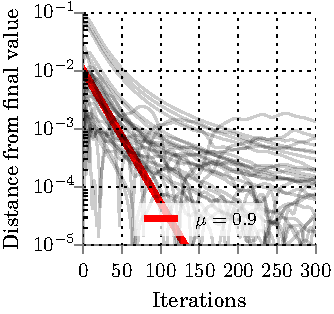
\includegraphics[width=0.24\linewidth]{figures/constant_rate_09} &
  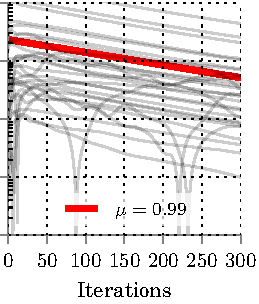
\includegraphics[width=0.19\linewidth]{figures/constant_rate_099} \\
  (a) & (b) & (c) &(d)
\end{tabular}
\caption{(a) Non-convex toy example;
(b) constant convergence rate achieved empirically on the objective of (a) tuned according to \eqref{eqn:noiseless_tuning_rule};
(c,d)
LSTM on MNIST: as momentum increases, more variables (shown in grey) fall in the robust region and follow the robust rate, $\sqrt{\mu}$.}
\label{fig:curvature_robustness}
\end{figure}











\vspace{-0.2em}
\section{The \tuner tuner}
\label{sec:sync_tuner}
\vspace{-0.2em}
%In this section we describe \tuner, our tuner for momentum SGD.
%We introduce a noisy quadratic model and work on a local quadratic approximation of $f(x)$ to apply the tuning rule of \eqref{eqn:noiseless_tuning_rule} to SGD on an arbitrary objective.
%\tuner is our implementation of that rule.

Here we describe our tuner for momentum SGD that uses the same learning rate for all variables.
We first introduce a noisy quadratic model $f(x)$ as the local approximation of an arbitrary one-dimensional objective. On this approximation, we extend the tuning rule of \eqref{eqn:noiseless_tuning_rule} to SGD. In section~\ref{sec:tuner}, \emph{we generalize the discussion to multidimensional objectives; it yields the \tuner tuning rule}.


\paragraph{Noisy quadratic model}
\label{sec:noisy_quadratics}

\newcommand{\oac}{origin-adjusted curvature }
\newcommand{\bx}{\bar{x}}


We consider a scalar quadratic 
\begin{equation}
	f(x) = \frac{h}{2} x^2 + C 
	= \sum_i \frac{h}{2n}(x-c_i)^2
	\triangleq \frac{1}{n} \sum_i f_i(x)
%	\quad \sum_i c_i = 0.
	\label{eqn:noise_quad_1d}
\end{equation}
with $\sum_i c_i = 0$. $f(x)$ is a quadratic approximation of the original objectives with $h$ and $C$ derived from measurement on the original objective. The function $f(x)$ is defined as the average of $n$ {\em component functions}, $f_i$.
This is a common model for SGD, where we use only a single data point (or a mini-batch) drawn uniformly at random, $S_t \sim \mathrm{Uni}([n])$ to compute a noisy gradient, $\nabla f_{S_t}(x)$, for step $t$.
Here, $C=\frac{1}{2n}\sum_i h c_i^2$ denotes the {\em gradient variance}.
As optimization on quadratics decomposes into scalar problems along the principal eigenvectors of the Hessian, the scalar model in~\eqref{eqn:noise_quad_1d} is sufficient to study local quadratic approximations of multidimensional objectives.
Next we get an {\em exact} expression for the mean square error after running momentum SGD on the scalar quadratic in~\eqref{eqn:noise_quad_1d} for $t$ steps.



\begin{lemma}
\label{lem:main_lemma}
Let $f(x)$ be defined as in \eqref{eqn:noise_quad_1d},
$x_1=x_0$ and $x_t$ follow the momentum update \eqref{eqn:momentum_gd} with stochastic gradients $\nabla f_{S_t}(x_{t-1})$ for $t \geq 2$.
Let $\mat{e}_1=[1, 0]^T$, the expectation of squared distance to the optimum $x^*$ is
	\begin{equation}
	\begin{aligned}
		\E (x_{t+1} - x^{*})^2 & = (\mat{e}^{\top}_1 \mat{A}^t [x_1 - x^{*}, x_0-x^{*}]^{\top})^2 \\
		& + \alpha^2 C \mat{e}^{\top}_1 (\mat{I} - \mat{B}^t)(\mat{I} - \mat{B})^{-1}\mat{e}_1	,
		\label{equ:squared_dist_exact}	
	\end{aligned}
	\end{equation}
where the first and second term correspond to squared bias 
and variance, and their corresponding momentum dynamics are captured by operators
	\begin{equation}
	\begin{gathered}
		\mat{A} = \begin{bmatrix}
		1-\alpha h + \mu & - \mu\\
		1 & 0 \\
		\end{bmatrix}, \\
%		\quad
		\mat{B} = 
		\begin{bmatrix}
		(1-\alpha h + \mu)^2 &  \mu^2 & -2\mu(1-\alpha h + \mu)\\
		1 & 0 & 0 \\
		1-\alpha h + \mu & 0 & - \mu
		\end{bmatrix}.
		\label{equ:mat_def}
	\end{gathered}
	\end{equation}
\end{lemma}

\yell{
Even though it is possible to numerically work on~\eqref{equ:squared_dist_exact} directly,
we use a scalar, asymptotic surrogate in~\eqref{eqn:asymptotic_surrogate} based on the spectral radii of operators to simplify analysis and expose insights.
This decision is supported by our findings in Section~\ref{sec:momentum_operator}: the spectral radii can capture empirical convergence rate.}
\begin{equation}
\begin{aligned}
%	\E ( x_{t+1} - x^{*} )^2
%	\approx  \rho(\mat{A})^{2t} ( x_0 - x_{*} )^2 
%		+ (1-\rho(\mat{B})^{t}) \frac{\alpha^2 C}{1-\rho(\mat{B})}
	&\E ( x_{t+1} - x^{*} )^2 \\
	\approx & \rho(\mat{A})^{2t} ( x_0 - x_{*} )^2 
		+ (1-\rho(\mat{B})^{t}) \frac{\alpha^2 C}{1-\rho(\mat{B})}
	\label{eqn:asymptotic_surrogate}
\end{aligned}
\end{equation}

One of our design decisions for \tuner 
is to always work in the robust region of Lemma~\ref{lem:robustness}.
We know that this implies a spectral radius $\sqrt{\mu}$ of the momentum operator, $\mat{A}$, for the bias. 
Lemma~\ref{lem:spectral_var_control} shows that under the exact same condition, the variance operator $\mat{B}$ has spectral radius $\mu$.
 

\begin{lemma}
\label{lem:spectral_var_control}
The spectral radius of the variance operator, $\mat{B}$ is $\mu$, if ${(1-\sqrt{\mu})^2} \leq  \alpha h \leq {(1+\sqrt{\mu})^2}$.
\end{lemma}

As a result, the surrogate objective of \eqref{eqn:asymptotic_surrogate}, takes the following form in the robust region.  
\begin{equation}
	\E ( x_{t+1} - x^{*} )^2 
	\approx \mu^t ( x_0 - x^{*} )^2
		+ (1-\mu^t) \frac{\alpha^2 C}{1-\mu}
	\label{eqn:noisy_square_dist}
\end{equation}
We extend this surrogate to multidimensional cases to extract a noisy tuning rule for \tuner.

%\vspace{-0.25em}
\subsection{Tuning rule}
\label{sec:tuner}
\vspace{-0.25em}

In this section, we present \textsc{SingleStep}, the tuning rule of YellowFin (Algorithm~\ref{alg:basic-algo}). Based on the surrogate in~\eqref{eqn:noisy_square_dist}, \textsc{SingleStep} is a multidimensional SGD version of the noiseless tuning rule in~\eqref{eqn:noiseless_tuning_rule}. We first generalize~\eqref{eqn:noiseless_tuning_rule} and~\eqref{eqn:noisy_square_dist} to multidimensional cases, and then discuss \textsc{SingleStep}.% in details.

As discussed in Section~\ref{sec:robust_properties}, GCN $\nu$ captures the dynamic range of generalized curvatures in a one-dimensional objective with varying curvature. The consequent robust region described by~\eqref{eqn:noiseless_tuning_rule} implies homogeneous spectral radii. 
%\emph{In multidimensional cases, we use a single learning rate and momentum for the entire model.} 
On a multidimensional non-convex objective, each one-dimensional slice passing a minimum $x^*$ can have \emph{varying curvature}. As we use \emph{a single $\mu$ and $\alpha$ for the entire model}, if $\nu$ simultaneously captures the dynamic range of generalized curvature over all these slices, $\mu$ and $\alpha$ in~\eqref{eqn:noiseless_tuning_rule} are in the robust region for all these slices. This implies homogeneous spectral radii $\sqrt{\mu}$ according to Lemma~\ref{lem:robustness}, empirically facilitating convergence at a common rate along all the directions. 

Given homogeneous spectral radii $\sqrt{\mu}$ along all directions, the surrogate in~\eqref{eqn:noisy_square_dist} generalizes on the local quadratic approximation of multiple dimensional objectives. On this approximation with minimum $x^*$, the expectation of squared distance to $x^*$, $\E \| x_0 - x^*\|^2$, decomposes into independent scalar components along the eigenvectors of the Hessian. We define gradient variance $C$ as the sum of gradient variance along these eigenvectors. The one-dimensional surrogates in~\eqref{eqn:noisy_square_dist} for the independent components sum to $\mu^t\| x_0 - x^* \|^2 + (1-\mu^t)\alpha^2 C / (1 - \mu)$, the \emph{multidimensional surrogate} corresponding to the one in~\eqref{eqn:noisy_square_dist}. 
%Given homogeneous spectral radii $\sqrt{\mu}$ along all directions, the surrogate in~\eqref{eqn:noisy_square_dist} generalizes via multidimensional local quadratic approximations. Assuming the quadratic approximation aligns with standard axes, the expectation of squared distance to the optimum of the approximation, $\E\|x_t - x^*\|^2$, decomposes along the standard axes. As the initial squared distance $\| x_0 - x^*\|^2$ and gradient variance $C$ also decompose along the axes, the one dimensional surrogates along axes sums to $\mu^t\| x_0 - x^* \|^2 + (1-\mu^t)\alpha^2 C / (1 - \mu)$, the surrogates corresponding to the one in~\eqref{eqn:noisy_square_dist}. 
%	Note for quadratic approximation not aligned with the axes, this \emph{multidimensional surrogates} is attained by decomposing along eigenvectors of the quadratic approximation's Hessian, instead of standard axes. 

%%\begin{minipage}{0.5\linewidth}
%%\vspace{-0.25em}
%\begin{equation}
%\begin{aligned}
%	\textsc{(SingleStep)} \notag \\
%	 \mu_t, \alpha_t & = && \arg \min_{\mu} \mu D^2
%		+ \alpha^2 C \\
%	s.t. & &&\mu \geq \left(\frac{\sqrt{h_{\max}/h_{\min} }-1}{\sqrt{h_{\max}/h_{\min}}+1}\right)^2 \\
%	& &&\alpha = \frac{(1-\sqrt{\mu})^2}{h_{\min}}
%\end{aligned}
%\label{equ:noisy_min}
%\end{equation}
%%\end{minipage}
%\begin{minipage}{0.025\linewidth}
%\ 
%\end{minipage}
%\begin{minipage}{0.45\linewidth}
%\vspace{-1.5em}
%\begin{algorithm}[H]
%	\footnotesize
%	\caption{\jianedits{\tuner}}
%	\begin{algorithmic}
%	\State \textbf{state: } $\alpha \gets 1.0$, $\mu \gets 0.0$%, $w\gets20$
%	\Function{\tuner}{$\text{gradient } g_t$, $\beta$}
%	\State $h_{\max}, h_{\min} \gets \Call{CurvatureRange}{g_t, \beta}$
%	\State $C \gets \Call{Variance}{g_t, \beta}$ 
%	\State $D \gets \Call{Distance}{g_t, \beta}$ 
%
%	\State $\mu_t, \alpha_t \gets \Call{SingleStep}{C, D, h_{\max}, h_{\min}}$
%	\State $\mu \gets \beta \cdot \mu + (1 - \beta) \cdot \mu_t$
%	\State $\alpha \gets \beta \cdot \alpha + (1 - \beta) \cdot \alpha_t$ %\Comment{Smoothing learning rate and momentum for stable control}
%	\Return $\mu, \alpha$
%	\EndFunction
%	\end{algorithmic}
%	\label{alg:basic-algo}
%\end{algorithm}
%\end{minipage}
%%%%%%%%%%%%%%%%%%%%%%%%% new algorithm %%%%%%%%%%%%%%%%%%%%%%%%
%%\begin{minipage}{0.475\linewidth}
%%\vspace{-0.25em}
%\begin{algorithm}[H]
%	\footnotesize
%	\caption{\jianedits{\tuner}}
%	\begin{algorithmic}
%%	\State \textbf{state: } $\alpha \gets 1.0$, $\mu \gets 0.0$%, $w\gets20$
%	\Function{\tuner}{$\text{gradient } g_t$, $\beta$}
%	\State $h_{\max}, h_{\min} \gets \Call{CurvatureRange}{g_t, \beta}$
%	\State $C \gets \Call{Variance}{g_t, \beta}$ 
%	\State $D \gets \Call{Distance}{g_t, \beta}$ 
%
%	\State $\mu_t, \alpha_t \gets \Call{SingleStep}{C, D, h_{\max}, h_{\min}}$
%%	\State $\mu_t, \alpha_t \gets \Call{SingleStep}{C, D, h_{\max}, h_{\min}}$
%%	\State $\mu \gets \beta \cdot \mu + (1 - \beta) \cdot \mu_t$
%%	\State $\alpha \gets \beta \cdot \alpha + (1 - \beta) \cdot \alpha_t$ %\Comment{Smoothing learning rate and momentum for stable control}
%	\Return $\mu_t, \alpha_t$
%	\EndFunction
%	\end{algorithmic}
%	\label{alg:basic-algo}
%\end{algorithm}
%%\end{minipage}
%\begin{minipage}{0.475\linewidth}
%\vspace{-0.25em}
\vspace{-0.25em}
\begin{algorithm}[h]
%	\footnotesize
	\caption{\jianedits{\tuner}}
	\begin{algorithmic}
%	\State \textbf{state: } $\alpha \gets 1.0$, $\mu \gets 0.0$%, $w\gets20$
	\Function{\tuner}{$\text{gradient } g_t$, $\beta$}
	\State $h_{\max}, h_{\min} \gets \Call{CurvatureRange}{g_t, \beta}$
	\State $C \gets \Call{Variance}{g_t, \beta}$ 
	\State $D \gets \Call{Distance}{g_t, \beta}$ 

	\State $\mu_t, \alpha_t \gets \Call{SingleStep}{C, D, h_{\max}, h_{\min}}$
%	\State $\mu_t, \alpha_t \gets \Call{SingleStep}{C, D, h_{\max}, h_{\min}}$
%	\State $\mu \gets \beta \cdot \mu + (1 - \beta) \cdot \mu_t$
%	\State $\alpha \gets \beta \cdot \alpha + (1 - \beta) \cdot \alpha_t$ %\Comment{Smoothing learning rate and momentum for stable control}
	\Return $\mu_t, \alpha_t$
	\EndFunction
	\end{algorithmic}
	\label{alg:basic-algo}
\end{algorithm}
\vspace{-0.25em}
%\end{minipage}
%%%%%%%%%%%%%%%%%%%%%%%%%%%%%%%%%%%%%%%%%%%%%%%%%%%%%%%%%%%%%%%%%%%%%%%
%%%%%%%%%%%%%%%%%%%%%%%%%%% new algorithm %%%%%%%%%%%%%%%%%%%%%%%%%%%%%%%%%%%%%%%%
\begin{table*}[t]
\begin{minipage}{0.37\textwidth}
\vspace{-1em}
\algrenewcommand\alglinenumber[1]{\scriptsize #1:}
	\begin{algorithm}[H]
	\small
	\setstretch{1.01}
	\caption{\small Curvature range}
	\begin{algorithmic}
		\State \textbf{state: } $h_{\max}$, $h_{\min}$, $h_i, \forall i \in\{1,2,3,...\}$
		\Function{CurvatureRange}{gradient $g_t$, $\beta$}
			\State $h_t \gets \| g_t \|^2$
			\State $h_{\max,t}\gets\!\!\!\max\limits_{t - w \leq i \leq t}\!h_i$, $h_{\min,t}\gets\!\!\!\min\limits_{t - w \leq i \leq t}\!h_i$
			\State $h_{\max} \gets \beta \cdot h_{\max} + (1 - \beta) \cdot h_{\max,t}$ %\hfill Smoothed largest curvature.
			\State $h_{\min} \gets \beta \cdot h_{\min} + (1 - \beta) \cdot h_{\min,t}$ %\hfill Smoothed smallest curvature.
%			\State $h_{\max} \gets \beta \  h_{\max} + (1 - \beta) \  h_{\max,t}$ %\hfill Smoothed largest curvature.
%			\State $h_{\min} \gets \beta \ h_{\min} + (1 - \beta) \ h_{\min,t}$ %\hfill Smoothed smallest curvature.
			\Return $h_{\max}$, $h_{\min}$
		\EndFunction
	\end{algorithmic}
	\label{alg:curv_func}
	\end{algorithm}
\end{minipage}
\begin{minipage}{0.315\textwidth}
\vspace{-1em}
\algrenewcommand\alglinenumber[1]{\scriptsize #1:}
	\begin{algorithm}[H]
	\small
	\setstretch{1.5}
	\caption{\small Gradient variance}
	\begin{algorithmic}
	\State \textbf{state: } $\overline{g^2}\gets0$, $\overline{g}\gets0$
	\Function{Variance}{gradient $g_t$, $\beta$}
		\State $\overline{g^2}\gets\beta \cdot \overline{g^2} + (1 - \beta) \cdot g_t \odot g_t$
		\State $\overline{g}\gets\beta \cdot \overline{g} + (1 - \beta) \cdot g_t$
%		\Return $\| \overline{g^2} - \overline{g}^2 \|_1$ %\hfill Sum of elements in the vect
		\Return $\bm{1}^T\!\!\cdot\left(\overline{g^2} - \overline{g}^2\right)$ %\hfill Sum of elements in the vect
	\EndFunction
	\end{algorithmic}
	\label{alg:var_func}
	\end{algorithm}
\end{minipage}
\begin{minipage}{0.3\textwidth}
\vspace{-1em}
\algrenewcommand\alglinenumber[1]{\scriptsize #1:}
	\begin{algorithm}[H]
	\small
	\setstretch{1.25}
	\caption{\small Distance to opt.}
	\begin{algorithmic}
	\State \textbf{state: } $\overline{\|g\|}\gets0$, $\overline{h}\gets0$
		\Function{Distance}{gradient $g_t$, $\beta$}
		\State $\overline{\|g\|}\gets \beta \cdot \overline{\|g\|} + (1 - \beta) \cdot \|g_t\|$
		\State $\overline{h} \gets \beta \cdot \overline{h} + (1 - \beta) \cdot \| g_t \|^2$
		\State $D \gets \beta \cdot D + (1 - \beta) \cdot \overline{\|g\|} /\overline{h}$
		\Return $D$
	\EndFunction
	\end{algorithmic}
	\label{alg:dist_func}
	\end{algorithm}
\end{minipage}
\end{table*}
%%%%%%%%%%%%%%%%%%%%%%%%%%%% end of new algorithm

\begin{wrapfigure}[9]{R}{0.55\linewidth}
\vspace{-2.5em}
\hspace{-1em}
\begin{minipage}{\linewidth}
	\begin{equation}
	\begin{aligned}
	&\textsc{(SingleStep)} \\
	 \mu_t, \alpha_t = & \arg \min_{\mu} \mu D^2
		+ \alpha^2 C \\
	s.t.\  \mu \geq & \left(\frac{\sqrt{h_{\max}/h_{\min} }-1}{\sqrt{h_{\max}/h_{\min}}+1}\right)^2 \\
	\alpha =& \frac{(1-\sqrt{\mu})^2}{h_{\min}}
	\end{aligned}
	\label{equ:noisy_min}
	\end{equation}
\end{minipage}
\end{wrapfigure}
Let $D$ be an estimate of the current model's distance to a local quadratic approximation's minimum, and $C$ denote an estimate for gradient variance.
\textsc{SingleStep} minimizes the \emph{multidimensional surrogate} after a single step (i.e. $t=1$) while ensuring $\mu$ and $\alpha$ in the robust region for all directions. \emph{A single instance of \textsc{SingleStep} solves a single momentum and learning rate for the entire model at each iteration.}
Specifically, the extremal curvatures $h_{min}$ and $h_{max}$ denote estimates for the largest and smallest generalized curvature respectively. They are meant to capture both generalized curvature variation along all different directions (like the classic condition number)
and also variation that occurs as the {\em landscape evolves}. The constraints keep the global learning rate and momentum in the robust region (defined in Lemma~\ref{lem:robustness}) 
for slices along all directions.
%along eigenvectors of the quadratic approximation's Hessian. 
%\textsc{SingleStep} can be solved in closed form; we refer to Appendix~\ref{sec:opt} for relevant details on the closed form solution. 

The problem in~\eqref{equ:noisy_min} does not need iterative solver but has an analytical solution. Substituting only the second constraint, the objective becomes $p(x)=x^2D^2 + (1-x)^4/h_{\min}^2C$ with $x=\sqrt{\mu} \in [0, 1)$. By setting the gradient of $p(x)$ to 0, we can get a cubic equation whose root $x=\sqrt{\mu_p}$ can be computed in closed form using Vieta's substitution. As $p(x)$ is uni-modal in $[0, 1)$, the optimizer for \eqref{equ:noisy_min} is exactly the maximum of $\mu_p$ and $(\sqrt{h_{\max}/h_{\min} }-1 )^2 / (\sqrt{h_{\max}/h_{\min}}+1)^2$, the right hand-side of the first constraint in~\eqref{equ:noisy_min}.

\tuner uses functions \textproc{CurvatureRange}, \textproc{Variance} and \textproc{Distance} to measure quantities $h_{\max}$, $h_{\min}$, $C$ and $D$ respectively. These measurement functions can be designed in different ways.
We present the implementations we used for our experiments,
based completely on gradients,  in Section~\ref{sec:oracles}.



%Let $D$ denote an estimate of the current model's distance to a local quadratic approximation's minimum, and $C$ denote an estimate for gradient variance. The extremal curvatures $h_{min}$ and $h_{max}$ denote estimates for the largest and smallest generalized curvature respectively. They are meant to capture both local curvature variation along all different directions (like the classic condition number)
%and also variation that occurs as the {\em landscape evolves}. Thus the constraints keep the global learning rate and momentum in the robust region (defined in Lemma~\ref{lem:robustness}) along all eigendirections of the quadratic approximation. According to Lemma~\ref{lem:robustness} and~\ref{lem:spectral_var_control}, these constraints support the decomposition of \textsc{SingleStep} objective, as the sum of ~\eqref{eqn:noisy_square_dist} (with $t=1$) along the eigendirections of the quadratic approximation.
%\textsc{SingleStep} can be solved in closed form; we refer to Appendix~\ref{sec:opt} for discussion on the closed form solution. 
%\tuner uses functions \textproc{CurvatureRange}, \textproc{Variance} and \textproc{Distance} to measure quantities $h_{\max}$, $h_{\min}$, $C$ and $D$ respectively. These measurement functions can be designed in different ways.
%We present the implementations we used for our experiments,
%based completely on gradients,  in Section~\ref{sec:oracles}.

%\textsc{SingleStep} minimizes the surrogate for the expected squared distance from the optimum of a local quadratic approximation  \eqref{eqn:noisy_square_dist} after a single step ($t=1$),
%while keeping all directions in the robust region \eqref{eqn:robust_region}.
%This is the SGD version of the noiseless tuning rule in \eqref{eqn:noiseless_tuning_rule}.
%It can be solved in closed form; we refer to Appendix~\ref{sec:opt} for discussion on the closed form solution. 
%\tuner uses functions \textproc{CurvatureRange}, \textproc{Variance} and \textproc{Distance} to measure quantities $h_{\max}$, $h_{\min}$, $C$ and $D$ respectively. These measurement functions can be designed in different ways.
%We present the implementations we used for our experiments,
%based completely on gradients,  in Section~\ref{sec:oracles}.




\subsection{Measurement functions in \tuner}
\label{sec:oracles}
This section describes our implementation of the measurement oracles used by \tuner: \textproc{CurvatureRange}, \textproc{Variance}, and \textproc{Distance}.
We design the measurement functions with the assumption of a negative log-probability objective; this is in line with typical losses in machine learning, e.g. cross-entropy for neural nets and maximum likelihood estimation in general.
Under this assumption, the Fisher information matrix---i.e.\ the expected outer product of noisy gradients---approximates the Hessian of the objective~\citep{johnfisherinfo2016,pascanu2013revisiting}. This allows for measurements purely being approximated from minibatch gradients with overhead linear to model dimensionality.
These implementations are not guaranteed to give accurate measurements.
Nonetheless, their use in our experiments in Section~\ref{sec:experiments} shows that they are sufficient for \tuner to outperform the state of the art on a variety of objectives. We also refer to Appendix~\ref{sec:practical_impl} for details on zero-debias~\citep{kingma2014adam}, slow start~\citep{schaul2013no} and smoothing for curvature range estimation.

%\begin{minipage}{0.37\textwidth}
%\algrenewcommand\alglinenumber[1]{\scriptsize #1:}
%	\begin{algorithm}[H]
%	\scriptsize
%	\caption{\small Curvature range}
%	\begin{algorithmic}
%		\State \textbf{state: } $h_{\max}$, $h_{\min}$, $h_i, \forall i \in\{1,2,3,...\}$
%		\Function{CurvatureRange}{gradient $g_t$, $\beta$}
%			\State $h_t \gets \| g_t \|^2$
%			\State $h_{\max,t}\!\!\gets\!\!\!\!\!\!\!\max\limits_{t - w \leq i \leq t}\!h_i$, $h_{\min,t}\!\!\gets\!\!\!\!\!\!\!\min\limits_{t - w \leq i \leq t}\!h_i$
%			\State $h_{\max} \gets \beta \cdot h_{\max} + (1 - \beta) \cdot h_{\max,t}$ %\hfill Smoothed largest curvature.
%			\State $h_{\min} \gets \beta \cdot h_{\min} + (1 - \beta) \cdot h_{\min,t}$ %\hfill Smoothed smallest curvature.
%			\Return $h_{\max}$, $h_{\min}$
%		\EndFunction
%	\end{algorithmic}
%	\label{alg:curv_func}
%	\end{algorithm}
%\end{minipage}
%\begin{minipage}{0.315\textwidth}
%\algrenewcommand\alglinenumber[1]{\scriptsize #1:}
%	\begin{algorithm}[H]
%	\scriptsize
%	\setstretch{1.5}
%	\caption{\small Gradient variance}
%	\begin{algorithmic}
%	\State \textbf{state: } $\overline{g^2}\gets0$, $\overline{g}\gets0$
%	\Function{Variance}{gradient $g_t$, $\beta$}
%		\State $\overline{g^2}\gets\beta \cdot \overline{g^2} + (1 - \beta) \cdot g_t \odot g_t$
%		\State $\overline{g}\gets\beta \cdot \overline{g} + (1 - \beta) \cdot g_t$
%		\Return $\| \overline{g^2} - \overline{g}^2 \|_1$ %\hfill Sum of elements in the vect
%	\EndFunction
%	\end{algorithmic}
%	\label{alg:var_func}
%	\end{algorithm}
%\end{minipage}
%\begin{minipage}{0.3\textwidth}
%\algrenewcommand\alglinenumber[1]{\scriptsize #1:}
%	\begin{algorithm}[H]
%	\scriptsize
%	\setstretch{1.25}
%	\caption{\small Distance to opt.}
%	\begin{algorithmic}
%	\State \textbf{state: } $\overline{\|g\|}\gets0$, $\overline{h}\gets0$
%		\Function{Distance}{gradient $g_t$, $\beta$}
%		\State $\overline{\|g\|}\gets \beta \cdot \overline{\|g\|} + (1 - \beta) \cdot \|g_t\|$
%		\State $\overline{h} \gets \beta \cdot \overline{h} + (1 - \beta) \cdot \| g_t \|^2$
%		\State $D \gets \beta \cdot D + (1 - \beta) \cdot \overline{\|g\|} /\overline{h}$
%		\Return $D$
%	\EndFunction
%	\end{algorithmic}
%	\label{alg:dist_func}
%	\end{algorithm}
%\end{minipage}

\paragraph{Curvature range}
Let $g_t$ be a noisy gradient, we estimate the curvatures range in Algorithm~\ref{alg:curv_func}. We notice that the outer product $g_tg_t^T$ has an eigenvalue $h_t=\| g_t \|^2$ with eigenvector $g_t$. Thus under our negative log-likelihood assumption, we use $h_t$ to approximate the curvature of Hessian along gradient direction $g_t$. Note here we use empirical Fisher $g_tg_t^T$ instead of Fisher information matrix. Empirical Fisher is typically used in practical natural gradient methods~\citep{martens2014new, roux2008topmoumoute, duchi2011adaptive}. For practically efficient measurement, we use the empirical Fisher as a coarse proxy of Fisher information matrix which approximates the Hessian of the objective. 
Specifically in Algorithm~\ref{alg:curv_func}, we maintain $h_{\min}$ and $h_{\max}$ as running averages of extreme curvature $h_{\min, t}$ and $h_{\max, t}$, from a sliding window of width 20\footnote{We use window width 20 across all the models and experiments in our paper. We refer to Section~\ref{sec:experiments} for details on selecting the window width}.
As gradient directions evolve, we estimate curvatures along different directions. Thus $h_{\min}$ and $h_{\max}$ capture the curvature variations.

%\vspace{-0.5em}
\paragraph{Gradient variance}
To estimate the gradient variance in Algorithm~\ref{alg:var_func}, 
we use running averages $\overline{g}$ and $\overline{g^2}$ to keep track of $g_t$ and $g_t \odot g_t$, the first and second order moment of the gradient. 
As $\Var(g_t) = \E{g_t^2} - \E{g_t} \odot \E{g_t}$, we estimate the gradient variance $C$ in \eqref{equ:noisy_min} using $C=\bm{1}^T\!\!\cdot(\overline{g^2} - \overline{g}^2)$. %To get stable estimates, we use $C$, the running average of $C_t$ as the quantity representing gradient variance.

%\vspace{-0.25em}
\paragraph{Distance to optimum}
In Algorithm~\ref{alg:dist_func}, we estimate the distance to the optimum of the local quadratic approximation.
Inspired by the fact that $\| \nabla f(\mat{x}) \| \leq \| \mat{H} \| \| \mat{x} - \mat{x}^{\star}\|$ for a quadratic $f(x)$ with Hessian $\mat{H}$ and minimizer $\mat{x}^{*}$,  
we first maintain $\overline{h}$ and $\overline{\|g\|}$ as running averages of curvature $h_t$ and gradient norm $\| g_t \|$. Then the distance is approximated using $\overline{\|g\|} / \overline{h}$. %according to inequality $\| \nabla f(\mat{x}) \| \leq \| \mat{H} \| \| \mat{x} - \mat{x}^{\star}\|$.

%\begin{minipage}{0.37\textwidth}
%\algrenewcommand\alglinenumber[1]{\scriptsize #1:}
%	\begin{algorithm}[H]
%	\scriptsize
%	\caption{\small Curvature range}
%	\begin{algorithmic}
%		\State \textbf{state: } $h_{\max}$, $h_{\min}$, $h_i, \forall i \in\{1,2,3,...\}$
%		\Function{CurvatureRange}{gradient $g_t$, $\beta$}
%			\State $h_t \gets \| g_t \|^2$
%			\State $h_{\max,t}\!\!\gets\!\!\!\!\!\!\!\max\limits_{t - w \leq i \leq t}\!h_i$, $h_{\min,t}\!\!\gets\!\!\!\!\!\!\!\min\limits_{t - w \leq i \leq t}\!h_i$
%			\State $h_{\max} \gets \beta \cdot h_{\max} + (1 - \beta) \cdot h_{\max,t}$ %\hfill Smoothed largest curvature.
%			\State $h_{\min} \gets \beta \cdot h_{\min} + (1 - \beta) \cdot h_{\min,t}$ %\hfill Smoothed smallest curvature.
%			\Return $h_{\max}$, $h_{\min}$
%		\EndFunction
%	\end{algorithmic}
%	\label{alg:curv_func}
%	\end{algorithm}
%\end{minipage}
%\begin{minipage}{0.315\textwidth}
%\algrenewcommand\alglinenumber[1]{\scriptsize #1:}
%	\begin{algorithm}[H]
%	\scriptsize
%	\setstretch{1.5}
%	\caption{\small Gradient variance}
%	\begin{algorithmic}
%	\State \textbf{state: } $\overline{g^2}\gets0$, $\overline{g}\gets0$
%	\Function{Variance}{gradient $g_t$, $\beta$}
%		\State $\overline{g^2}\gets\beta \cdot \overline{g^2} + (1 - \beta) \cdot g_t \odot g_t$
%		\State $\overline{g}\gets\beta \cdot \overline{g} + (1 - \beta) \cdot g_t$
%		\Return $\| \overline{g^2} - \overline{g}^2 \|_1$ %\hfill Sum of elements in the vect
%	\EndFunction
%	\end{algorithmic}
%	\label{alg:var_func}
%	\end{algorithm}
%\end{minipage}
%\begin{minipage}{0.3\textwidth}
%\algrenewcommand\alglinenumber[1]{\scriptsize #1:}
%	\begin{algorithm}[H]
%	\scriptsize
%	\setstretch{1.25}
%	\caption{\small Distance to opt.}
%	\begin{algorithmic}
%	\State \textbf{state: } $\overline{\|g\|}\gets0$, $\overline{h}\gets0$
%		\Function{Distance}{gradient $g_t$, $\beta$}
%		\State $\overline{\|g\|}\gets \beta \cdot \overline{\|g\|} + (1 - \beta) \cdot \|g_t\|$
%		\State $\overline{h} \gets \beta \cdot \overline{h} + (1 - \beta) \cdot \| g_t \|^2$
%		\State $D \gets \beta \cdot D + (1 - \beta) \cdot \overline{\|g\|} /\overline{h}$
%		\Return $D$
%	\EndFunction
%	\end{algorithmic}
%	\label{alg:dist_func}
%	\end{algorithm}
%\end{minipage}



























\section{\Asynctuner}
\label{sec:async_tuner}
To handle the momentum dynamics of asynchronous parallelism, we propose a {\em closed momentum loop} variant of \tuner.
After some preliminaries, we show the mechanism of the extension: 
it measures the dynamics on a running system and controls momentum with a negative feedback loop.
\paragraph{Preliminaries}
Asynchrony is a popular parallelization technique \cite{recht2011hogwild} that avoids synchronization barriers.
When training on $M$ asynchronous workers, staleness (the number of model updates between a worker's read and write operations) is on average $\tau=M-1$,
i.e., the gradient in the SGD update is delayed by $\tau$ iterations as $\nabla f_{S_{t - \tau}}(x_{t - \tau} )$.
Asynchrony yields faster steps, but can
increase the number of iterations to achieve the same solution,
a tradeoff between hardware and statistical 
efficiency~\citep{DBLP:journals/pvldb/ZhangR14}.
\citet{mitliagkas2016asynchrony} interpret asynchrony as added momentum dynamics.
Experiments in \citet{hadjis2016omnivore} support this finding, and demonstrate that reducing algorithmic momentum can compensate for asynchrony-induced momentum
and significantly reduce the number of iterations for convergence.
Motivated by that result, we use the model
in~\eqref{equ:exp_async_update}, where the total momentum, $\mu_T$, includes both asynchrony-induced and algorithmic  momentum, $\mu$, in~\eqref{eqn:momentum_gd}.
\begin{equation}
	\mathbb{E}[ x_{t+1} - x_t ] 
	= \mu_T \mathbb{E}[x_t - x_{t-1}] - \alpha \mathbb{E}\nabla f(x_{t})
\label{equ:exp_async_update}
\end{equation}
We will use this expression to design an estimator for the value of total momentum, $\hat{\mu_T}$.
This estimator is a basic building block of \asynctuner, that {\em removes the need to manually compensate for the effects of asynchrony}.



\paragraph{Measuring the momentum dynamics}
\Asynctuner estimates total momentum $\mu_{T}$ on a running system and uses a negative feedback loop to adjust algorithmic momentum accordingly.
Equation~\eqref{equ:exp_async_update} gives an estimate of $\hat{\mu_T}$ on a system with staleness $\tau$, based on \eqref{equ:exp_async_update}.
\begin{align}
\hat{\mu_T}
					= \mathop{\mathsf{median}}\left(
							\frac{x_{t - \tau} - x_{t - \tau-1} + \alpha \nabla_{S_{t-\tau -1}} f(x_{t - \tau - 1} )}
							{x_{t - \tau-1} - x_{t - \tau-2}}
					\right)
\label{eqn:momentum_measurement}
\end{align}
We use $\tau$-stale model values to match the staleness of the gradient,  and perform all operations in an elementwise fashion. 
This way we get a total momentum measurement from each variable; 
the median combines them into a more robust estimate.

\label{subsec:closed_loop_YF}
\begin{figure}
\centering
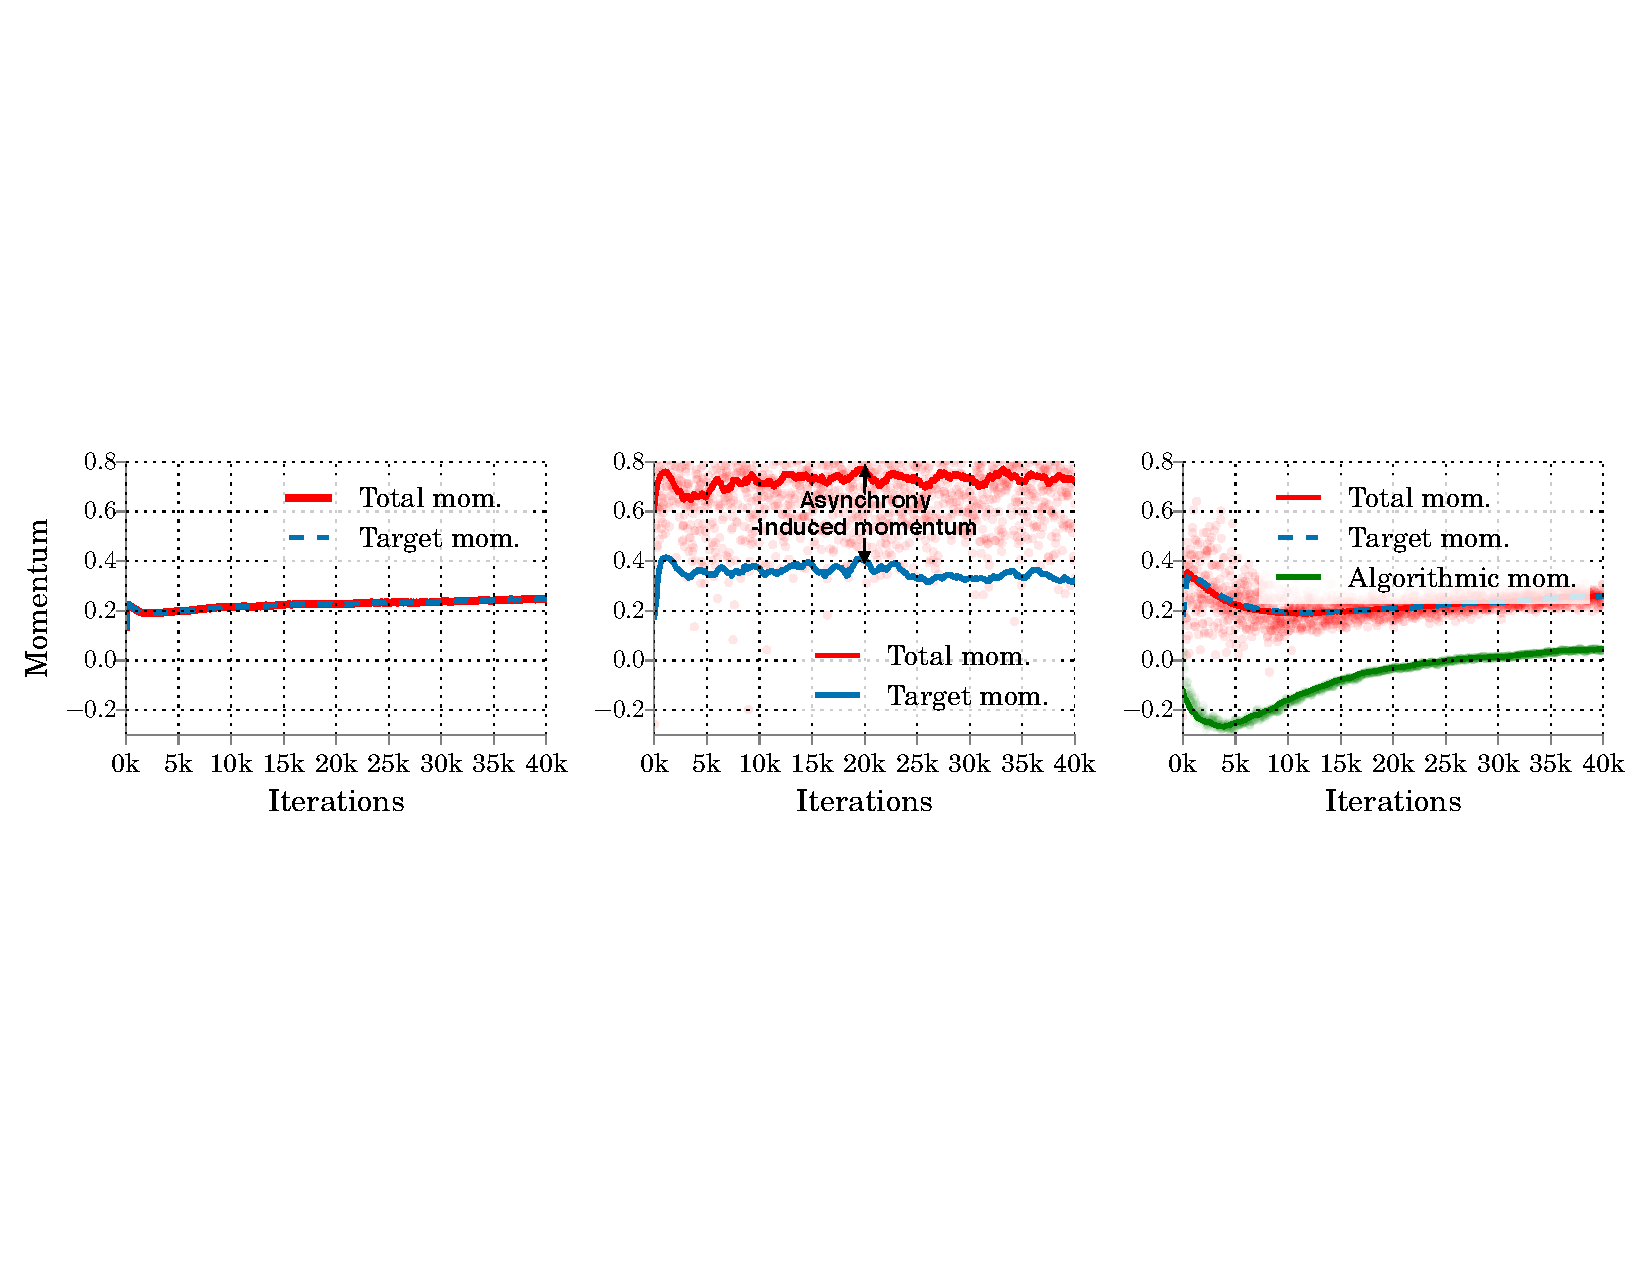
\includegraphics[width=0.95\linewidth]{experiment_results/resnet/mom_dynamic_3.pdf}
	\caption{
	Momentum dynamics on CIFAR100 ResNet.
	Running \tuner, total momentum is equal to algorithmic momentum in a synchronous setting (left). Total momentum is greater than algorithmic momentum on 16 asynchronous workers, due to asynchrony-induced momentum (middle).
	Using the momentum feedback mechanism of \asynctuner, lowers algorithmic momentum and brings total momentum to match the target value on 16 asynchronous workers (right).
	Red dots are individual total momentum estimates, $\hat{\mu}_T$, at each iteration. 
The solid red line is a running average of those estimates.	
	}
	\label{fig:we-can-measure}
\end{figure}

\paragraph{Closing the asynchrony loop}
Given a reliable measurement of $\mu_{T}$, 
we can use it to adjust the value of algorithmic momentum so that the total momentum matches the \emph{target momentum} as decided by \tuner in Algorithm~\ref{alg:basic-algo}.
\Asynctuner in Algorithm~\ref{alg:async-algo} %(in Appendix~\ref{sec:async_yf}) 
uses a simple negative feedback loop to achieve the adjustment.
Figure~\ref{fig:we-can-measure} demonstrates that under asynchrony the measured total momentum is strictly higher than the algorithmic momentum (middle plot), as expected from theory;
closing the feedback loop (right plot) leads to total momentum matching the target momentum.
Closing the loop, as we will see, improves performance significantly.
Note for asynchronous-parallel training, as the estimates and parameter tuning is unstable in the beginning when there are only a small number of iterations, we use initial learning $\frac{1}{\tau + 1}$ instead of $1.0$ to prevent overflow in the beginning. 
\begin{algorithm}[H]
	\caption{\Asynctuner}
	\begin{algorithmic}[1]
	\State Input: $\mu\gets0$, $\alpha \gets \frac{1}{\tau + 1}$, $\gamma\gets0.01, \tau$ (staleness)
	\For { $t\gets1$ to $T$}
	\State $x_t\!\gets\!x_{t - 1} + \mu (x_{t - 1} - x_{t - 2} ) - \alpha \nabla_{S_t} f(x_{t - \tau - 1} )$
	\State $\mu^*,\alpha \gets \Call{\tuner}{\nabla_{S_t} f(x_{t - \tau - 1} ), \beta}$ %(get momentum from the dynamic range)
	\State $\hat{\mu_T} 
					\gets \mathop{\mathsf{median}}\left(
							\frac{x_{t - \tau} - x_{t - \tau-1} + \alpha \nabla_{S_{t-\tau-1}} f(x_{t - \tau - 1} )}
							{x_{t - \tau-1} - x_{t - \tau-2}}
					\right)$ \Comment{Measuring total momentum}
	\State $\mu \leftarrow \mu + \gamma \cdot (\mu^* - \hat{\mu_T})$ \Comment{Closing the loop}
	\EndFor
\end{algorithmic}
\label{alg:async-algo}
\end{algorithm}




\vspace{-0.25em}
\section{Experiments}
\label{sec:experiments}
\vspace{-0.25em}
We empirically validate the importance of momentum tuning and evaluate \tuner in both synchronous (single-node) and asynchronous settings.
In synchronous settings, we first demonstrate that, with hand-tuning, momentum SGD is competitive with Adam, a state-of-the-art adaptive method.
Then, we evaluate \tuner \emph{without any hand tuning} in comparison to hand-tuned Adam and momentum SGD.
In asynchronous settings, we show that \asynctuner accelerates with momentum closed-loop control, significantly outperforming Adam.
%\emph{To eliminate influences of a specific random seed, in our synchronous and asynchronous experiments, the training loss and validation metrics are averaged from 3 runs using different random seeds.}

We evaluate on convolutional neural networks (CNN) and recurrent neural networks (RNN). For CNN, we train ResNet~\citep{he2016deep} for image recognition on CIFAR10 and CIFAR100~\citep{krizhevsky2014cifar}.
%, with regular and bottleneck building units respectively.
%We conduct experiments on both convolutional neural networks and recurrent neural networks. For convolutional neural networks, we evaluate on image recognition using a 110-layer ResNet~\citep{he2016deep} on CIFAR10~\citep{krizhevsky2014cifar} and a 164-layer ResNet on CIFAR100.
%For diversity of the models, we use regular and bottleneck building units respectively for CIFAR10 and CIFAR100.
For RNN, we train LSTMs for character-level language modeling with 
the TinyShakespeare (TS) dataset~\citep{karpathy2015visualizing}, word-level language modeling with the Penn TreeBank (PTB) ~\citep{marcus1993building}, and constituency parsing on the Wall Street Journal (WSJ) dataset~\citep{charniakparsing}.
We refer to Table~\ref{tab:model_specification} in Appendix~\ref{sec:model_spec} for model specifications. 
\emph{To eliminate influences of a specific random seed, in our synchronous and asynchronous experiments, the training loss and validation metrics are averaged from 3 runs using different random seeds.}
Across all the eight models and all experiments, we use sliding window width 20 for estimating the extreme curvature $h_max$ and $h_min$ in Algorithm~\ref{alg:curv_func}. It is selected based on the performance on PTB LSTM and CIFAR10 ResNet model. The selected sliding window width is directly applied to the other 6 models, including the convolutional sequence to sequence model in Section~\ref{sec:stability}, as well as the ResNext and Tied LSTM model in Appendix~\ref{sec:boost_exp}.

%We conduct experiments on both convolutional neural networks (CNN) and recurrent neural networks (RNN). For CNN, we evaluate on ResNet~\citep{he2016deep} for image recognition on CIFAR10~\citep{krizhevsky2014cifar} and CIFAR100, with regular and bottleneck building units respectively.
%%We conduct experiments on both convolutional neural networks and recurrent neural networks. For convolutional neural networks, we evaluate on image recognition using a 110-layer ResNet~\citep{he2016deep} on CIFAR10~\citep{krizhevsky2014cifar} and a 164-layer ResNet on CIFAR100.
%%For diversity of the models, we use regular and bottleneck building units respectively for CIFAR10 and CIFAR100.
%For RNN, we evaluate with LSTMs in 3 tasks: character-level language modeling with 
%the TinyShakespeare (TS) dataset~\citep{karpathy2015visualizing}, word-level language modeling with the Penn TreeBank (PTB) ~\citep{marcus1993building}, and constituency parsing on the Wall Street Journal (WSJ) dataset~\citep{charniakparsing}.
%We refer to Table~\ref{tab:model_specification} in Appendix~\ref{sec:model_spec} for model architecture details. 

%\vspace{-0.25em}
\subsection{Synchronous experiments}
\label{subsec:sync_exp}
\begin{figure*}[t]
\vspace{-0.75em}
\centering
	\begin{tabular}{c}
		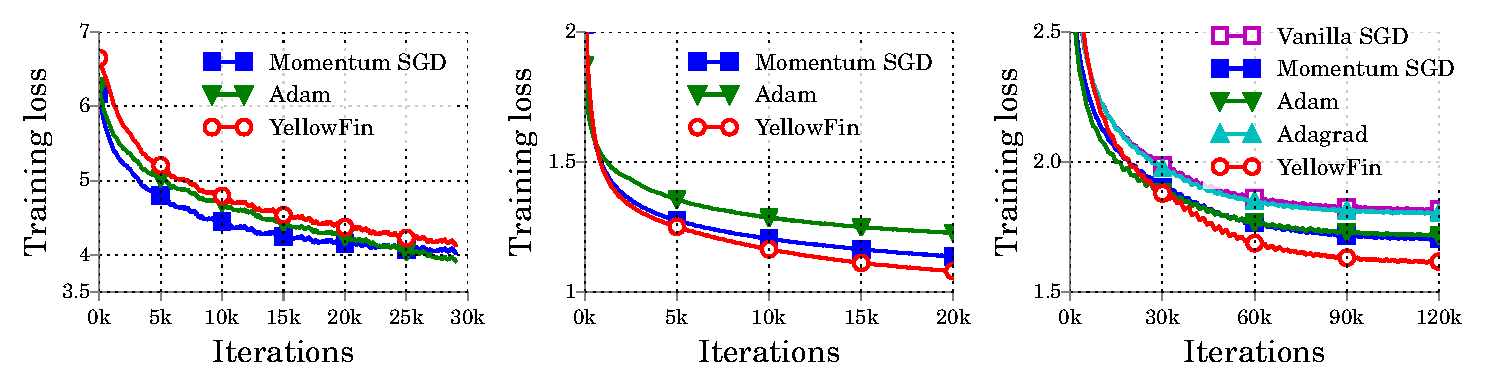
\includegraphics[width=0.925\linewidth]{experiment_results/lstm_loss_all.pdf} \\[-0.5em]
		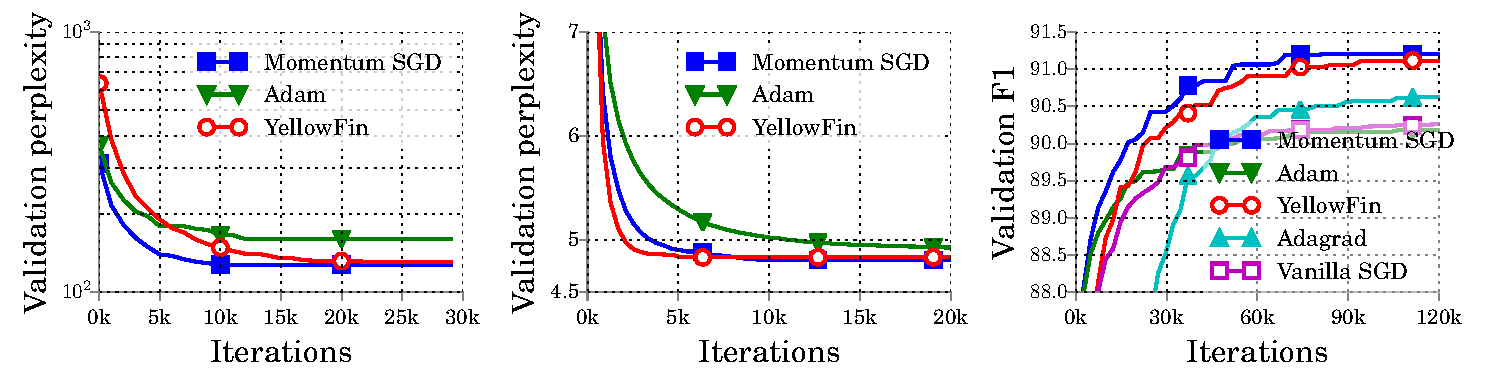
\includegraphics[width=0.925\linewidth]{experiment_results/lstm_test_all.pdf} \\[-0.5em]
	\end{tabular}
%	\vspace{-0.5em}
	\caption{
	Training loss and validation metrics on (left to right) word-level language modeling with PTB, char-level language modeling with TS and constituency parsing on WSJ. The valid. metrics are monotonic as we report the best values up to each number of iterations.}
%	\caption{
%	Training loss and validation metrics on word-level language modeling with PTB (left), char-level language modeling with TS (middle) and constituency parsing on WSJ (right). Note the validation metrics are monotonic as we report the best values up to each specific number of iterations.}
%	\vspace{-0.75em}
	\label{fig:loss_result_ptb}
%	\vspace{-0.25em}
\end{figure*}


%\begin{wrapfigure}[8]{r}{0.42\textwidth}
%\begin{minipage}{1.0\linewidth}
%\vspace{-0.3in}
%%\begin{table}[H]
%%\centering
%%\caption{
%%	Speedup of \tuner and tuned momentum SGD over tuned Adam.
%%	% The speedup is with respect to the number of iterations.
%%	%We compare our Algorithm~\ref{alg:basic-algo}) to the best configuration in tuning grid for Adam and momentum SGD. For tuned Adam and tuned momentum SGD, we take the lowest value of the smoothed training loss curve	 and report the speedup of our  to achieve the same loss. The speedup is demonstrated with respect to the number of iteraions. We run Resnet for 40k iterations, bottleneck resnet for 70k iterations and PTB LSTM for 30k Iterations.
%%	}
%%	\begin{tabular}[t]{c@{\hskip 0.6em}|c@{\hskip 0.6em}c@{\hskip 0.6em}c}
%%		\toprule
%%		 & Adam & mom.SGD & YF \\
%%		\midrule
%%		\midrule
%%		CIFAR10 & 1x & 1.71x & 1.93x  \\
%%		CIFAR100 & 1x & 1.83x & 1.35x \\
%%		PTB & 1x & 0.88x & 0.77x \\
%%		TS & 1x & 5.66x & 6.83x \\
%%		WSJ & 1x & 1.33x & 2.33x \\
%%		\bottomrule
%%	\end{tabular}
%%	\label{tab:iters_to_loss}
%%\end{table}
%% grid search version on Adam
%\begin{table}[H]
%\centering
%\caption{
%	Speedup of \tuner and tuned momentum SGD over tuned Adam.
%	% The speedup is with respect to the number of iterations.
%	%We compare our Algorithm~\ref{alg:basic-algo}) to the best configuration in tuning grid for Adam and momentum SGD. For tuned Adam and tuned momentum SGD, we take the lowest value of the smoothed training loss curve	 and report the speedup of our  to achieve the same loss. The speedup is demonstrated with respect to the number of iteraions. We run Resnet for 40k iterations, bottleneck resnet for 70k iterations and PTB LSTM for 30k Iterations.
%	}
%	\begin{tabular}[t]{c@{\hskip 0.6em}|c@{\hskip 0.6em}c@{\hskip 0.6em}c}
%		\toprule
%		 & Adam & mom.SGD & YF \\
%		\midrule
%		\midrule
%		CIFAR10 & 1x & 1.71x & 1.93x \\
%		CIFAR100 & 1x & 1.87x & 1.38x \\
%		PTB & 1x & 0.88x & 0.77x \\
%		TS & 1x & 2.49x & 3.28x \\
%		WSJ & 1x & 1.33x & 2.33x \\
%		\bottomrule
%	\end{tabular}
%	\label{tab:iters_to_loss}
%\end{table}
%\end{minipage}
%\end{wrapfigure}
We tune Adam and  momentum SGD on learning rate grids with prescribed momentum $0.9$ for SGD. We fix the parameters of Algorithm~\ref{alg:basic-algo} in all experiments, i.e.\ \tuner runs {\em without any hand tuning}.
We provide full specifications, including the learning rate (grid) and the number of iterations we train on each model in Appendix~\ref{sec:exp_spec}.
For visualization purposes, we smooth training losses with a uniform window of width $1000$. 
%\emph{We average the smoothed losses from 3 different random seeds}.
For Adam and momentum SGD on each model, we pick the configuration achieving the lowest averaged smoothed loss.
%in corresponding grids.
To compare two algorithms, we record the lowest smoothed loss achieved by both. Then the speedup is reported as the ratio of iterations to achieve this loss.
We use this setup to validate our claims.
%We tune momentum SGD and Adam on learning rate grids with prescribed momentum $0.9$ for SGD. We fix the parameters of Algorithm~\ref{alg:basic-algo} in all experiments, i.e.\ \tuner runs without any hand tuning. We provide full specifications, including the learning rate (grid) and the number of iterations we train on each model in Appendix~\ref{sec:exp_spec}.
%For visualization purposes, we smooth training losses with a uniform window of width $1000$. 
%%\emph{We average the smoothed losses from 3 different random seeds}.
%For Adam and momentum SGD on each model, we pick the configuration achieving the lowest averaged smoothed loss.
%%in corresponding grids.
%To compare two algorithms, we record the lowest smoothed loss achieved by both. Then the speedup is reported as the ratio of iterations to achieve this loss.
%We use this setup to validate our claims.
%

%%\begin{figure}[t]
%%\centering
%%	\begin{tabular}{c c}
%%		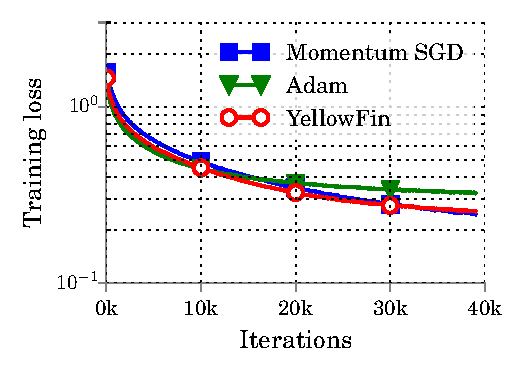
\includegraphics[width=0.45\linewidth]{experiment_results/resnet/resnet_loss.pdf} &
%%		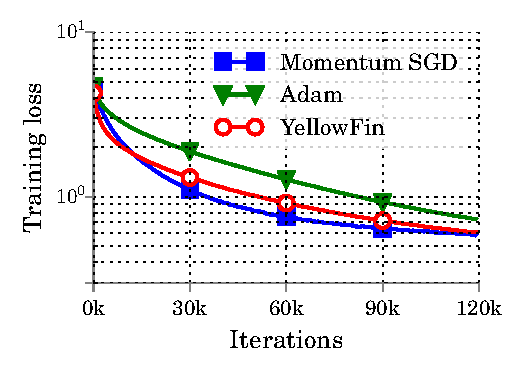
\includegraphics[width=0.45\linewidth]{experiment_results/resnet/resnet_bottleneck_loss.pdf}
%%	\end{tabular}
%%	\caption{
%%	Training loss for ResNet on CIFAR10 (left) and CIFAR100 (right, still running). }
%%	\label{fig:loss_result_cifar}
%%\end{figure}
%
%\begin{wrapfigure}[11]{r}{0.525\textwidth}
%\begin{minipage}{1.0\linewidth}
%\vspace{-0.3in}
%\begin{table}[H]
%\centering
%\caption{
%	The speedup of \tuner and tuned mom. SGD comparing to tuned Adam.
%	% The speedup is with respect to the number of iterations.
%	%We compare our Algorithm~\ref{alg:basic-algo}) to the best configuration in tuning grid for Adam and momentum SGD. For tuned Adam and tuned momentum SGD, we take the lowest value of the smoothed training loss curve	 and report the speedup of our  to achieve the same loss. The speedup is demonstrated with respect to the number of iteraions. We run Resnet for 40k iterations, bottleneck resnet for 70k iterations and PTB LSTM for 30k Iterations.
%	}
%	\begin{tabular}[t]{c@{\hskip 0.6em}|c@{\hskip 0.6em}c@{\hskip 0.6em}c}
%		\toprule
%		 & Adam & mom. SGD & \tuner \\
%		\midrule
%		\midrule
%		CIFAR10 & 1x & 1.71x & 1.93x \\
%		CIFAR100 & 1x & 1.87x & 1.38x \\
%		PTB & 1x & 0.88x & 0.77x \\
%		TS & 1x & 2.49x & 3.28x \\
%		WSJ & 1x & 1.33x & 2.33x \\
%		\bottomrule
%	\end{tabular}
%	\label{tab:iters_to_loss}
%\end{table}
%\end{minipage}
%\end{wrapfigure}
%\begin{wrapfigure}[11]{r}{0.39\textwidth}
%\begin{minipage}{1.0\linewidth}
%\vspace{-0.15in}
%%\begin{table}[H]
%%\centering
%%\caption{
%%	Speedup of \tuner and tuned momentum SGD over tuned Adam.
%%	% The speedup is with respect to the number of iterations.
%%	%We compare our Algorithm~\ref{alg:basic-algo}) to the best configuration in tuning grid for Adam and momentum SGD. For tuned Adam and tuned momentum SGD, we take the lowest value of the smoothed training loss curve	 and report the speedup of our  to achieve the same loss. The speedup is demonstrated with respect to the number of iteraions. We run Resnet for 40k iterations, bottleneck resnet for 70k iterations and PTB LSTM for 30k Iterations.
%%	}
%%	\begin{tabular}[t]{c@{\hskip 0.6em}|c@{\hskip 0.6em}c@{\hskip 0.6em}c}
%%		\toprule
%%		 & Adam & mom.SGD & YF \\
%%		\midrule
%%		\midrule
%%		CIFAR10 & 1x & 1.71x & 1.93x  \\
%%		CIFAR100 & 1x & 1.83x & 1.35x \\
%%		PTB & 1x & 0.88x & 0.77x \\
%%		TS & 1x & 5.66x & 6.83x \\
%%		WSJ & 1x & 1.33x & 2.33x \\
%%		\bottomrule
%%	\end{tabular}
%%	\label{tab:iters_to_loss}
%%\end{table}
%% grid search version on Adam
%\begin{table}[H]
%\centering
%\caption{
%	Speedup of \tuner and tuned mom. SGD over tuned Adam.
%	% The speedup is with respect to the number of iterations.
%	%We compare our Algorithm~\ref{alg:basic-algo}) to the best configuration in tuning grid for Adam and momentum SGD. For tuned Adam and tuned momentum SGD, we take the lowest value of the smoothed training loss curve	 and report the speedup of our  to achieve the same loss. The speedup is demonstrated with respect to the number of iteraions. We run Resnet for 40k iterations, bottleneck resnet for 70k iterations and PTB LSTM for 30k Iterations.
%	}
%	\begin{tabular}[t]{@{\hskip 0.3em}c@{\hskip 0.3em}|c@{\hskip 0.3em}c@{\hskip 0.3em}c@{\hskip 0.3em}}
%		\toprule
%		 & Adam & mom.SGD & YF \\
%		\midrule
%		\midrule
%		CIFAR10 & $1\times$ & $1.71\times$ & $1.93\times$ \\
%		CIFAR100 & $1\times$ & $1.87\times$ & $1.38\times$ \\
%		PTB & $1\times$ & $0.88\times$ & $0.77\times$ \\
%		TS & $1\times$ & $2.49\times$ & $3.28\times$ \\
%		WSJ & $1\times$ & $1.33\times$ & $2.33\times$ \\
%		\bottomrule
%	\end{tabular}
%	\label{tab:iters_to_loss}
%\end{table}
%\end{minipage}
%\end{wrapfigure}

%\begin{wrapfigure}[10]{r}{0.375\textwidth}
%\begin{minipage}{1.0\linewidth}
%\vspace{-0.35in}
%\begin{table}[H]
%\centering
%\caption{
%	Speedup of \tuner and tuned momentum SGD over tuned Adam.
%	% The speedup is with respect to the number of iterations.
%	%We compare our Algorithm~\ref{alg:basic-algo}) to the best configuration in tuning grid for Adam and momentum SGD. For tuned Adam and tuned momentum SGD, we take the lowest value of the smoothed training loss curve	 and report the speedup of our  to achieve the same loss. The speedup is demonstrated with respect to the number of iteraions. We run Resnet for 40k iterations, bottleneck resnet for 70k iterations and PTB LSTM for 30k Iterations.
%	}
%	\begin{tabular}[t]{c@{\hskip 0.6em}|c@{\hskip 0.6em}c@{\hskip 0.6em}c}
%		\toprule
%		 & Adam & mom.SGD & YF \\
%		\midrule
%		\midrule
%		CIFAR10 & 1x & 1.71x & 1.93x  \\
%		CIFAR100 & 1x & 1.83x & 1.35x \\
%		PTB & 1x & 0.88x & 0.77x \\
%		TS & 1x & 5.66x & 6.83x \\
%		WSJ & 1x & 1.33x & 2.33x \\
%		\bottomrule
%	\end{tabular}
%	\label{tab:iters_to_loss}
%\end{table}
% grid search version on Adam
%%%%%%%%%%%%%%% old version table %%%%%%%%%%%%%%%%%%%
%\begin{table}[H]
%\centering
%\caption{
%	Speedup of \tuner and tuned mom. SGD over tuned Adam.
%	% The speedup is with respect to the number of iterations.
%	%We compare our Algorithm~\ref{alg:basic-algo}) to the best configuration in tuning grid for Adam and momentum SGD. For tuned Adam and tuned momentum SGD, we take the lowest value of the smoothed training loss curve	 and report the speedup of our  to achieve the same loss. The speedup is demonstrated with respect to the number of iteraions. We run Resnet for 40k iterations, bottleneck resnet for 70k iterations and PTB LSTM for 30k Iterations.
%	}
%%	\vspace{-0.075in}
%%	\begin{tabular}[t]{@{\hskip 0.15em}c@{\hskip 0.15em}|c@{\hskip 0.3em}c@{\hskip 0.3em}c@{\hskip 0.15em}}
%	\begin{tabular}{c | c c c}
%		 & Adam & mom.SGD & YF \\
%		\midrule
%		\midrule
%%		CIFAR10 & $1\times$ & $1.71\times$ & $1.93\times$ \\
%%		CIFAR100 & $1\times$ & $1.87\times$ & $1.38\times$ \\
%%		PTB & $1\times$ & $0.88\times$ & $0.77\times$ \\
%%		TS & $1\times$ & $2.49\times$ & $3.28\times$ \\
%%		WSJ & $1\times$ & $1.33\times$ & $2.33\times$ \\
%		CIFAR10 & 1x & 1.71x & 1.93x \\
%		CIFAR100 & 1x & 1.87x & 1.38x \\
%		PTB & 1x & 0.88x & 0.77x \\
%		TS & 1x & 2.49x & 3.28x \\
%		WSJ & 1x & 1.33x & 2.33x \\
%		\bottomrule
%	\end{tabular}
%	\label{tab:iters_to_loss}
%\end{table}
%%%%%%%%%%%%%%%%%%%%%%%%%%%%%%%%%%%%%%%%%%%%%%%%%%%%%
%%%%%%%%%%%%%%% new version table %%%%%%%%%%%%%%%%%%%
\vspace{-0.25em}
\begin{table}[h]
\centering
\small
%	\begin{tabular}[t]{@{\hskip 0.3em}c@{\hskip 0.5em}|c@{\hskip 0.45em}c@{\hskip 0.45em}c@{\hskip 0.75em}c@{\hskip 0.75em}c@{\hskip 0.15em}}
	\begin{tabular}[t]{@{\hskip 0.5em}c@{\hskip 0.5em}|c@{\hskip 1em}c@{\hskip 1em}c@{\hskip 1em}c@{\hskip 1em}c@{\hskip 0.5em}}
%	\begin{tabular}{c | c c c c c}
		\toprule
		 & CIFAR10 & CIFAR100 & PTB & TS & WSJ \\
		\midrule
		\midrule
		Adam & 1x & 1x & 1x & 1x & 1x \\
		mom. SGD & 1.71x & 1.87x & 0.88x & 2.49x & 1.33x \\
		YF & 1.93x & 1.38x & 0.77x & 3.28x & 2.33x \\
%		CIFAR10 & 1x & 1.71x & 1.93x \\
%		CIFAR100 & 1x & 1.87x & 1.38x \\
%		PTB & 1x & 0.88x & 0.77x \\
%		TS & 1x & 2.49x & 3.28x \\
%		WSJ & 1x & 1.33x & 2.33x \\
		\bottomrule
	\end{tabular}
	\caption{
	The speedup of \tuner and tuned momentum SGD over tuned Adam on ResNet and LSTM models.
	% The speedup is with respect to the number of iterations.
	%We compare our Algorithm~\ref{alg:basic-algo}) to the best configuration in tuning grid for Adam and momentum SGD. For tuned Adam and tuned momentum SGD, we take the lowest value of the smoothed training loss curve	 and report the speedup of our  to achieve the same loss. The speedup is demonstrated with respect to the number of iteraions. We run Resnet for 40k iterations, bottleneck resnet for 70k iterations and PTB LSTM for 30k Iterations.
	}
	\label{tab:iters_to_loss}
%	\vspace{-0.85em}
\end{table}
\vspace{-0.5em}

%%%%%%%%%%%%%%%%%%%%%%%%%%%%%%%%%%%%%%%%%%%%%%%%%%%%%
%\end{minipage}
%\end{wrapfigure}
\paragraph{Momentum SGD is competitive with adaptive methods}
In Table~\ref{tab:iters_to_loss}, we compare tuned momentum SGD and tuned Adam on ResNets with training losses shown in Figure~\ref{fig:loss_result_cifar} in Appendix~\ref{sec:add_exp}. We can observe that momentum SGD
achieves $1.71$x and $1.87$x speedup to tuned Adam on CIFAR10 and CIFAR100 respectively. In Figure~\ref{fig:loss_result_ptb} and Table~\ref{tab:iters_to_loss}, 
with the exception of PTB LSTM, momentum SGD also produces better training loss, as well as better validation perplexity in language modeling and validation F1 in parsing.
For the parsing task, we also compare with tuned Vanilla SGD and AdaGrad, which are used in the NLP community.
Figure~\ref{fig:loss_result_ptb} (right) shows that \emph{fixed momentum 0.9 can already speedup Vanilla SGD by $2.73$x, achieving observably better validation F1}. %,
%a performance matched by \tuner. 
 We refer to Appendix~\ref{sec:importance_momentum} for further discussion on the importance of momentum adaptivity in \tuner.
%These observations show that momentum is critical to acceleration, and momentum SGD can be better than the state-of-the-art adaptive method in a variety of models.% 

%\begin{figure*}[t]
%%\vspace{-2.25em}
%\centering
%	\begin{tabular}{c}
%		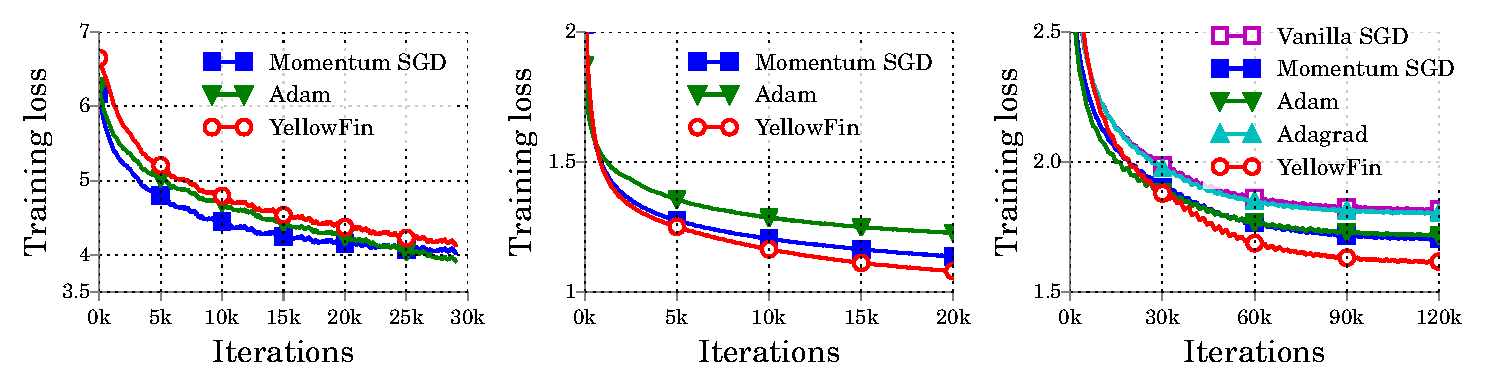
\includegraphics[width=0.925\linewidth]{experiment_results/lstm_loss_all.pdf} \\[-0.75em]
%		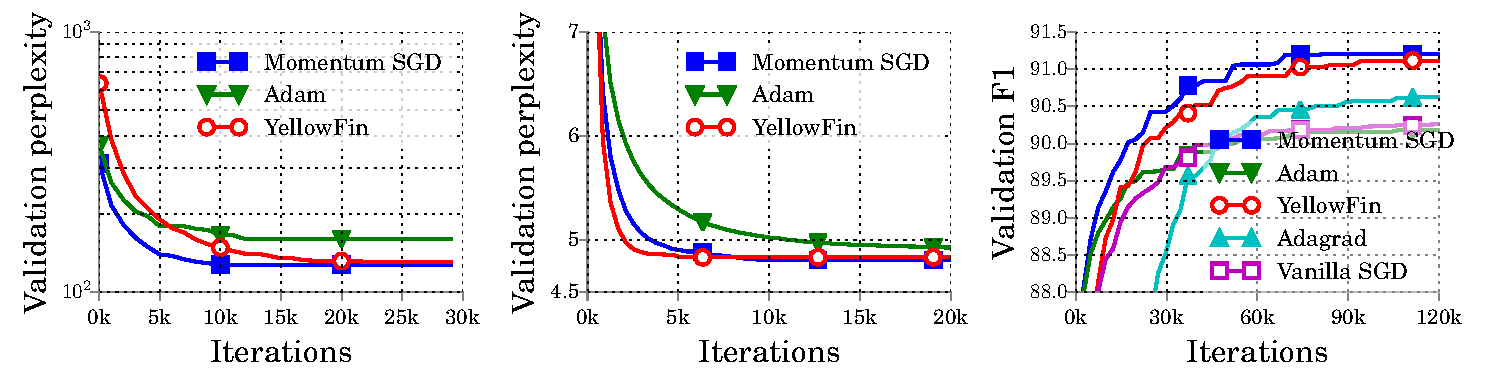
\includegraphics[width=0.925\linewidth]{experiment_results/lstm_test_all.pdf} \\[-0.5em]
%	\end{tabular}
%	\caption{
%	Training loss and test metrics on word-level language modeling with PTB (left), character-level language modeling with TS (middle) and constituency parsing on WSJ (right). Note the validation metrics are monotonic as we report the best values up to each specific number of iterations.}
%	\vspace{-0.75em}
%	\label{fig:loss_result_ptb}
%\end{figure*}


%\begin{wrapfigure}[10]{r}{0.375\textwidth}
%\begin{minipage}{1.0\linewidth}
%\vspace{-0.35in}
%%\begin{table}[H]
%%\centering
%%\caption{
%%	Speedup of \tuner and tuned momentum SGD over tuned Adam.
%%	% The speedup is with respect to the number of iterations.
%%	%We compare our Algorithm~\ref{alg:basic-algo}) to the best configuration in tuning grid for Adam and momentum SGD. For tuned Adam and tuned momentum SGD, we take the lowest value of the smoothed training loss curve	 and report the speedup of our  to achieve the same loss. The speedup is demonstrated with respect to the number of iteraions. We run Resnet for 40k iterations, bottleneck resnet for 70k iterations and PTB LSTM for 30k Iterations.
%%	}
%%	\begin{tabular}[t]{c@{\hskip 0.6em}|c@{\hskip 0.6em}c@{\hskip 0.6em}c}
%%		\toprule
%%		 & Adam & mom.SGD & YF \\
%%		\midrule
%%		\midrule
%%		CIFAR10 & 1x & 1.71x & 1.93x  \\
%%		CIFAR100 & 1x & 1.83x & 1.35x \\
%%		PTB & 1x & 0.88x & 0.77x \\
%%		TS & 1x & 5.66x & 6.83x \\
%%		WSJ & 1x & 1.33x & 2.33x \\
%%		\bottomrule
%%	\end{tabular}
%%	\label{tab:iters_to_loss}
%%\end{table}
%% grid search version on Adam
%\begin{table}[H]
%\centering
%\caption{
%	Speedup of \tuner and tuned mom. SGD over tuned Adam.
%	% The speedup is with respect to the number of iterations.
%	%We compare our Algorithm~\ref{alg:basic-algo}) to the best configuration in tuning grid for Adam and momentum SGD. For tuned Adam and tuned momentum SGD, we take the lowest value of the smoothed training loss curve	 and report the speedup of our  to achieve the same loss. The speedup is demonstrated with respect to the number of iteraions. We run Resnet for 40k iterations, bottleneck resnet for 70k iterations and PTB LSTM for 30k Iterations.
%	}
%	\vspace{-0.075in}
%	\begin{tabular}[t]{@{\hskip 0.15em}c@{\hskip 0.15em}|c@{\hskip 0.3em}c@{\hskip 0.3em}c@{\hskip 0.15em}}
%		\toprule
%		 & Adam & mom.SGD & YF \\
%		\midrule
%		\midrule
%%		CIFAR10 & $1\times$ & $1.71\times$ & $1.93\times$ \\
%%		CIFAR100 & $1\times$ & $1.87\times$ & $1.38\times$ \\
%%		PTB & $1\times$ & $0.88\times$ & $0.77\times$ \\
%%		TS & $1\times$ & $2.49\times$ & $3.28\times$ \\
%%		WSJ & $1\times$ & $1.33\times$ & $2.33\times$ \\
%		CIFAR10 & 1x & 1.71x & 1.93x \\
%		CIFAR100 & 1x & 1.87x & 1.38x \\
%		PTB & 1x & 0.88x & 0.77x \\
%		TS & 1x & 2.49x & 3.28x \\
%		WSJ & 1x & 1.33x & 2.33x \\
%		\bottomrule
%	\end{tabular}
%	\label{tab:iters_to_loss}
%\end{table}
%\end{minipage}
%\end{wrapfigure}
\paragraph{\tuner can match hand-tuned momentum SGD and can outperform hand-tuned Adam}% on ResNets and LSTMs}
In our experiments, 
\tuner, without any hand-tuning, yields training loss matching hand-tuned momentum SGD for all the ResNet and LSTM models in Figure~\ref{fig:loss_result_ptb} and~\ref{fig:loss_result_cifar}.  
When comparing to tuned Adam in Table~\ref{tab:iters_to_loss}, except being slightly slower on PTB LSTM, \tuner achieves $1.38$x to $3.28$x speedups in training losses on the other four models. \emph{More importantly, \tuner consistently shows better validation metrics than tuned Adam in Figure~\ref{fig:loss_result_ptb}}. It demonstrates that \tuner can match tuned momentum SGD and outperform tuned state-of-the-art adaptive optimizers. % in training deep neural networks.% in a large class of models.
In Appendix~\ref{sec:boost_exp}, we show \tuner further speeding up with finer-grain manual learning rate tuning.
%As careful optimizer tuning can further improve model performance in fixed training time, we refer to Appendix~\ref{sec:boost_exp} on auxiliary manual learning rate tuning for \tuner.

%%In our experiments, 
%%\tuner, without any hand-tuning, yields speedups from to 1.32x to 3.28x on ResNets and LSTMs in comparison to tuned momentum SGD.  
%When comparing to tuned Adam in Table~\ref{tab:iters_to_loss}, \tuner achieves speedups from 1.32x to 3.28x in training losses. \emph{More importantly, \tuner consistently shows better test metrics than tuned momentum SGD and Adam}. It demonstrates that \tuner can outperform hand-tuned state-of-the-art adaptive and non-adaptive optimizers.% in a large class of models.
\begin{figure*}
\centering	
\begin{tabular}{c c c}
	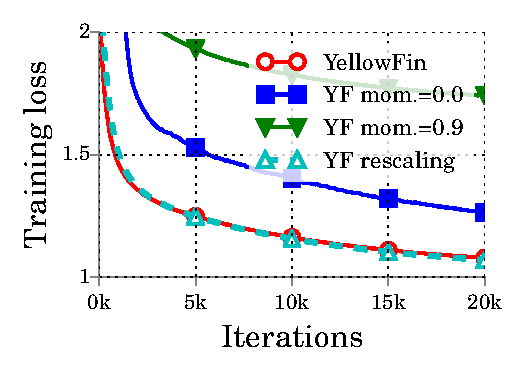
\includegraphics[width=0.31\linewidth]{experiment_results/tf_charrnn_train_loss_fix_mom_and_lr_rescaling_cmp.pdf} &
	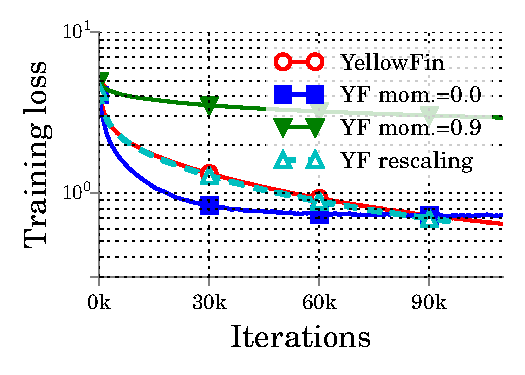
\includegraphics[width=0.31\linewidth]{experiment_results/resnet/resnet_bottleneck_loss_fix_mom_and_lr_rescaling_cmp} &
	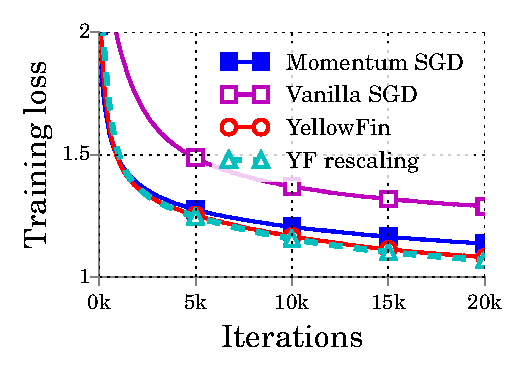
\includegraphics[width=0.31\linewidth]{experiment_results/tf_charrnn_train_loss_mom_vanilla_yf.pdf}
\end{tabular}
\caption{The importance of adaptive momentum: Training loss comparison between \tuner with adaptive momentum and \tuner with fixed momentum value; this comparison is conducted on TS LSTM (left) and CIFAR100 ResNet (right). Learning rate scaling based on \tuner tuned momentum can match the performance of full \tuner (right) on the TS LSTM. However without the \tuner tuned momentum, hand-tuned Vanilla SGD demonstrates observably larger training loss than momentum based methods, including full \tuner, \tuner learning rate rescaling and hand-tuned momentum SGD (with the same learning rate search grid as with Vanilla SGD.)}
\label{fig:cmp_fix_mom}
\end{figure*}

\paragraph{The importance of adaptive momentum in \tuner}
In Definition~\ref{def:GCN}, we noticed that the optimally tuned $\mu^*$ is highly objective-dependent. Empirically, We indeed observe a wide range of tuned momentum $\mu$ from YF; it ranges from smaller than 0.03 in the PTM LSTM to 0.89 for ResNext. To further validate the importance of momentum adaptivity in \tuner, we perform an ablation study to demonstrate the importance of objective-dependent momentum adaptivity in \tuner with CIFAR100 ResNet and TS LSTM. In the experiments, \tuner tunes the learning rate. Instead of also using the momentum tuned by YF, we continuously feed objective-agnostic prescribed momentum value $0.0$ and $0.9$ to the underlying momentum SGD optimizer which YF is tuning. In Figure~\ref{fig:cmp_fix_mom}, when comparing to \tuner with prescribed momentum 0.0 or 0.9, \tuner with adaptively tuned momentum achieves observably faster convergence on both TS LSTM and CIFAR100 ResNet. From a more practical perspective, in Figure~\ref{fig:loss_result_ptb} (bottom right) and Figure~\ref{fig:cmp_fix_mom} (right), we also observe that hand-tuned optimizer without momentum, i.e. Vanilla SGD, typically can not match the performance of momentum based methods, including \tuner and momentum SGD hand-tuned using the same learning rate grid as with Vanilla SGD. However in \tuner, we can rescale the learning rate based on the \tuner tuned momentum $\mu_t$, and use 0 momentum in the model updates to match the performance of momentum based methods. Specifically, we rescale the \tuner tuned learning rate $\alpha_t$ with $1/(1 - \mu_t)$ \footnote{Let $v_t = x_t - x_{t - 1}$ be the model update, this rescaling is motivated with the fact that $v_{t+1} = \mu_t v_{t} - \alpha_t \nabla f(x_t)$. Assuming the $v_t$ evolves smoothly, we have $v_t \approx \alpha_t/(1-\mu_t) \nabla f(x_t)$.}. Model updates with this rescaled learning rate and 0 momentum can demonstrate training loss closely matching those of \tuner and hand-tuned momentum SGD for WSJ LSTM in Figure~\ref{fig:loss_result_ptb} (bottom right) and TS LSTM in Figure~\ref{fig:cmp_fix_mom} (right).



%\begin{wrapfigure}[9]{r}{0.34\linewidth}
%\vspace{-0.6in}
%\begin{minipage}{1.0\linewidth}
%	\begin{figure}[H]
%		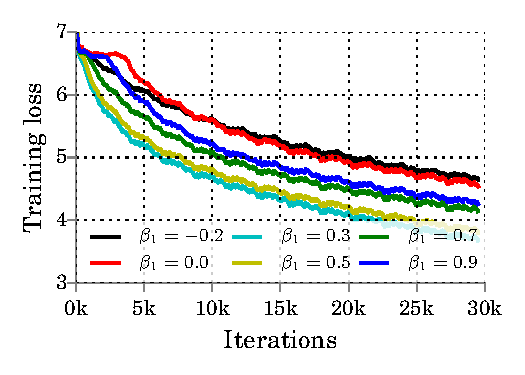
\includegraphics[width=0.975\linewidth]{experiment_results/ptb/adam_stale_15_tuning.pdf}
%			\vspace{-1.5em}
%		\caption{Hand-tuning Adam's momentum under asynchrony.}
%		\label{fig:adam_async_mom}
%	\end{figure}
%%	\vspace{-1.5em}
%%	\begin{figure}[H]
%%		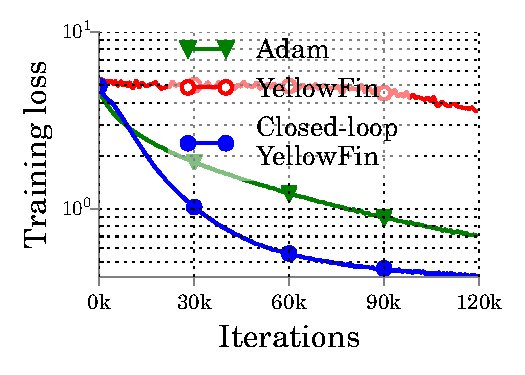
\includegraphics[width=0.975\linewidth]{experiment_results/resnet/resnet_bottleneck_cmp_tuner_adam.pdf}
%%%		\caption{Adam, \tuner and \asynctuner on CIFAR100 with 16 async. workers. Sync. baseline uses \tuner.}
%%	\vspace{-1.5em}
%%		\caption{Asynchronous performance on CIFAR100 ResNet.}
%%		\label{fig:full_async_cmp}
%%	\end{figure}
%\end{minipage}	
%\end{wrapfigure}

%\begin{wrapfigure}[9]{R}{0.5\linewidth}
%\vspace{-0.575in}
%%\vspace{-0.75in}
%\begin{minipage}{\linewidth}
%%	\begin{figure}[H]
%%		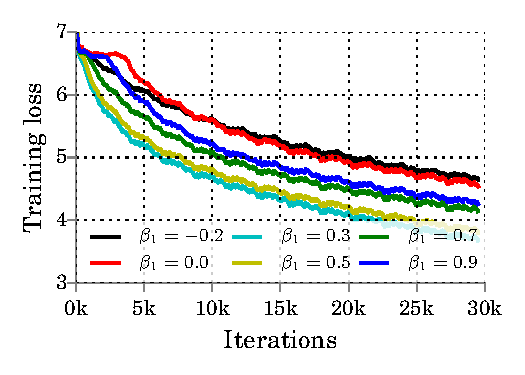
\includegraphics[width=\linewidth]{experiment_results/ptb/adam_stale_15_tuning.pdf}
%%			\vspace{-1.5em}
%%		\caption{Hand-tuning Adam's momentum under asynchrony.}
%%		\label{fig:adam_async_mom}
%%	\end{figure}
%%	\vspace{-1.5em}
%	\begin{figure}[H]
%		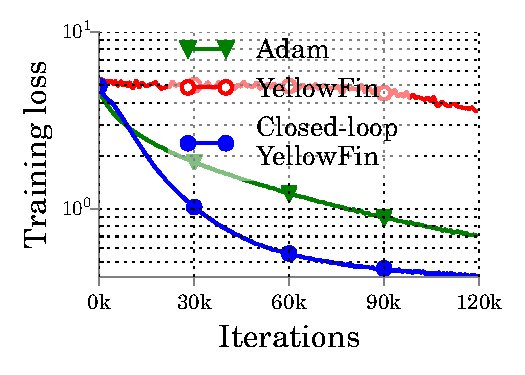
\includegraphics[width=1.05\linewidth]{experiment_results/resnet/resnet_bottleneck_cmp_tuner_adam.pdf}
%%		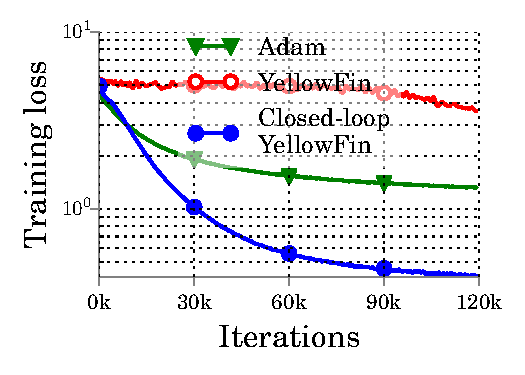
\includegraphics[width=0.975\linewidth]{experiment_results/resnet/resnet_bottleneck_cmp_tuner_adam_default_adam.pdf}
%%		\caption{Adam, \tuner and \asynctuner on CIFAR100 with 16 async. workers. Sync. baseline uses \tuner.}
%	\vspace{-1.75em}
%		\caption{Asynchronous performance on CIFAR100 ResNet.}
%		\label{fig:full_async_cmp}
%	\end{figure}
%\end{minipage}	
%\end{wrapfigure}
%%\vspace*{5.0em}
\subsection{Asynchronous experiments}
\label{sec:async_exp}
%\vspace{-1em}
In this section, we evaluate \asynctuner with focus on the number of iterations to reach a certain solution. 
To that end, we run $16$ asynchronous workers on a single machine and force them to update the model in a round-robin fashion,
i.e. the gradient is delayed for $15$ iterations.
%We demonstrate
%%(1) Adam suffers a convergence speed penalty due to not tuning momentum in asynchronous settings;
%(1) \asynctuner (cf.\ Section~\ref{sec:async_tuner}) improves the convergence of \tuner dramatically, which leads to
%(3) \asynctuner having much faster convergence than Adam. 
%     
%\paragraph{State-of-the-art adaptive methods suffer from lack of momentum tuning} We conduct experiments on PTB LSTM with 16 asynchronous workers using Adam.
%Fixing the learning rate to the value achieving the lowest smoothed loss in Section~\ref{subsec:sync_exp}, we sweep the smoothing parameter $\beta_1$~\citep{kingma2014adam} of the first order moment estimate in grid $\{-0.2, 0.0, 0.3, 0.5, 0.7, 0.9\}$. $\beta_1$ serves the same role as momentum in SGD and we call it the momentum in Adam. Figure~\ref{fig:adam_async_mom} shows tuning momentum for Adam under asynchrony gives measurably better training loss. 
%This result emphasizes the importance of momentum tuning in asynchronous settings and suggests that state-of-the-art adaptive methods pay a penalty for using prescribed momentum.
%
%\begin{wrapfigure}[10]{r}{0.34\linewidth}
%\vspace{-0.35in}
%\begin{minipage}{1.0\linewidth}
%%	\begin{figure}[H]
%%		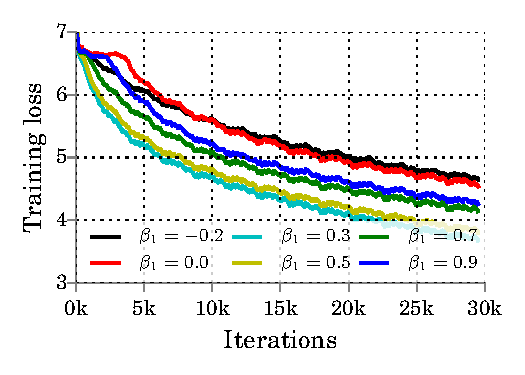
\includegraphics[width=\linewidth]{experiment_results/ptb/adam_stale_15_tuning.pdf}
%%			\vspace{-1.5em}
%%		\caption{Hand-tuning Adam's momentum under asynchrony.}
%%		\label{fig:adam_async_mom}
%%	\end{figure}
%%	\vspace{-1.5em}
%	\begin{figure}[H]
%		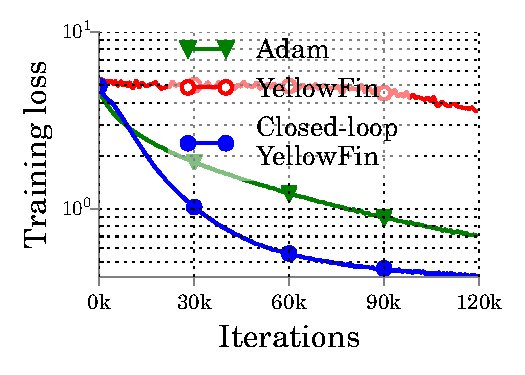
\includegraphics[width=0.975\linewidth]{experiment_results/resnet/resnet_bottleneck_cmp_tuner_adam.pdf}
%%		\caption{Adam, \tuner and \asynctuner on CIFAR100 with 16 async. workers. Sync. baseline uses \tuner.}
%	\vspace{-1.5em}
%		\caption{Asynchronous performance on CIFAR100 ResNet.}
%		\label{fig:full_async_cmp}
%	\end{figure}
%\end{minipage}	
%\end{wrapfigure}
%\paragraph{Closing the loop improves convergence under staleness}
%We compare the performance of \tuner in Algorithm~\ref{alg:basic-algo} and \asynctuner in Algorithm~\ref{alg:async-algo} on the 164-layer bottleneck ResNet. We conduct experiments using 16 asynchronous workers.
%In Figure~\ref{fig:adam_under_staleness} (right), 
%Figure~\ref{fig:full_async_cmp} 
Figure~\ref{fig:spotlight} (right) 
presents training losses on the CIFAR100 ResNet, using \tuner in Algorithm~\ref{alg:basic-algo}, \asynctuner in Algorithm~\ref{alg:async-algo} and Adam with the learning rate achieving the best smoothed loss in Section~\ref{subsec:sync_exp}.
We can observe closed-loop \tuner achieves $20.1$x speedup to \tuner, 
%Consequently, closed-loop \tuner achieves 5.09x speedup over Adam.
and consequently a $2.69$x speedup to Adam.
This demonstrates that (1) \asynctuner accelerates by reducing algorithmic momentum to compensate for asynchrony and (2) can converge in less iterations than Adam in asynchronous-parallel training. 
%We notice that \asynctuner achieves very similar loss as the synchronous baseline near the end.
%It suggests an almost $16$x wall-clock time speedup by parallelizing asynchronously.
%\vspace{-0.5em}
%\paragraph{Closed-loop \tuner outperforms Adam in asynchrony} 
%We run Adam with 16 workers on CIFAR100 ResNet using the learning rate achieving the lowest smoothed loss in Section~\ref{subsec:sync_exp}.
%Shown in Figure~\ref{fig:full_async_cmp}, Adam slows down dramatically due to asynchrony, while closed-loop \tuner, with feedback gain $\gamma=0.01$, demonstrates up to 2.69x speedup  over Adam.
%It shows \asynctuner can significantly outperform the state-of-the-art in asynchronous settings.

%\begin{figure}[t]
%\centering
%	\begin{tabular}{c c}
%		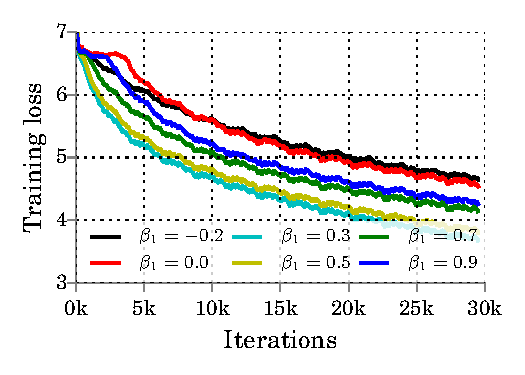
\includegraphics[width=0.45\linewidth]{experiment_results/ptb/adam_stale_15_tuning.pdf} &
%		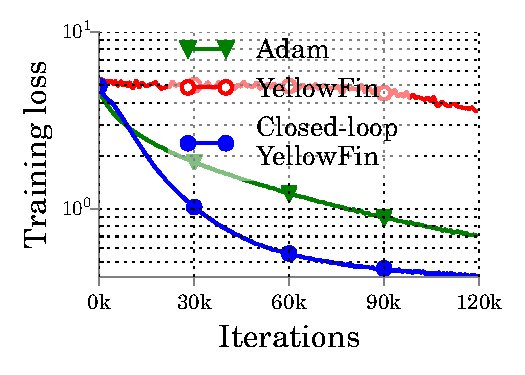
\includegraphics[width=0.45\linewidth]{experiment_results/resnet/resnet_bottleneck_cmp_tuner_adam.pdf}
%	\end{tabular}
%	\caption{
%	Hand-tuning Adam's momentum under asynchrony (left) on PTB LSTM. Asynchronous performance comparison (right) on CIFAR100 ResNet.}
%	\label{fig:adam_under_staleness}
%\end{figure}



%% async experiment backup version
%\begin{wrapfigure}[9]{r}{0.34\linewidth}
%\vspace{-0.6in}
%\begin{minipage}{1.0\linewidth}
%	\begin{figure}[H]
%		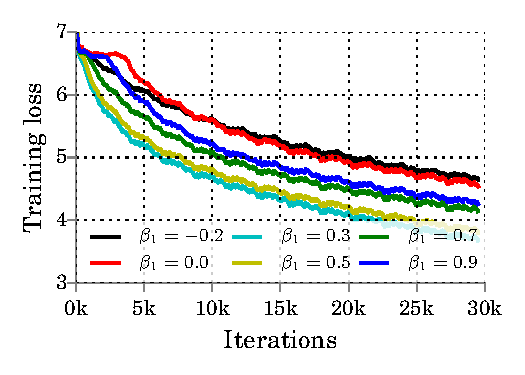
\includegraphics[width=0.975\linewidth]{experiment_results/ptb/adam_stale_15_tuning.pdf}
%			\vspace{-1.5em}
%		\caption{Hand-tuning Adam's momentum under asynchrony.}
%		\label{fig:adam_async_mom}
%	\end{figure}
%%	\vspace{-1.5em}
%%	\begin{figure}[H]
%%		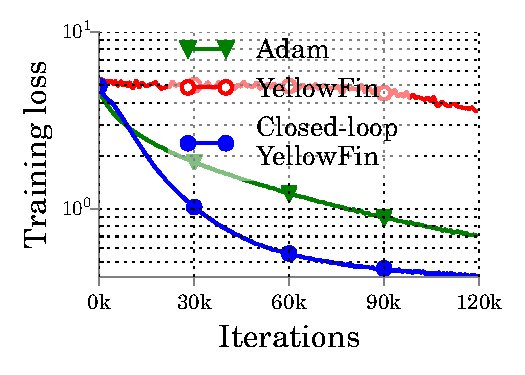
\includegraphics[width=0.975\linewidth]{experiment_results/resnet/resnet_bottleneck_cmp_tuner_adam.pdf}
%%%		\caption{Adam, \tuner and \asynctuner on CIFAR100 with 16 async. workers. Sync. baseline uses \tuner.}
%%	\vspace{-1.5em}
%%		\caption{Asynchronous performance on CIFAR100 ResNet.}
%%		\label{fig:full_async_cmp}
%%	\end{figure}
%\end{minipage}	
%\end{wrapfigure}
%\subsection{Asynchronous experiments}
%In this section, we evaulate \tuner in an asynchronous-parallel setting,
%where we focus on {\em statistical efficiency}: the number of iterations to reach a certain solution. 
%To that end, we run $M$ asynchronous workers on a single machine and force them to update the model in a round-robin fashion,
%i.e. the staled gradient is delayed for $(M-1)$ iterations.
%We demonstrate
%(1) Adam suffers a convergence speed penalty due to not tuning momentum in asynchronous settings;
%(2) \asynctuner (cf.\ Section~\ref{sec:async_tuner}) improves the convergence of \tuner dramatically, which leads to
%(3) \asynctuner having much faster convergence than Adam. 
%     
%
%\paragraph{State-of-the-art adaptive methods suffer from lack of momentum tuning} We conduct experiments on PTB LSTM with 16 asynchronous workers using Adam.
%Fixing the learning rate to the value achieving the lowest smoothed loss in Section~\ref{subsec:sync_exp}, we sweep the smoothing parameter $\beta_1$~\citep{kingma2014adam} of the first order moment estimate in grid $\{-0.2, 0.0, 0.3, 0.5, 0.7, 0.9\}$. $\beta_1$ serves the same role as momentum in SGD and we call it the momentum in Adam. Figure~\ref{fig:adam_async_mom} shows tuning momentum for Adam under asynchrony gives measurably better training loss. 
%This result emphasizes the importance of momentum tuning in asynchronous settings and suggests that state-of-the-art adaptive methods pay a penalty for using prescribed momentum.
%
%\begin{wrapfigure}[10]{r}{0.34\linewidth}
%\vspace{-0.35in}
%\begin{minipage}{1.0\linewidth}
%%	\begin{figure}[H]
%%		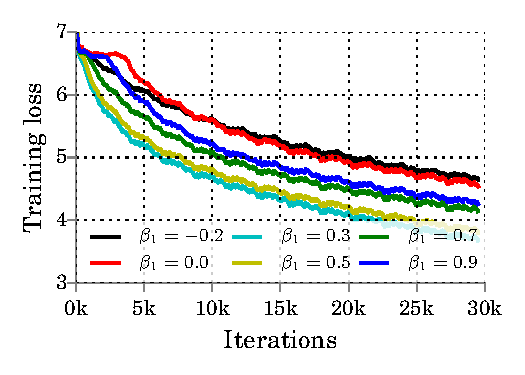
\includegraphics[width=\linewidth]{experiment_results/ptb/adam_stale_15_tuning.pdf}
%%			\vspace{-1.5em}
%%		\caption{Hand-tuning Adam's momentum under asynchrony.}
%%		\label{fig:adam_async_mom}
%%	\end{figure}
%%	\vspace{-1.5em}
%	\begin{figure}[H]
%		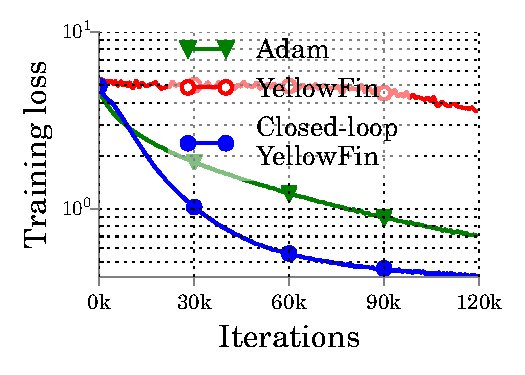
\includegraphics[width=0.975\linewidth]{experiment_results/resnet/resnet_bottleneck_cmp_tuner_adam.pdf}
%%		\caption{Adam, \tuner and \asynctuner on CIFAR100 with 16 async. workers. Sync. baseline uses \tuner.}
%	\vspace{-1.5em}
%		\caption{Asynchronous performance on CIFAR100 ResNet.}
%		\label{fig:full_async_cmp}
%	\end{figure}
%\end{minipage}	
%\end{wrapfigure}
%\paragraph{Closing the loop improves convergence under staleness}
%We compare the performance of \tuner in Algorithm~\ref{alg:basic-algo} and \asynctuner in Algorithm~\ref{alg:async-algo} on the 164-layer bottleneck ResNet. We conduct experiments using 16 asynchronous workers.
%%In Figure~\ref{fig:adam_under_staleness} (right), 
%In Figure~\ref{fig:full_async_cmp}, 
%we observe \tuner without closed-loop momentum control decrease slowly before 90k iterations. Consequently, the closed-loop \tuner achieves more than 20.1x speedup to reach the lowest loss from \tuner after 120k iterations.
%This demonstrates that \asynctuner accelerates by effectively reducing algorithmic momentum to compensate for asynchrony. 
%%We notice that \asynctuner achieves very similar loss as the synchronous baseline near the end.
%%It suggests an almost $16$x wall-clock time speedup by parallelizing asynchronously.
%\vspace{-0.5em}
%\paragraph{Closed-loop \tuner outperforms Adam in asynchrony} We run Adam with 16 workers on CIFAR100 ResNet using the learning rate achieving the lowest smoothed loss in Section~\ref{subsec:sync_exp}.
%Shown in Figure~\ref{fig:full_async_cmp}, Adam slows down dramatically due to asynchrony, while closed-loop \tuner, with feedback gain $\gamma=0.01$, demonstrates up to 2.69x speedup  over Adam.
%%It shows \asynctuner can significantly outperform the state-of-the-art in asynchronous settings.
%
%%\begin{figure}[t]
%%\centering
%%	\begin{tabular}{c c}
%%		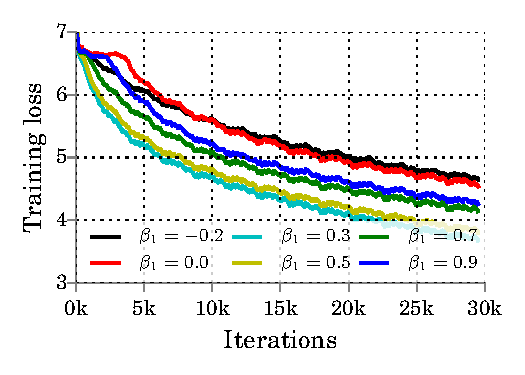
\includegraphics[width=0.45\linewidth]{experiment_results/ptb/adam_stale_15_tuning.pdf} &
%%		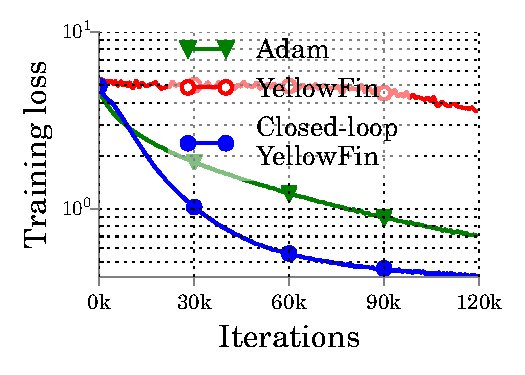
\includegraphics[width=0.45\linewidth]{experiment_results/resnet/resnet_bottleneck_cmp_tuner_adam.pdf}
%%	\end{tabular}
%%	\caption{
%%	Hand-tuning Adam's momentum under asynchrony (left) on PTB LSTM. Asynchronous performance comparison (right) on CIFAR100 ResNet.}
%%	\label{fig:adam_under_staleness}
%%\end{figure}




 







 




\vspace{-0.25em}
\section{Related work}
\label{sec:related}
\vspace{-0.3em}
Many techniques have been proposed on tuning hyperparameters for optimizers.~\citet{bergstra2012random} investigate random search for general tuning of  hyperparameters. 
Bayesian approaches~\cite{snoek2012practical} model evaluation metrics as samples from a Gaussian process guiding optimal hyperparameter search. 
Another trend is the adaptive methods which require less manual tuning than SGD:
Adagrad~\cite{duchi2011adaptive} is one of the first method with per-dimension learning rate, followed by RMSProp~\cite{tieleman2012lecture} and Adam~\cite{chilimbi2014project} using different learning rate rules. 
\citet{schaul2013no} use a noisy quadratic model similar to ours,
however they tune per-variable learning rates and 
do not use momentum.


\vspace{-0.25em}
\section{Discussion}
\label{sec:discussion}
\vspace{-0.3em}
We presented \tuner, the first optimization method that automatically tunes momentum as well as the learning rate of momentum SGD. 
\tuner outperforms the state-of-the-art in optimizing a large class of models both in synchronous and asynchronous settings.
It estimates statistics purely from the gradients of a running system,
and then tunes the hyperparameters of momentum SGD based on noisy, local quadratic approximations.
As future work, we believe that more accurate curvature estimation methods,
like the $bbprop$ method~\cite{martens2012estimating} can further improve \tuner.
We also believe that our closed-loop momentum control mechanism in Section~\ref{sec:async_tuner} 
could be applied to other adaptive methods and improve performances in asynchronous-parallel settings.


\section{Acknowledgements}
We thank Bryan He, Paroma Varma, Chris De Sa and Theodoros Rekatsinas for helpful discussions. We gratefully acknowledge the support of the Defense Advanced Research Projects Agency (DARPA) SIMPLEX program under No. N66001-15-C-4043, the D3M program under No. FA8750-17-2-0095, the National Science Foundation (NSF) CAREER Award under No. IIS- 1353606, the Office of Naval Research (ONR) under awards No. N000141210041 and No. N000141310129, a Sloan Research Fellowship, the Moore Foundation, an Okawa Research Grant, Toshiba, and Intel. Any opinions, findings, and conclusions or recommendations expressed in this material are those of the authors and do not necessarily reflect the views of DARPA, NSF, ONR, or the U.S. government.


\bibliographystyle{unsrtnat}
\bibliography{arxiv}

\appendix 
\newpage
\onecolumn
\section{Proof of Lemma~\ref{lem:robustness}}
\label{sec:proof_robustness}
To prove Lemma~\ref{lem:robustness}, we first prove a more generalized version in Lemma~\ref{lem:robustness_general}. By restricting $f$ to be a one dimensional quadratics function, the generalized curvature $h_t$ itself is the only eigenvalue. We can prove Lemma~\ref{lem:robustness} as a straight-forward corollary. Lemma~\ref{lem:robustness_general} also implies, in the multiple dimensional correspondence of~\eqref{equ:one_dim_22_rec}, the spectral radius $\rho(\mat{A}_t)=\sqrt{\mu}$ if the curvature on all eigenvector directions (eigenvalue) satisfies~\eqref{eqn:robust_region}.

\begin{lemma}
\label{lem:robustness_general}
Let the gradients of a function $f$ be described by
\begin{equation}
	\nabla f(\mat{x}_t) = \mat{H}(\mat{x}_t) (\mat{x}_t - \mat{x}^*),
\end{equation}
with $\mat{H}(\bm{x}_t) \in \mathbb{R}^n \mapsto \mathbb{R}^{n\times n}$.
Then the momentum update can be expressed as a linear operator:
\begin{align}
{\begin{pmatrix}
\mat{y}_{t+1}\\
\mat{y}_t \\
\end{pmatrix}}
=
{\begin{pmatrix}
\mat{I}-\alpha \mat{H}(\mat{x}_t) + \mu \mat{I} & - \mu \mat{I} \\
\mat{I} & \mat{0} \\
\end{pmatrix}}
{\begin{pmatrix}
\mat{y}_t \\
\mat{y}_{t-1} \\
\end{pmatrix}}
=\mat{A}_t
{\begin{pmatrix}
\mat{y}_t \\
\mat{y}_{t-1} \\
\end{pmatrix}},
\end{align}
where $\mat{y}_t\triangleq \mat{x}_t - \mat{x}^*$.
Now, assume that the following condition holds for all eigenvalues $\lambda(\mat{H}(\bm{x}_t))$ of $\mat{H}(\bm{x}_t)$:
\begin{align}
{(1-\sqrt{\mu})^2\over \alpha} &\leq \lambda(\mat{H}(\bm{x}_t)) \leq {(1+\sqrt{\mu})^2\over \alpha}.
\label{equ:control_condition}
\end{align}
then the spectral radius of $\mat{A}_t$ is controlled by momentum with
$	\rho(\mat{A}_t) = \sqrt{\mu}.$

\begin{proof}
Let $\lambda_t$ be an eigenvalue of matrix $\mat{A}_t$, it gives 
$\det\left(\mat{A}_t - \lambda_t \mat{I} \right) = 0$. 
We define the blocks in $\mat{A}_t$ as $\mat{C} = \mat{I} - \alpha \mat{H}_t + \mu \mat{I} - \lambda_t \mat{I}$, $\mat{D} = -\mu \mat{I}$,
$\mat{E} = \mat{I}$ and $\mat{F} = -\lambda_t \mat{I}$ which gives
\[
\det \left( \mat{A}_t - \lambda_t \mat{I}\right) = \det{\mat{F}} \det{\left(\mat{C} - \mat{D} \mat{F}^{-1}
\mat{E} \right)} = 0
\]
assuming generally $\mat{F}$ is invertible. Note we use $\mat{H}_t\triangleq\mat{H}(\mat{x}_t)$ for simplicity in writing. The equation $\det{\left(\mat{C} - \mat{D} \mat{F}^{-1}
\mat{E} \right)} = 0$ implies that
\begin{equation}
\det \left( \lambda_t^2\mat{I} - \lambda_t \mat{M}_t + \mu \mat{I} \right) = 0
\label{equ:control_condition_2}
\end{equation}
with $\mat{M}_t = \left( \mat{I} - \alpha \mat{H}_t + \mu \mat{I} \right)$. In other words, $\lambda_t$ satisfied that $\lambda_t^2 - \lambda_t \lambda(\mat{M}_t) + \mu = 0$ with $\lambda(\mat{M}_t)$ being one eigenvalue of $\mat{M_t}$. I.e.
\begin{equation}
	\lambda_t = \frac{\lambda(\mat{M}_t) \pm \sqrt{\lambda(\mat{M}_t)^2 - 4\mu}}{2}
\end{equation}

On the other hand,~\eqref{equ:control_condition} guarantees that $(1 - \alpha \lambda(\mat{H}_t) + \mu)^2 \leq 4\mu$. We know both $\mat{H}_t$ and $\mat{I} - \alpha \mat{H}_t + \mu \mat{I}$ are symmetric. Thus for all eigenvalues $\lambda(\mat{M}_t)$ of $\mat{M}_t$, we have $\lambda(\mat{M}_t)^2 = (1 - \alpha \lambda(\mat{H}_t) + \mu)^2 \leq 4\mu$ which guarantees $| \lambda_t | = \sqrt{\mu}$ for all $\lambda_t$. As the spectral radius is equal to the magnitude of the largest eigenvalue of $\mat{A}_t$, we have the spectral radius of $\mat{A}_t$ being $\sqrt{\mu}$.


\end{proof}
	
\end{lemma}


\section{Proof of Lemma~\ref{lem:main_lemma}}
We first prove Lemma~\ref{lem:bias_rec} and Lemma~\ref{lem:var_rec} as preparation for the proof of Lemma~\ref{lem:main_lemma}. After the proof for one dimensional case, we discuss the trivial generalization to multiple dimensional case.
\begin{lemma}
\label{lem:bias_rec}
	Let the $h$ be the curvature of a one dimensional quadratic function $f$ and $\overline{x}_t = \E x_t$. We assume, without loss of generality, the optimum point of $f$ is $x^{\star}=0$. Then we have the following recurrence
	\begin{equation} 
		\begin{pmatrix}
			\overline{x}_{t + 1} \\
			\overline{x}_t
		\end{pmatrix} = 
		\begin{pmatrix}
			1-\alpha h + \mu & - \mu\\
			1 & 0 \\
		\end{pmatrix}^{t}
		\begin{pmatrix}
			x_1 \\
			x_0
		\end{pmatrix}
		\label{equ:bias_rec}
	\end{equation} 
	\begin{proof}
		From the recurrence of momentum SGD, % in~\eqref{equ:momentum_sgd}, 
		we have
		\begin{equation*}
			\begin{aligned}
				\E x_{t + 1} = & \E [ x_{t} - \alpha \nabla f_{S_t} (x_t) + \mu (x_t - x_{t - 1} ) ]\\
							= & \E_{x_{t}}	[ x_{t} - \alpha \E_{S_t} \nabla f_{S_t} (x_t) + \mu (x_t - x_{t - 1} ) ] \\
							= & \E_{x_{t}}	[ x_{t} - \alpha h x_t + \mu (x_t - x_{t - 1} ) ] \\
							= & (1 - \alpha h + \mu)\overline{x}_t - \mu\overline{x}_{t - 1}
			\end{aligned}
		\end{equation*}
		By putting the equation in to matrix form,~\eqref{equ:bias_rec} is a straight-forward result from unrolling the recurrence for $t$ times. Note as we set $x_1 = x_0$ with no uncertainty in momentum SGD, we have $[\overline{x}_0, \overline{x}_1] = [x_0, x_1]$.
	\end{proof}
\end{lemma}

\begin{lemma}
\label{lem:var_rec}
	Let $U_t=\E ( x_t - \overline{x}_t ) ^2$ and $V_t= \E (x_t - \overline{x}_t)(x_{t-1} - \overline{x}_{t-1})$ with $\overline{x}_t$ being the expectation of $x_t$. For quadratic function $f(x)$ with curvature $h \in \mathbb{R}$, We have the following recurrence
		\begin{equation} 
		\begin{pmatrix}
			U_{t+1} \\
			U_t \\
			V_{t + 1}
		\end{pmatrix} = 
		(\mat{I} - \mat{B}^{\top})(\mat{I} - \mat{B})^{-1}
		\begin{pmatrix}
			\alpha^2 C \\
			0 \\
			0
		\end{pmatrix}
	\end{equation}
	where 
	\begin{equation}
		\mat{B} = 
		\begin{pmatrix}
		(1-\alpha h + \mu)^2 &  \mu^2 & -2\mu(1-\alpha h + \mu)\\
		1 & 0 & 0 \\
		1-\alpha h + \mu & 0 & - \mu
		\end{pmatrix}
	\end{equation}
	and $C = \E ( \nabla f_{S_t}(x_t) - \nabla f(x_t) )^2$ is the variance of gradient on minibatch $S_t$.
	
	\begin{proof}
		We prove by first deriving the recurrence for $U_t$ and $V_t$ respectively and combining them in to a matrix form. For $U_t$, we have
		\begin{equation}
		\begin{aligned}
			U_{t + 1} = & \E ( x_{t+1} - \overline{x}_{t + 1} )^2\\
			 = & \E ( x_{t} - \alpha \nabla f_{S_t}(x_t) + \mu (x_{t} - x_{t - 1} ) - (1 - \alpha h + \mu) \overline{x}_t + \mu \overline{x}_{t - 1} )^2 \\
			 = & \E ( x_{t} - \alpha \nabla f(x_t) + \mu (x_{t} - x_{t - 1} ) - (1 - \alpha h + \mu) \overline{x}_t + \mu \overline{x}_{t - 1}  + \alpha (\nabla f(x_t) - \nabla f_{S_t}(x_t)) )^2 \\
			 = & \E ( (1 - \alpha h + \mu) (x_t - \overline{x}_t)  - \mu(x_{t - 1} - \overline{x}_{t - 1} ) )^2 + \alpha^2 \E ( \nabla f(x_t) - \nabla f_{S_t}(x_t) )^2 \\
			 = & (1 - \alpha h + \mu)^2 \E ( x_t - \overline{x}_t )^2 -2 \mu (1 - \alpha h + \mu) \E (x_t - \overline{x}_t)(x_{t - 1} - \overline{x}_{t - 1} ) \\
			 & + \mu^2\E ( x_{t-1} - \overline{x}_{t-1} )^2+ \alpha^2 C
		\end{aligned}
		\label{equ:U_term}
		\end{equation}
		where the cross terms cancels due to the fact $\E_{S_t} [\nabla f(x_t) - \nabla f_{S_t}(x_t)]=0$ in the third equality. 
		
		For $V_t$, we can similarly derive
		\begin{equation}
		\begin{aligned}			
			V_t = & \E (x_t - \overline{x}_t) (x_{t-1} - \overline{x}_{t-1} ) \\
			= & \E ( (1 - \alpha h + \mu) (x_{t-1} - \overline{x}_{t-1} ) - \mu (x_{t-2} - \overline{x}_{t-2}) + \alpha (\nabla f(x_t) - \nabla f_{S_t}(x_t) ) ) (x_{t-1} - \overline{x}_{t-1} ) \\
			= & (1 - \alpha h + \mu)\E ( x_{t-1} - \overline{x}_{t-1} )^2 - \mu \E (x_{t-1} - \overline{x}_{t-1})(x_{t-2} - \overline{x}_{t-2})
		\end{aligned}
		\label{equ:V_term}
		\end{equation}
		Again, the term involving $\nabla f(x_t) - \nabla f_{S_t}(x_t)$ cancels in the third equality as a results of $\E_{S_t} [\nabla f(x_t) - \nabla f_{S_t}(x_t)]=0$.~\eqref{equ:U_term} and~\eqref{equ:V_term} can be jointly expressed in the following matrix form
		\begin{equation}
		\begin{aligned}
			\begin{pmatrix}
			U_{t+1} \\
			U_t \\
			V_{t + 1}
		\end{pmatrix}= \mat{B} 
		\begin{pmatrix}
			U_t \\
			U_{t-1} \\
			V_t
		\end{pmatrix} + 
		\begin{pmatrix}
			\alpha^2 C \\
			0 \\
			0
		\end{pmatrix}
		=\sum\limits_{i = 0}^{t-1} \mat{B}^{i} \begin{pmatrix}
			\alpha^2 C \\
			0 \\
			0
		\end{pmatrix} + \mat{B}^t \begin{pmatrix}
			U_1 \\
			U_0 \\
			V_1
		\end{pmatrix}
		= (\mat{I} - \mat{B}^t)(\mat{I} - \mat{B})^{-1}
		\begin{pmatrix}
			\alpha^2 C \\
			0 \\
			0
		\end{pmatrix}.
		\end{aligned}
		\end{equation}
		Note the second term in the second equality is zero because $x_0$ and $x_1$ are deterministic. Thus $U_1\!=\!U_0\!=\!V_1\!=\!0$.
	\end{proof}
\end{lemma}

According to Lemma~\ref{lem:bias_rec} and~\ref{lem:var_rec}, we have $\E ( \overline{x}_t - x^{*} )^2 = (\mat{e}^{\top}_1 \mat{A}^t [x_1, x_0]^{\top})^2$ and $\E ( x_t - \overline{x}_t )^2=\alpha^2 C \mat{e}^{\top}_1 (\mat{I} - \mat{B}^t)(\mat{I} - \mat{B})^{-1}\mat{e}_1$ where $\mat{e}_1 \in \mathbb{R}^n$ has all zero entries but the first dimension. Combining these two terms, we prove Lemma~\ref{lem:main_lemma}. Though the proof here is for one dimensional quadratics, it trivially generalizes to multiple dimensional quadratics. Specifically, we can decompose the quadratics along the eigenvector directions, and then apply Lemma~\ref{lem:main_lemma} to each eigenvector direction using the corresponding curvature $h$ (eigenvalue). By summing quantities in~\eqref{equ:squared_dist_exact} for all eigenvector directions, we can achieve the multiple dimensional correspondence of~\eqref{equ:squared_dist_exact}.




\section{Proof of Lemma~\ref{lem:spectral_var_control}}
Again we first present a proof of a multiple dimensional generalized version of Lemma~\ref{lem:spectral_var_control}. The proof of Lemma~\ref{lem:spectral_var_control} is a one dimensional special case of Lemma~\ref{lem:spectral_var_control_multi}. Lemma~\ref{lem:spectral_var_control_multi} also implies that for multiple dimension quadratics, the corresponding spectral radius $\rho(\mat{B})=\mu$ if ${(1-\sqrt{\mu})^2\over \alpha} \leq h \leq {(1+\sqrt{\mu})^2\over \alpha}$ on all the eigenvector directions with $h$ being the eigenvalue (curvature).
\begin{lemma}
\label{lem:spectral_var_control_multi}
Let $\mat{H}\in\mathbb{R}^{n\times n}$ be a symmetric matrix and $\rho(\mat{B})$ be the spectral radius of matrix 
\begin{equation}
	%\rho_V(\alpha, \mu) = \rho \left(
\mat{B} = {\begin{pmatrix}
(\mat{I}-\alpha \mat{H} + \mu \mat{I})^{\top}(\mat{I}-\alpha \mat{H} + \mu \mat{I}) &  \mu^2 \mat{I} & -2\mu(\mat{I}-\alpha \mat{H} + \mu \mat{I})\\
\mat{I} & \mat{0} & \mat{0} \\
\mat{I}-\alpha \mat{H} + \mu \mat{I} & \mat{0} & - \mu \mat{I} 
\end{pmatrix}}
	%\right)
\end{equation}
We have $\rho(\mat{B})=\mu$ if all eigenvalues $\lambda(\mat{H})$ of $\mat{H}$ satisfies
\begin{equation}
{(1-\sqrt{\mu})^2\over \alpha} \leq \lambda(\mat{H}) \leq {(1+\sqrt{\mu})^2\over \alpha}.
\label{equ:control_condition_var}
\end{equation}

\begin{proof}
	Let $\lambda$ be an eigenvalue of matrix $\mat{B}$, it gives 
$\det\left(\mat{B} - \lambda \mat{I} \right) = 0$ which can be alternatively expressed as
\begin{equation}	
\det \left( \mat{B} - \lambda \mat{I}\right) = \det{\mat{F}} \det{\left(\mat{C} - \mat{D} \mat{F}^{-1}
\mat{E} \right)} = 0
\label{equ:control_condition_var_1}
\end{equation}
assuming $\mat{F}$ is invertible, i.e. $\lambda + \mu \neq 0$, where the blocks in $\mat{B}$ 
\begin{equation*}
		\mat{C} = \left( { \begin{array}{c c}
 			\mat{M}^{\top}\mat{M} - \lambda \mat{I} &  \mu^2 \mat{I} \\
 			\mat{I} & - \lambda \mat{I}
 		\end{array} } \right), 
 		\mat{D} = \left( { \begin{array}{c}
 			-2\mu \mat{M} \\
 			\mat{0}
 		\end{array}}\right),
 		\mat{E} = \left( {\begin{array}{c}
 			\mat{M} \\
 			\mat{0}
 		\end{array}} \right)^{\top},
 		\mat{F} = -\mu \mat{I} - \lambda \mat{I}
	\end{equation*}
	with $\mat{M}=\mat{I}-\alpha \mat{H} + \mu \mat{I}$.~\eqref{equ:control_condition_var_1} can be transformed using straight-forward algebra as
	\begin{equation}
		\det \left( \begin{array}{c c}
 			(\lambda - \mu) \mat{M}^{\top}\mat{M} - (\lambda + \mu) \lambda \mat{I} & (\lambda + \mu)\mu^2 \mat{I} \\
 			(\lambda + \mu) \mat{I} & -(\lambda + \mu)\lambda \mat{I}
 		\end{array} \right) = 0
		\label{equ:control_condition_var_2}	
	\end{equation}
	Using similar simplification technique as in~\eqref{equ:control_condition_var_1}, we can further simplify into
	\begin{equation}
		(\lambda - \mu)\det \left( (\lambda + \mu)^2 \mat{I} - \lambda \mat{M}^{\top}\mat{M} \right) = 0
	\end{equation}
	if $\lambda \neq \mu$, as $(\lambda + \mu)^2 \mat{I} - \lambda \mat{M}^{\top}\mat{M}$ is diagonalizable, we have $(\lambda + \mu)^2 - \lambda \lambda(\mat{M})^2 = 0$ with $\lambda(\mat{M})$ being an eigenvalue of symmetric $\mat{M}$. The analytic solution to the equation can be explicitly expressed as
	\begin{equation}
		\lambda = \frac{\lambda(\mat{M})^2 - 2\mu \pm \sqrt{(\lambda(\mat{M})^2 - 2\mu)^2 - 4\mu^2}}{2}.
		\label{equ:control_condition_var_3}	
	\end{equation}
	
	When the condition in~\eqref{equ:control_condition_var} holds, we have $\lambda(M)^2=(1 - \alpha \lambda(\mat{H}) + \mu)^2 \leq 4\mu$. One can verify that 
	
	\begin{equation}
		\begin{aligned}
			(\lambda(\mat{M})^2 - 2\mu)^2 - 4\mu^2 & = && (\lambda(\mat{M})^2 - 4\mu)\lambda(\mat{M})^2 \\
			& = &&\left( (1 - \alpha \rho(\mat{H} ) + \mu)^2 - 4\mu\right)\lambda(\mat{M})^2 \\
			& \leq && 0
		\end{aligned}
	\end{equation}
	Thus the roots in~\eqref{equ:control_condition_var_3} are conjugate with $| \lambda | = \mu$. In conclusion, the condition in~\eqref{equ:control_condition_var} can guarantee all the eigenvalues of $\mat{B}$ has magnitude $\mu$. Thus the spectral radius of $\mat{B}$ is controlled by $\mu$.
\end{proof}

\end{lemma}



%\input{multi_dim}
%\input{dist_small_lstm}
\section{Analytical solution to~\eqref{equ:noisy_min}}
\label{sec:opt}
The problem in~\eqref{equ:noisy_min} does not need iterative solver but has an analytical solution. Substituting only the second constraint, the objective becomes $p(x)=x^2D^2 + (1-x)^4/h_{\min}^2C$ with $x=\sqrt{\mu} \in [0, 1)$. By setting the gradient of $p(x)$ to 0, we can get a cubic equation whose root $x=\sqrt{\mu_p}$ can be computed in closed form using Vieta's substitution. As $p(x)$ is uni-modal in $[0, 1)$, the optimizer for \eqref{equ:noisy_min} is exactly the maximum of $\mu_p$ and $(\sqrt{h_{\max}/h_{\min} }-1 )^2 / (\sqrt{h_{\max}/h_{\min}}+1)^2$, the right hand-side of the first constraint in~\eqref{equ:noisy_min}.

%\begin{figure*}
%\vspace{-1em}
\centering
%\includegraphics[width=0.99\linewidth, trim={10cm 0 0 0},clip]{../yellowfin_iclr2018/manuscript_for_revision/experiment_results/resnet/mom_dynamic_3_annotated.pdf}
\includegraphics[width=0.99\linewidth]{../yellowfin_iclr2018/manuscript_for_revision/experiment_results/resnet/mom_dynamic_3_annotated.pdf}
	\vspace{-0.5em}
	\caption{
	When running \tuner, total momentum $\hat{\mu}_t$ equals algorithmic value in synchronous settings (left); $\hat{\mu}_t$ is greater than algorithmic value on 16 asynchronous workers (middle).
	\Asynctuner automatically lowers algorithmic momentum and brings total momentum to match the target value (right).
%Red dots are measured $\hat{\mu}_t$ at every step with red line as its running average.
	Red dots are total momentum estimates, $\hat{\mu}_T$, at each iteration. 
The solid red line is a running average of $\hat{\mu}_T$.
%	When running \tuner, total momentum $\hat{\mu}_t$ is greater than algorithmic value on 16 asynchronous workers (left).
%	\Asynctuner automatically lowers algorithmic momentum and matches total momentum to the target value (right).
%%Red dots are measured $\hat{\mu}_t$ at every step with red line as its running average.
%	Red dots are total momentum estimates, $\hat{\mu}_T$, at each iteration. 
%    The solid red line is a running average of $\hat{\mu}_T$.	
	}
	\label{fig:we-can-measure}
%\vspace{-0.35em}
\end{figure*}

\section{\Asynctuner}
\label{sec:async_tuner}

Asynchrony is a parallelization technique that avoids synchronization barriers \citep{recht2011hogwild}. 
In this section, we propose a {\em closed momentum loop} variant of \tuner to accelerate convergence in asynchronous training. 
%To handle the momentum dynamics of asynchronous parallelism, we propose a {\em closed momentum loop} variant of \tuner.
After some preliminaries, we show the mechanism of the extension: 
it measures the dynamics on a running system and controls momentum with a negative feedback loop.
\paragraph{Preliminaries}
%Asynchrony is a popular parallelization technique \citep{recht2011hogwild} that avoids synchronization barriers.
When training on $M$ asynchronous workers, staleness (the number of model updates between a worker's read and write operations) is on average $\tau=M-1$,
i.e., the gradient in the SGD update is delayed by $\tau$ iterations as $\nabla f_{S_{t - \tau}}(x_{t - \tau} )$.
Asynchrony yields faster steps, but can
increase the number of iterations to achieve the same solution,
a tradeoff between hardware and statistical 
efficiency~\citep{DBLP:journals/pvldb/ZhangR14}.
\citet{mitliagkas2016asynchrony} interpret asynchrony as added momentum dynamics.
Experiments in \citet{hadjis2016omnivore} support this finding, and demonstrate that reducing algorithmic momentum can compensate for asynchrony-induced momentum
and significantly reduce the number of iterations for convergence.
Motivated by that result, we use the model
in~\eqref{equ:exp_async_update_app}, where the total momentum, $\mu_T$, includes both asynchrony-induced and algorithmic  momentum, $\mu$, in~\eqref{eqn:momentum_gd}.
\begin{equation}
	\mathbb{E}[ x_{t+1} - x_t ] 
	= \mu_T \mathbb{E}[x_t - x_{t-1}] - \alpha \mathbb{E}\nabla f(x_{t})
\label{equ:exp_async_update_app}
\end{equation}
We will use this expression to design an estimator for the value of total momentum, $\hat{\mu}_T$.
This estimator is a basic building block of \asynctuner, that {\em removes the need to manually compensate for the effects of asynchrony}.



\paragraph{Measuring the momentum dynamics}
\Asynctuner estimates total momentum $\mu_{T}$ on a running system and uses a negative feedback loop to adjust algorithmic momentum accordingly.
Equation~\eqref{equ:exp_async_update} gives an estimate of $\hat{\mu}_T$ on a system with staleness $\tau$, based on \eqref{equ:exp_async_update}.
\begin{align}
\hat{\mu}_T
					= \mathop{\mathsf{median}}\left(
							\frac{x_{t - \tau} - x_{t - \tau-1} + \alpha \nabla_{S_{t-\tau -1}} f(x_{t - \tau - 1} )}
							{x_{t - \tau-1} - x_{t - \tau-2}}
					\right)
\label{eqn:momentum_measurement}
\end{align}
We use $\tau$-stale model values to match the staleness of the gradient,  and perform all operations in an elementwise fashion. 
This way we get a total momentum measurement from each variable; 
the median combines them into a more robust estimate.

\paragraph{Closing the asynchrony loop}
Given a reliable measurement of $\mu_{T}$, 
we can use it to adjust the value of algorithmic momentum so that the total momentum matches the \emph{target momentum} as decided by \tuner in Algorithm~\ref{alg:basic-algo}.
\Asynctuner in Algorithm~\ref{alg:async-algo} %(in Appendix~\ref{sec:async_yf}) 
uses a simple negative feedback loop to achieve the adjustment.
%Figure~\ref{fig:we-can-measure} demonstrates that under asynchrony the measured total momentum is strictly higher than the algorithmic momentum (middle plot), as expected from theory;
%closing the feedback loop (right plot) leads to total momentum matching the target momentum.
%Closing the loop, as we will see, improves performance significantly.
%Note for asynchronous-parallel training, as the estimates and parameter tuning is unstable in the beginning when there are only a small number of iterations, we use initial learning $\frac{1}{\tau + 1}$ instead of $1.0$ to prevent overflow in the beginning. 

%\begin{algorithm}[H]
%	\caption{\Asynctuner}
%	\begin{algorithmic}[1]
%%	\State Input: $\mu\gets0$, $\alpha \gets \frac{1}{\tau + 1}$, $\gamma\gets0.01, \tau$ (staleness)
%	\State Input: $\mu\gets0$, $\alpha \gets 0.0001$, $\gamma\gets0.01, \tau$ (staleness)
%	\For { $t\gets1$ to $T$}
%	\State $x_t\!\gets\!x_{t - 1} + \mu (x_{t - 1} - x_{t - 2} ) - \alpha \nabla_{S_t} f(x_{t - \tau - 1} )$
%	\State $\mu^*,\alpha \gets \Call{\tuner}{\nabla_{S_t} f(x_{t - \tau - 1} ), \beta}$ %(get momentum from the dynamic range)
%	\State $\hat{\mu_T} 
%					\gets \mathop{\mathsf{median}}\left(
%							\frac{x_{t - \tau} - x_{t - \tau-1} + \alpha \nabla_{S_{t-\tau-1}} f(x_{t - \tau - 1} )}
%							{x_{t - \tau-1} - x_{t - \tau-2}}
%					\right)$ \Comment{Measuring total momentum}
%	\State $\mu \leftarrow \mu + \gamma \cdot (\mu^* - \hat{\mu_T})$ \Comment{Closing the loop}
%	\EndFor
%\end{algorithmic}
%\label{alg:async-algo}
%\end{algorithm}




%In Section~\ref{sec:async_tuner}, we briefly discuss the mechanism of our designed \Asynctuner in asynchronous-parallel setting. In this appendix, we expand the details in total momentum estimator, $\hat{\mu_T}$, and present the full \Asynctuner in Algorithm~\ref{alg:async-algo} with extensive discussion.
%\paragraph{Measuring the momentum dynamics}
%Remember, we use the formula in~\eqref{equ:exp_async_update_app} to model the momentum dynamics in asynchronous-parallel systems
%\Asynctuner estimates total momentum $\mu_{T}$ on a running system and uses a negative feedback loop to adjust algorithmic momentum accordingly.
%\begin{equation}
%	\mathbb{E}[ x_{t+1} - x_t ] 
%	= \mu_T \mathbb{E}[x_t - x_{t-1}] - \alpha \mathbb{E}\nabla f(x_{t})
%\label{equ:exp_async_update_app}
%\end{equation}
%Equation~\eqref{eqn:momentum_measurement_app} gives an estimate of $\hat{\mu_T}$ on a system with staleness $\tau$, based on \eqref{equ:exp_async_update_app}.
%\begin{align}
%\hat{\mu_T}
%					= \mathop{\mathsf{median}}\left(
%							\frac{x_{t - \tau} - x_{t - \tau-1} + \alpha \nabla_{S_{t-\tau -1}} f(x_{t - \tau - 1} )}
%							{x_{t - \tau-1} - x_{t - \tau-2}}
%					\right)
%\label{eqn:momentum_measurement_app}
%\end{align}
%We use $\tau$-stale model values to match the staleness of the gradient,  and perform all operations in an elementwise fashion. 
%This way we get a total momentum measurement from each variable; 
%the median combines them into a more robust estimate.
%
%%\label{subsec:closed_loop_YF}
%%\begin{figure}
%%\centering
%%\includegraphics[width=0.95\linewidth]{experiment_results/resnet/mom_dynamic_3_annotated.pdf}
%%	\caption{
%%	Momentum dynamics on CIFAR100 ResNet.
%%	Running \tuner, total momentum is equal to algorithmic momentum in a synchronous setting (left). Total momentum is greater than algorithmic momentum on 16 asynchronous workers, due to asynchrony-induced momentum (middle).
%%	Using the momentum feedback mechanism of \asynctuner, lowers algorithmic momentum and brings total momentum to match the target value on 16 asynchronous workers (right).
%%	Red dots are individual total momentum estimates, $\hat{\mu}_T$, at each iteration. 
%%The solid red line is a running average of those estimates.	
%%	}
%%	\label{fig:we-can-measure}
%%\end{figure}
%
%\paragraph{Closing the asynchrony loop}
%Given a reliable measurement of $\mu_{T}$, 
%we can use it to adjust the value of algorithmic momentum so that the total momentum matches the \emph{target momentum} as decided by \tuner in Algorithm~\ref{alg:basic-algo}.
%\Asynctuner in Algorithm~\ref{alg:async-algo} %(in Appendix~\ref{sec:async_yf}) 
%uses a simple negative feedback loop to achieve the adjustment.
%%Figure~\ref{fig:we-can-measure} demonstrates that under asynchrony the measured total momentum is strictly higher than the algorithmic momentum (middle plot), as expected from theory;
%%closing the feedback loop (right plot) leads to total momentum matching the target momentum.
%%Closing the loop, as we will see, improves performance significantly.
%%%Note for asynchronous-parallel training, as the estimates and parameter tuning is unstable in the beginning when there are only a small number of iterations, we use initial learning $\frac{1}{\tau + 1}$ instead of $1.0$ to prevent overflow in the beginning. 
%%
%%%\begin{algorithm}[H]
%%%	\caption{\Asynctuner}
%%%	\begin{algorithmic}[1]
%%%%	\State Input: $\mu\gets0$, $\alpha \gets \frac{1}{\tau + 1}$, $\gamma\gets0.01, \tau$ (staleness)
%%%	\State Input: $\mu\gets0$, $\alpha \gets 0.0001$, $\gamma\gets0.01, \tau$ (staleness)
%%%	\For { $t\gets1$ to $T$}
%%%	\State $x_t\!\gets\!x_{t - 1} + \mu (x_{t - 1} - x_{t - 2} ) - \alpha \nabla_{S_t} f(x_{t - \tau - 1} )$
%%%	\State $\mu^*,\alpha \gets \Call{\tuner}{\nabla_{S_t} f(x_{t - \tau - 1} ), \beta}$ %(get momentum from the dynamic range)
%%%	\State $\hat{\mu_T} 
%%%					\gets \mathop{\mathsf{median}}\left(
%%%							\frac{x_{t - \tau} - x_{t - \tau-1} + \alpha \nabla_{S_{t-\tau-1}} f(x_{t - \tau - 1} )}
%%%							{x_{t - \tau-1} - x_{t - \tau-2}}
%%%					\right)$ \Comment{Measuring total momentum}
%%%	\State $\mu \leftarrow \mu + \gamma \cdot (\mu^* - \hat{\mu_T})$ \Comment{Closing the loop}
%%%	\EndFor
%%%\end{algorithmic}
%%%\label{alg:async-algo}
%%%\end{algorithm}
%%
%
%
%




\begin{algorithm}[h]
	\caption{\Asynctuner}
	\begin{algorithmic}[1]
%	\State Input: $\mu\gets0$, $\alpha \gets \frac{1}{\tau + 1}$, $\gamma\gets0.01, \tau$ (staleness)
	\State Input: $\mu\gets0$, $\alpha \gets 0.0001$, $\gamma\gets0.01, \tau$ (staleness)
	\For { $t\gets1$ to $T$}
	\State $x_t\!\gets\!x_{t - 1} + \mu (x_{t - 1} - x_{t - 2} ) - \alpha \nabla_{S_t} f(x_{t - \tau - 1} )$
	\State $\mu^*,\alpha \gets \Call{\tuner}{\nabla_{S_t} f(x_{t - \tau - 1} ), \beta}$ %(get momentum from the dynamic range)
	\State $\hat{\mu_T} 
					\gets \mathop{\mathsf{median}}\left(
							\frac{x_{t - \tau} - x_{t - \tau-1} + \alpha \nabla_{S_{t-\tau-1}} f(x_{t - \tau - 1} )}
							{x_{t - \tau-1} - x_{t - \tau-2}}
					\right)$ \Comment{Measuring total momentum}
	\State $\mu \leftarrow \mu + \gamma \cdot (\mu^* - \hat{\mu_T})$ \Comment{Closing the loop}
	\EndFor
\end{algorithmic}
\label{alg:async-algo}
\end{algorithm}


%%%%%%%%%%%%%%%%% latest backup version %%%%%%%%%%%%%%%%%%%%%%%%%%%%%%%%%%%%
%Asynchrony is a parallelization technique that avoids synchronization barriers \citep{recht2011hogwild}. 
%%In this section, we propose a {\em closed momentum loop} variant of \tuner to accelerate convergence in asynchronous training. 
%%To handle the momentum dynamics of asynchronous parallelism, we propose a {\em closed momentum loop} variant of \tuner.
%%After some preliminaries, we show the mechanism of the extension: 
%%it measures the dynamics on a running system and controls momentum with a negative feedback loop.
%%\paragraph{Preliminaries}
%%Asynchrony is a popular parallelization technique \citep{recht2011hogwild} that avoids synchronization barriers.
%%When training on $M$ asynchronous workers, staleness (the number of model updates between a worker's read and write operations) is on average $\tau=M-1$,
%%i.e., the gradient in the SGD update is delayed by $\tau$ iterations as $\nabla f_{S_{t - \tau}}(x_{t - \tau} )$.
%%It yields faster steps, but can
%%increase the number of iterations needed,
%%a tradeoff between hardware and statistical 
%%efficiency~\citep{DBLP:journals/pvldb/ZhangR14}.
%It yields better hardware efficiency, i.e. faster steps, but can
%increase the number of iterations to a given metric, i.e. statistical efficiency, as a tradeoff~\citep{DBLP:journals/pvldb/ZhangR14}.
%%a tradeoff between hardware and statistical 
%%efficiency~\citep{DBLP:journals/pvldb/ZhangR14}.
%%In this section, we propose a {\em closed momentum loop} variant of \tuner to reduce the number of iterations it needs to converge in asynchronous training. 
%%In this section, we propose a {\em closed momentum loop} variant of \tuner to reduce the number of iterations for convergence in asynchronous training.
%%\paragraph{\Asynctuner}
%\citet{mitliagkas2016asynchrony} interpret asynchrony as added momentum dynamics.
%%It is empirically supported in \citet{hadjis2016omnivore} that manually reducing algorithmic momentum can compensate for asynchrony-induced momentum
%%and significantly reduce the number of iterations to converge.
%We design \asynctuner, a variant of \tuner to automatically control algorithmic momentum, compensate for asynchrony and accelerate convergence.
%We use the formula in~\eqref{equ:exp_async_update} to model the dynamics in the system, where the total momentum, $\mu_T$, includes both asynchrony-induced and algorithmic  momentum, $\mu$, in~\eqref{eqn:momentum_gd}.
%\begin{equation}
%	\mathbb{E}[ x_{t+1} - x_t ] 
%	= \mu_T \mathbb{E}[x_t - x_{t-1}] - \alpha \mathbb{E}\nabla f(x_{t})
%\label{equ:exp_async_update}
%\end{equation}
%We first use~\eqref{equ:exp_async_update} to design an robust estimator $\hat{\mu}_T$ for the value of total momentum at every iteration.
%%This estimator is a basic building block of \asynctuner, that {\em removes the need to manually compensate for the effects of asynchrony}. 
%Then we use a simple negative feedback control loop to adjust the value of algorithmic momentum so that $\hat{\mu}_T$ matches the \emph{target momentum} decided by \tuner in Algorithm~\ref{alg:basic-algo}. 
%%We refer to Appendix~\ref{sec:async_app} for details on estimator $\hat{\mu}_T$ and \Asynctuner in Algorithm~\ref{alg:async-algo}.
%%\Asynctuner in Algorithm~\ref{alg:async-algo} (in Appendix~\ref{sec:async_app}) %(in Appendix~\ref{sec:async_yf}) 
%%uses a simple negative feedback loop to achieve the adjustment.
%In Figure~\ref{fig:we-can-measure}, 
%we demonstrate momentum dynamics in an asynchronous training system. 
%As directly using the target value as algorithmic momentum, \tuner (middle) presents total momentum $\hat{\mu}_T$ strictly larger than the target momentum, due to asynchrony-induced momentum. \Asynctuner (right) automatically brings down algorithmic momentum, match measured total momentum $\hat{\mu}_T$ to target value and, as we will see, speeds up convergence comparing to \tuner. We refer to Appendix~\ref{sec:async_app} for details on estimator $\hat{\mu}_T$ and \Asynctuner in Algorithm~\ref{alg:async-algo}.
%%
%%so that visually demonstrates the mechanism of \Asynctuner in handling the momentum dynamics under asynchrony. In asynchronous-parallel setting, the measured total momentum is strictly higher than the algorithmic momentum (middle plot), as expected from theory.
%%Closing the feedback loop (right plot) leads to total momentum matching the target momentum and, as we will see, improves performance significantly.
%
%%\begin{figure*}
%%%\vspace{-2.5em}
%%\centering
%%\includegraphics[width=\linewidth]{experiment_results/resnet/mom_dynamic_3_annotated.pdf}
%%	\caption{
%%	When running \tuner, total momentum $\hat{\mu}_t$ equals algorithmic value in synchronous settings (left); $\hat{\mu}_t$ is greater than algorithmic value on 16 asynchronous workers (middle).
%%	\Asynctuner automatically lowers algorithmic momentum and brings total momentum to match the target value (right).
%%Red dots are measured $\hat{\mu}_t$ at every step with red line as its running average.
%%%	Red dots are total momentum estimates, $\hat{\mu}_T$, at each iteration. 
%%%The solid red line is a running average of $\hat{\mu}_T$.	
%%	}
%%	\vspace{-0.25em}
%%	\label{fig:we-can-measure}
%%\end{figure*}


%%%%%%%%%%%%%%%%%%%%%% latest backup versions %%%%%%%%%%%%%%%%%%%%%%%%%%%%%%%%%%%%%%%%%
%%\begin{figure}
%%\centering
%%\includegraphics[width=0.95\linewidth]{experiment_results/resnet/mom_dynamic_3_annotated.pdf}
%%	\caption{
%%%	Momentum dynamics on CIFAR100 ResNet.
%%	Running \tuner on a ResNet, total momentum equals algorithmic value in a synchronous setting (left). Total momentum is greater than algorithmic value on 16 asynchronous workers, due to asynchrony-induced momentum (middle).
%%	\asynctuner automatically lowers algorithmic momentum and brings total momentum to match the target value (right).
%%	Red dots are total momentum estimates, $\hat{\mu}_T$, at each iteration. 
%%The solid red line is a running average of $\hat{\mu}_T$.	
%%	}
%%	\label{fig:we-can-measure}
%%\end{figure}
%Asynchrony is a parallelization technique that avoids synchronization barriers \citep{recht2011hogwild}. 
%%In this section, we propose a {\em closed momentum loop} variant of \tuner to accelerate convergence in asynchronous training. 
%%To handle the momentum dynamics of asynchronous parallelism, we propose a {\em closed momentum loop} variant of \tuner.
%%After some preliminaries, we show the mechanism of the extension: 
%%it measures the dynamics on a running system and controls momentum with a negative feedback loop.
%%\paragraph{Preliminaries}
%%Asynchrony is a popular parallelization technique \citep{recht2011hogwild} that avoids synchronization barriers.
%%When training on $M$ asynchronous workers, staleness (the number of model updates between a worker's read and write operations) is on average $\tau=M-1$,
%%i.e., the gradient in the SGD update is delayed by $\tau$ iterations as $\nabla f_{S_{t - \tau}}(x_{t - \tau} )$.
%%It yields faster steps, but can
%%increase the number of iterations needed,
%%a tradeoff between hardware and statistical 
%%efficiency~\citep{DBLP:journals/pvldb/ZhangR14}.
%It yields better hardware efficiency, i.e. faster steps, but can
%increase the number of iterations to a given metric, i.e. statistical efficiency, as a tradeoff~\citep{DBLP:journals/pvldb/ZhangR14}.
%%a tradeoff between hardware and statistical 
%%efficiency~\citep{DBLP:journals/pvldb/ZhangR14}.
%%In this section, we propose a {\em closed momentum loop} variant of \tuner to reduce the number of iterations it needs to converge in asynchronous training. 
%%In this section, we propose a {\em closed momentum loop} variant of \tuner to reduce the number of iterations for convergence in asynchronous training.
%%\paragraph{\Asynctuner}
%\citet{mitliagkas2016asynchrony} interpret asynchrony as added momentum dynamics.
%%It is empirically supported in \citet{hadjis2016omnivore} that manually reducing algorithmic momentum can compensate for asynchrony-induced momentum
%%and significantly reduce the number of iterations to converge.
%We design a {\em closed momentum loop} variant of \tuner to control algorithmic momentum, compensate for asynchrony and accelerate convergence.
%We use the formula in~\eqref{equ:exp_async_update} to model the dynamics in the system, where the total momentum, $\mu_T$, includes both asynchrony-induced and algorithmic  momentum, $\mu$, in~\eqref{eqn:momentum_gd}.
%\begin{equation}
%	\mathbb{E}[ x_{t+1} - x_t ] 
%	= \mu_T \mathbb{E}[x_t - x_{t-1}] - \alpha \mathbb{E}\nabla f(x_{t})
%\label{equ:exp_async_update}
%\end{equation}
%We first use this expression to design an robust estimator $\hat{\mu}_T$ for the value of total momentum.
%%This estimator is a basic building block of \asynctuner, that {\em removes the need to manually compensate for the effects of asynchrony}.
%Given $\hat{\mu}_T$,  
%we use it to adjust the value of algorithmic momentum so that the total momentum matches the \emph{target momentum} decided by \tuner in Algorithm~\ref{alg:basic-algo}. Specifically, we %\asynctuner  %(in Appendix~\ref{sec:async_yf}) 
%uses a simple negative feedback loop to achieve the adjustment. We refer to Appendix~\ref{sec:async_app} for details on estimator $\hat{\mu}_T$ and \Asynctuner in Algorithm~\ref{alg:async-algo}.
%%\Asynctuner in Algorithm~\ref{alg:async-algo} (in Appendix~\ref{sec:async_app}) %(in Appendix~\ref{sec:async_yf}) 
%%uses a simple negative feedback loop to achieve the adjustment.
%Figure~\ref{fig:we-can-measure} visually demonstrates the mechanism of \Asynctuner in handling the momentum dynamics under asynchrony. In asynchronous-parallel setting, the measured total momentum is strictly higher than the algorithmic momentum (middle plot), as expected from theory.
%Closing the feedback loop (right plot) leads to total momentum matching the target momentum and, as we will see, improves performance significantly.
%
%\begin{figure}
%\centering
%\includegraphics[width=0.95\linewidth]{experiment_results/resnet/mom_dynamic_3_annotated.pdf}
%	\caption{
%%	Momentum dynamics on CIFAR100 ResNet.
%	Running \tuner on a ResNet, total momentum equals algorithmic value in a synchronous setting (left). Total momentum is greater than algorithmic value on 16 asynchronous workers, due to asynchrony-induced momentum (middle).
%	\asynctuner automatically lowers algorithmic momentum and brings total momentum to match the target value (right).
%	Red dots are total momentum estimates, $\hat{\mu}_T$, at each iteration. 
%The solid red line is a running average of $\hat{\mu}_T$.	
%	}
%	\label{fig:we-can-measure}
%\end{figure}
%

%%%%%%%%%%%%%%%%%%%%%% below are old backup versions %%%%%%%%%%%%%%%%%%%%%%%%%%%%%%%%%%

%\paragraph{Measuring the momentum dynamics}
%\Asynctuner estimates total momentum $\mu_{T}$ on a running system and uses a negative feedback loop to adjust algorithmic momentum accordingly.
%Equation~\eqref{equ:exp_async_update} gives an estimate of $\hat{\mu_T}$ on a system with staleness $\tau$, based on \eqref{equ:exp_async_update}.
%\begin{align}
%\hat{\mu_T}
%					= \mathop{\mathsf{median}}\left(
%							\frac{x_{t - \tau} - x_{t - \tau-1} + \alpha \nabla_{S_{t-\tau -1}} f(x_{t - \tau - 1} )}
%							{x_{t - \tau-1} - x_{t - \tau-2}}
%					\right)
%\label{eqn:momentum_measurement}
%\end{align}
%We use $\tau$-stale model values to match the staleness of the gradient,  and perform all operations in an elementwise fashion. 
%This way we get a total momentum measurement from each variable; 
%the median combines them into a more robust estimate.

%\label{subsec:closed_loop_YF}
%\begin{figure}
%\centering
%\includegraphics[width=0.95\linewidth]{experiment_results/resnet/mom_dynamic_3_annotated.pdf}
%	\caption{
%	Momentum dynamics on CIFAR100 ResNet.
%	Running \tuner, total momentum is equal to algorithmic momentum in a synchronous setting (left). Total momentum is greater than algorithmic momentum on 16 asynchronous workers, due to asynchrony-induced momentum (middle).
%	Additionally applying the momentum feedback loop of \asynctuner, lowers algorithmic momentum and matches total momentum to target value (right).
%	Red dots are individual total momentum estimates, $\hat{\mu}_T$, at each iteration, with
%the solid red line as its running average.	
%	}
%	\label{fig:we-can-measure}
%\end{figure}

%\paragraph{Closing the asynchrony loop}
%Given a reliable measurement of $\mu_{T}$, 
%we can use it to adjust the value of algorithmic momentum so that the total momentum matches the \emph{target momentum} as decided by \tuner in Algorithm~\ref{alg:basic-algo}.
%\Asynctuner in Algorithm~\ref{alg:async-algo} (in Appendix~\ref{sec:async_app}) %(in Appendix~\ref{sec:async_yf}) 
%uses a simple negative feedback loop to achieve the adjustment.
%Figure~\ref{fig:we-can-measure} demonstrates that under asynchrony the measured total momentum is strictly higher than the algorithmic momentum (middle plot), as expected from theory;
%closing the feedback loop (right plot) leads to total momentum matching the target momentum.
%Closing the loop, as we will see, improves performance significantly.
%





%To handle the momentum dynamics of asynchronous parallelism, we propose a {\em closed momentum loop} variant of \tuner.
%After some preliminaries, we show the mechanism of the extension: 
%it measures the dynamics on a running system and controls momentum with a negative feedback loop.
%\paragraph{Preliminaries}
%Asynchrony is a popular parallelization technique \citep{recht2011hogwild} that avoids synchronization barriers.
%When training on $M$ asynchronous workers, staleness (the number of model updates between a worker's read and write operations) is on average $\tau=M-1$,
%i.e., the gradient in the SGD update is delayed by $\tau$ iterations as $\nabla f_{S_{t - \tau}}(x_{t - \tau} )$.
%Asynchrony yields faster steps, but can
%increase the number of iterations to achieve the same solution,
%a tradeoff between hardware and statistical 
%efficiency~\citep{DBLP:journals/pvldb/ZhangR14}.
%\citet{mitliagkas2016asynchrony} interpret asynchrony as added momentum dynamics.
%Experiments in \citet{hadjis2016omnivore} support this finding, and demonstrate that reducing algorithmic momentum can compensate for asynchrony-induced momentum
%and significantly reduce the number of iterations for convergence.
%Motivated by that result, we use the model
%in~\eqref{equ:exp_async_update}, where the total momentum, $\mu_T$, includes both asynchrony-induced and algorithmic  momentum, $\mu$, in~\eqref{eqn:momentum_gd}.
%\begin{equation}
%	\mathbb{E}[ x_{t+1} - x_t ] 
%	= \mu_T \mathbb{E}[x_t - x_{t-1}] - \alpha \mathbb{E}\nabla f(x_{t})
%\label{equ:exp_async_update}
%\end{equation}
%We will use this expression to design an estimator for the value of total momentum, $\hat{\mu_T}$.
%This estimator is a basic building block of \asynctuner, that {\em removes the need to manually compensate for the effects of asynchrony}.
%
%
%
%\paragraph{Measuring the momentum dynamics}
%\Asynctuner estimates total momentum $\mu_{T}$ on a running system and uses a negative feedback loop to adjust algorithmic momentum accordingly.
%Equation~\eqref{equ:exp_async_update} gives an estimate of $\hat{\mu_T}$ on a system with staleness $\tau$, based on \eqref{equ:exp_async_update}.
%\begin{align}
%\hat{\mu_T}
%					= \mathop{\mathsf{median}}\left(
%							\frac{x_{t - \tau} - x_{t - \tau-1} + \alpha \nabla_{S_{t-\tau -1}} f(x_{t - \tau - 1} )}
%							{x_{t - \tau-1} - x_{t - \tau-2}}
%					\right)
%\label{eqn:momentum_measurement}
%\end{align}
%We use $\tau$-stale model values to match the staleness of the gradient,  and perform all operations in an elementwise fashion. 
%This way we get a total momentum measurement from each variable; 
%the median combines them into a more robust estimate.
%
%\label{subsec:closed_loop_YF}
%\begin{figure}
%\centering
%\includegraphics[width=0.95\linewidth]{experiment_results/resnet/mom_dynamic_3_annotated.pdf}
%	\caption{
%	Momentum dynamics on CIFAR100 ResNet.
%	Running \tuner, total momentum is equal to algorithmic momentum in a synchronous setting (left). Total momentum is greater than algorithmic momentum on 16 asynchronous workers, due to asynchrony-induced momentum (middle).
%	Using the momentum feedback mechanism of \asynctuner, lowers algorithmic momentum and brings total momentum to match the target value on 16 asynchronous workers (right).
%	Red dots are individual total momentum estimates, $\hat{\mu}_T$, at each iteration. 
%The solid red line is a running average of those estimates.	
%	}
%	\label{fig:we-can-measure}
%\end{figure}
%
%\paragraph{Closing the asynchrony loop}
%Given a reliable measurement of $\mu_{T}$, 
%we can use it to adjust the value of algorithmic momentum so that the total momentum matches the \emph{target momentum} as decided by \tuner in Algorithm~\ref{alg:basic-algo}.
%\Asynctuner in Algorithm~\ref{alg:async-algo} (in Appendix~\ref{sec:async_app}) %(in Appendix~\ref{sec:async_yf}) 
%uses a simple negative feedback loop to achieve the adjustment.
%Figure~\ref{fig:we-can-measure} demonstrates that under asynchrony the measured total momentum is strictly higher than the algorithmic momentum (middle plot), as expected from theory;
%closing the feedback loop (right plot) leads to total momentum matching the target momentum.
%Closing the loop, as we will see, improves performance significantly.
%%Note for asynchronous-parallel training, as the estimates and parameter tuning is unstable in the beginning when there are only a small number of iterations, we use initial learning $\frac{1}{\tau + 1}$ instead of $1.0$ to prevent overflow in the beginning. 
%
%%\begin{algorithm}[H]
%%	\caption{\Asynctuner}
%%	\begin{algorithmic}[1]
%%%	\State Input: $\mu\gets0$, $\alpha \gets \frac{1}{\tau + 1}$, $\gamma\gets0.01, \tau$ (staleness)
%%	\State Input: $\mu\gets0$, $\alpha \gets 0.0001$, $\gamma\gets0.01, \tau$ (staleness)
%%	\For { $t\gets1$ to $T$}
%%	\State $x_t\!\gets\!x_{t - 1} + \mu (x_{t - 1} - x_{t - 2} ) - \alpha \nabla_{S_t} f(x_{t - \tau - 1} )$
%%	\State $\mu^*,\alpha \gets \Call{\tuner}{\nabla_{S_t} f(x_{t - \tau - 1} ), \beta}$ %(get momentum from the dynamic range)
%%	\State $\hat{\mu_T} 
%%					\gets \mathop{\mathsf{median}}\left(
%%							\frac{x_{t - \tau} - x_{t - \tau-1} + \alpha \nabla_{S_{t-\tau-1}} f(x_{t - \tau - 1} )}
%%							{x_{t - \tau-1} - x_{t - \tau-2}}
%%					\right)$ \Comment{Measuring total momentum}
%%	\State $\mu \leftarrow \mu + \gamma \cdot (\mu^* - \hat{\mu_T})$ \Comment{Closing the loop}
%%	\EndFor
%%\end{algorithmic}
%%\label{alg:async-algo}
%%\end{algorithm}
%

\section{Model specification}
\label{sec:model_spec}
The model specification is shown in Table~\ref{tab:model_specification} for all the experiments in Section~\ref{sec:experiments}. 
CIRAR10 ResNet uses the regular ResNet units while CIFAR100 ResNet uses the bottleneck units. Only the convolutional layers are shown with filter size, filter number as well as the repeating count of the units. The layer counting for ResNets also includes batch normalization and Relu layers. The LSTM models are also diversified for different tasks with different vocabulary sizes, word embedding dimensions and number of layers.
\begin{table}
\vspace{1em}
\begin{small}
\centering
	\begin{tabular}{c@{\hskip 0.1in} c@{\hskip 0.1in} c@{\hskip 0.1in} c@{\hskip 0.1in} c@{\hskip 0.1in} c}
	\toprule
	network & \# layers & Conv 0 & Unit 1s & Unit 2s & Unit 3s \\
	%\midrule 
	\midrule
	CIFAR10 ResNet & 110 
	& $\left[\begin{array}{c c} 3 \times 3, & 4 \end{array} \right] $
	& $\left[\begin{array}{c c} 3 \times 3, & 4  \\ 3\times 3, & 4\end{array} \right]\times 6 $ 
	& $\left[\begin{array}{c c} 3 \times 3, & 8  \\ 3\times 3, & 8\end{array} \right]\times 6 $
	& $\left[\begin{array}{c c} 3 \times 3, & 16  \\ 3\times 3, & 16\end{array} \right]\times 6 $
	\\
	\midrule
	CIFAR100 ResNet & 164 
	& $\left[\begin{array}{c c} 3 \times 3, & 4 \end{array} \right] $
	& $\left[\begin{array}{c c} 1 \times 1, & 16  \\ 3\times 3, & 16 \\ 1 \times 1, & 64  \end{array} \right]\times 6  $
	& $\left[\begin{array}{c c} 1 \times 1, & 32  \\ 3\times 3, & 32 \\ 1 \times 1, & 128  \end{array} \right]\times 6  $
	& $\left[\begin{array}{c c} 1 \times 1, & 64  \\ 3\times 3, & 64 \\ 1 \times 1, & 256  \end{array} \right]\times 6  $ 
		\\
%	\midrule
%		CIFAR100 ResNext & 164 
%	& $\left[\begin{array}{c c} 3 \times 3, & 4 \end{array} \right] $
%	& $\left[\begin{array}{c c} 1 \times 1, & 16  \\ 3\times 3, & 16 \\ 1 \times 1, & 64  \end{array} \right]\times 6  $
%	& $\left[\begin{array}{c c} 1 \times 1, & 32  \\ 3\times 3, & 32 \\ 1 \times 1, & 128  \end{array} \right]\times 6  $
%	& $\left[\begin{array}{c c} 1 \times 1, & 64  \\ 3\times 3, & 64 \\ 1 \times 1, & 256  \end{array} \right]\times 6  $ 
%		\\
	\midrule
	\midrule
	network & \# layers & Word Embed. & Layer 1 & Layer 2 & Layer 3 \\
	\midrule
	TS LSTM & 2 & [65 vocab, 128 dim] & 128 hidden units & 128 hidden units & --  \\
	\midrule
	PTB LSTM & 2 & [10000 vocab, 200 dim] & 200 hidden units & 200 hidden units & -- \\
	\midrule
	WSJ LSTM & 3 & [6922 vocab, 500 dim] & 500 hidden units & 500 hidden units & 500 hidden units\\
%	\midrule
%	PTB Tied LSTM & 2 & [10000 vocab, 650 dim] & 650 hidden units & 650 hidden units & \\
	\bottomrule
	\end{tabular}
\end{small}
\caption{Specification of ResNet and LSTM model architectures.}
\label{tab:model_specification}
\end{table}


\section{Specification for synchronous experiments}
\label{sec:exp_spec}
In Section~\ref{subsec:sync_exp}, we demonstrate the synchronous experiments with extensive discussions. 
For the reproducibility, we provide here the specification of learning rate grids. The number of iterations as well as epochs, i.e. the number of passes over the full training sets, are also listed for completeness. For \tuner in all the experiments in Section~\ref{sec:experiments}, we uniformly use sliding window size $20$ for extremal curvature estimation and $\beta = 0.999$ for smoothing. For momentum SGD and Adam, we use the following configurations.
\begin{itemize}
	\item CIFAR10 ResNet
		\begin{itemize}
			\item $40$k iterations (${\sim} 114$ epochs)
			\item Momentum SGD learning rates $\{0.001, 0.01 \text{(best)}, 0.1, 1.0\}$, momentum 0.9
			\item Adam learning rates $\{0.0001, 0.001 \text{(best)}, 0.01, 0.1\}$
		\end{itemize}
	\item CIFAR100 ResNet
		\begin{itemize}
			\item $120$k iterations (${\sim} 341$ epochs)
			\item Momentum SGD learning rates $\{0.001, 0.01 \text{(best)}, 0.1, 1.0\}$, momentum 0.9
			\item Adam learning rates $\{0.00001, 0.0001\text{(best)}, 0.001, 0.01\}$
		\end{itemize}
%	\item CIFAR100 ResNext
%		\begin{itemize}
%			\item ${\sim}53$k iterations (${\sim} 40$ epochs)
%			\item Momentum SGD learning rates $\{0.001, 0.01 \text{(best)}, 0.1, 1.0\}$, momentum 0.9
%			\item Adam learning rates $\{0.00001, 0.0001\text{(best)}, 0.001, 0.01\}$
%		\end{itemize}
	\item PTB LSTM
		\begin{itemize}
			\item 30k iterations (${\sim} 13$ epochs)
			\item Momentum SGD learning rates $\{0.01, 0.1, 1.0 \text{(best)}, 10.0\}$, momentum 0.9
			\item Adam learning rates $\{0.0001, 0.001 \text{(best)}, 0.01, 0.1\}$
		\end{itemize}
	\item TS LSTM
		\begin{itemize}
			\item ${\sim}21$k iterations ($50$ epochs)
			\item Momentum SGD learning rates $\{0.05, 0.1, 0.5, 1.0 \text{(best)}, 5.0\}$, momentum 0.9
			\item Adam learning rates $\{0.0005, 0.001, 0.005 \text{(best)}, 0.01, 0.05\}$
			\item Decrease learning rate by factor 0.97 every epoch for all optimizers, following the design by~\citet{karpathy2015visualizing}.
		\end{itemize}
	\item WSJ LSTM
		\begin{itemize}
			\item ${\sim} 120$k iterations ($50$ epochs)
			\item Momentum SGD learning rates $\{0.05, 0.1, 0.5 \text{(best)}, 1.0, 5.0\}$, momentum 0.9
			\item Adam learning rates $\{0.0001, 0.0005, 0.001 \text{(best)}, 0.005, 0.01\}$
			\item Vanilla SGD learning rates $\{0.05, 0.1, 0.5, 1.0 \text{(best)}, 5.0\}$
			\item Adagrad learning rates $\{0.05, 0.1, 0.5 (\text{best}), 1.0, 5.0\}$
			\item Decrease learning rate by factor 0.9 every epochs after 14 epochs for all optimizers, following the design by~\citet{charniakparsing}.
		\end{itemize}
\end{itemize}

\section{Additional experiment results}
\label{sec:add_exp}
\subsection{Training losses on CIFAR10 and CIFAR100 ResNet}
In Figure~\ref{fig:loss_result_cifar}, we demonstrate the training loss on CIFAR10 ResNet and CIFAR100 ResNet. Specifically, \tuner can match the performance of hand-tuned momentum SGD, and achieves 1.93x and 1.38x speedup comparing to hand-tuned Adam respectively on CIFAR10 and CIFAR100 ResNet.
\begin{figure}
\centering
	\begin{tabular}{c c}
		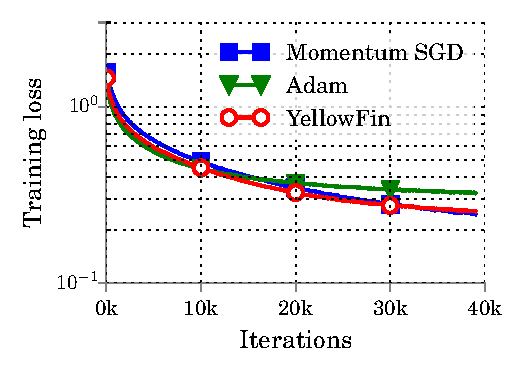
\includegraphics[width=0.4\linewidth]{experiment_results/resnet/resnet_loss.pdf} &
		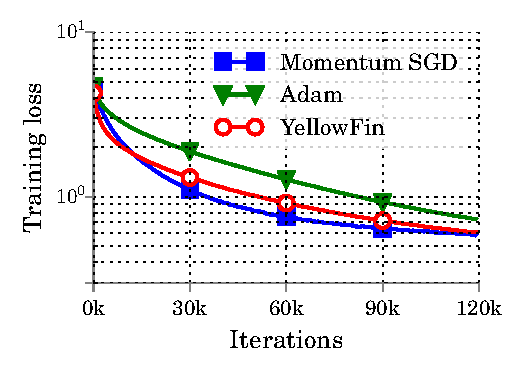
\includegraphics[width=0.4\linewidth]{experiment_results/resnet/resnet_bottleneck_loss.pdf}
	\end{tabular}
	\caption{
	Training loss for ResNet on 100-layer CIFAR10 ResNet (left) and 164-layer CIFAR100 bottleneck ResNet. }
	\label{fig:loss_result_cifar}
\end{figure}

%\subsection{Importance of momentum adaptivity}
%\label{sec:importance_momentum}
%To further emphasize the importance of momentum adaptivity in \tuner, we run YF on CIFAR100 ResNet and TS LSTM. In the experiments, \tuner tunes the learning rate. Instead of also using the momentum tuned by YF, we continuously feed prescribed momentum value $0.0$ and $0.9$ to the underlying momentum SGD optimizer which YF is tuning. In Figure~\ref{fig:cmp_fix_mom}, when comparing to \tuner with prescribed momentum 0.0 or 0.9, \tuner with adaptively tuned momentum achieves observably faster convergence on both TS LSTM and CIFAR100 ResNet. It empirically demonstrates the essential role of momentum adaptivity in \tuner.
%\begin{figure}
%\centering	
%\begin{tabular}{c c}
%	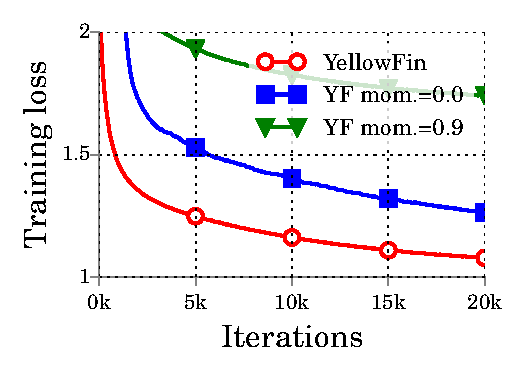
\includegraphics[width=0.4\linewidth]{experiment_results/tf_charrnn_train_loss_fix_mom.pdf} &
%	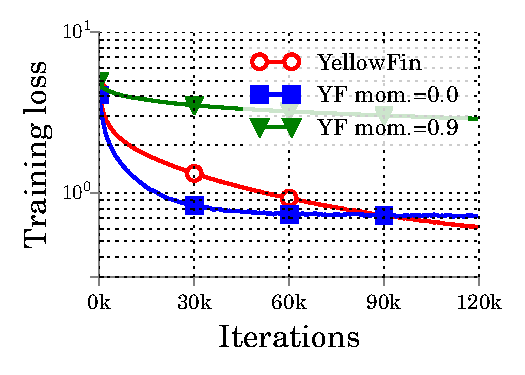
\includegraphics[width=0.4\linewidth]{experiment_results/resnet/resnet_bottleneck_loss_fix_mom_cmp.pdf}
%\end{tabular}
%\caption{Training loss comparison between \tuner with adaptive momentum and \tuner with fixed momentum value. This comparison is conducted on TS LSTM (left) and CIFAR100 ResNet (right).}
%\label{fig:cmp_fix_mom}
%\end{figure}


\subsection{Tuning momentum can improve Adam in asynchronous-parallel setting}
\begin{wrapfigure}[11]{r}{0.31\linewidth}
\vspace{-4.5em}
\begin{minipage}{1.0\linewidth}
	\begin{figure}[H]
		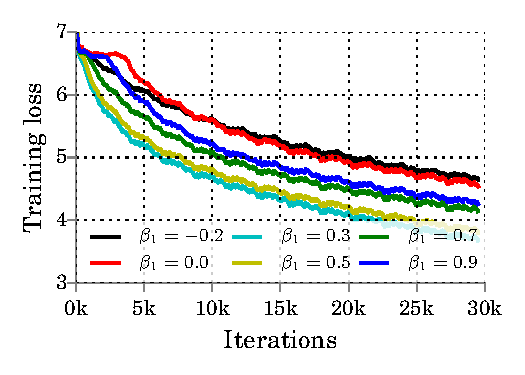
\includegraphics[width=\linewidth]{experiment_results/ptb/adam_stale_15_tuning.pdf}
			\vspace{-1.5em}
		\caption{Hand-tuning Adam's momentum under asynchrony.}
		\label{fig:adam_async_mom}
	\end{figure}
%	\vspace{-1.5em}
%	\begin{figure}[H]
%		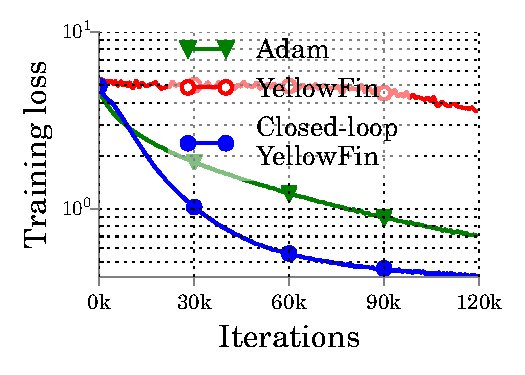
\includegraphics[width=0.975\linewidth]{experiment_results/resnet/resnet_bottleneck_cmp_tuner_adam.pdf}
%%		\caption{Adam, \tuner and \asynctuner on CIFAR100 with 16 async. workers. Sync. baseline uses \tuner.}
%	\vspace{-1.5em}
%		\caption{Asynchronous performance on CIFAR100 ResNet.}
%		\label{fig:full_async_cmp}
%	\end{figure}
\end{minipage}	
\end{wrapfigure}
%\subsection{Asynchronous experiments}
%In this section, we evaulate \tuner in an asynchronous-parallel setting,
%where we focus on {\em statistical efficiency}: the number of iterations to reach a certain solution. 
%To that end, we run $M$ asynchronous workers on a single machine and force them to update the model in a round-robin fashion,
%i.e. the staled gradient is delayed for $(M-1)$ iterations.
%We demonstrate
%%(1) Adam suffers a convergence speed penalty due to not tuning momentum in asynchronous settings;
%(1) \asynctuner (cf.\ Section~\ref{sec:async_tuner}) improves the convergence of \tuner dramatically, which leads to
%(3) \asynctuner having much faster convergence than Adam. 
%\paragraph{State-of-the-art adaptive methods suffer from lack of momentum tuning} 
We conduct experiments on PTB LSTM with 16 asynchronous workers using Adam using the same protocol as in Section~\ref{sec:async_exp}.
Fixing the learning rate to the value achieving the lowest smoothed loss in Section~\ref{subsec:sync_exp}, we sweep the smoothing parameter $\beta_1$~\citep{kingma2014adam} of the first order moment estimate in grid $\{-0.2, 0.0, 0.3, 0.5, 0.7, 0.9\}$. $\beta_1$ serves the same role as momentum in SGD and we call it the momentum in Adam. Figure~\ref{fig:adam_async_mom} shows tuning momentum for Adam under asynchrony gives measurably better training loss. 
This result emphasizes the importance of momentum tuning in asynchronous settings and suggests that state-of-the-art adaptive methods can perform sub-optimally when using prescribed momentum.

\subsection{Accelerating \tuner with finer grain learning rate tuning}
\label{sec:boost_exp}
 As an adaptive tuner, \tuner does not involve manual tuning. It can present faster development iterations on model architectures than grid search on optimizer hyperparameters. In deep learning practice for computer vision and natural language processing, after fixing the model architecture, extensive optimizer tuning (e.g. grid search or random search) can further improve the performance of a model. A natural question to ask is can we also slightly tune \tuner to accelerate convergence and improve the model performance. Specifically, we can manually multiply a positive number, the learning rate factor, to the auto-tuned learning rate in \tuner to further accelerate. 
 
In this section, we empirically demonstrate the effectiveness of learning rate factor on a 29-layer ResNext (2x64d)~\citep{xie2016aggregated} on CIFAR10 and a Tied LSTM model~\citep{press2016using} with 650 dimensions for word embedding and two hidden units layers on the PTB dataset. 
%The architecture of the models are specified in Table~\ref{tab:model_specification} in Appendix~\ref{sec:model_spec}.
 	 When running \tuner, we search for the optimal learning rate factor in grid $\{\frac{1}{3}, 0.5, 1, 2(\text{best for ResNext} ), 3 (\text{best for Tied LSTM} ), 10\}$. 
 	 Similarly, we search the same learning rate factor grid for Adam, multiplying the factor to its default learning rate $0.001$. 
 	 To further strengthen the performance of Adam as a baseline, we also run it on conventional logarithmic learning rate grid $\{5e^{-5}, 1e^{-4}, 5e^{-4}, 1e^{-3}, 5e^{-3}\}$ for ResNext and $\{1e^{-4}, 5e^{-4}, 1e^{-3}, 5e^{-3}, 1e^{-2}\}$ for Tied LSTM. We report the best metric from searching the union of learning rate factor grid and logarithmic learning rate grid as searched Adam results.
 	 Empirically, learning factor $\frac{1}{3}$ and $1.0$ works best for Adam respectively on ResNext and Tied LSTM. 
% 	 To provide another conventional baseline, we also demonstrate the performance from Adam with learning rate search on logarithmic grids. In this grid, we pick the learning rate giving the best validation/test metric. More specifically, we use grid $\{5e^{-5}, 1e^{-4}(\text{best}), 5e^{-4}, 1e^{-3}, 5e^{-3}\}$ for ResNext and $\{1e^{-4}, 5e^{-4}, 1e^{-3} (\text{best}), 5e^{-3}, 1e^{-2}\}$ for Tied LSTM. 
 	 
As shown in Figure~\ref{fig:yf_boost}, with the searched best learning rate factor, \tuner can improve validation perplexity on Tied LSTM from $88.7$ to $80.5$, an improvement of more than $9\%$. Similarly, the searched learning rate factor can improve test accuracy from $92.63$ to $94.75$ on ResNext. More importantly, we can observe, with learning rate factor search on the two models, \tuner can achieve better validation metric than the searched Adam results. It demonstrates that finer-grain learning rate tuning, i.e. the learning rate factor search, can be effectively applied on \tuner to improve the performance of deep learning models.
 	
 	
\begin{figure}
\centering
\begin{tabular}{c c} 
 	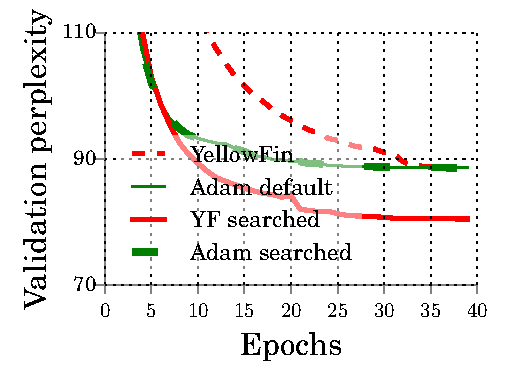
\includegraphics[width=0.4\linewidth]{experiment_results/pytorch_tied_ptb_test_perp_boost_all_seed.pdf} &
 	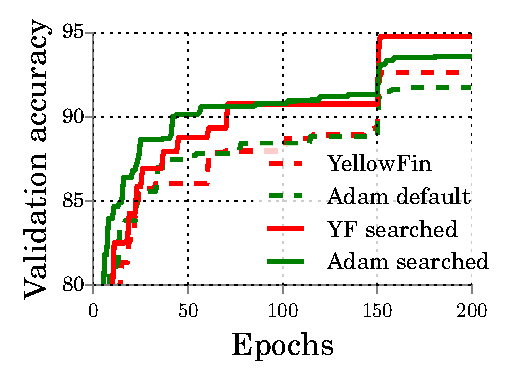
\includegraphics[width=0.4\linewidth]{experiment_results/pytorch_cifar_test_acc_boost.pdf}
\end{tabular}
\caption{Validation perplexity on Tied LSTM and validation accuracy on ResNext. Learning rate fine-tuning using grid-searched factor can further improve the performance of \tuner in Algorithm~\ref{alg:basic-algo}. \tuner with learning factor search can outperform hand-tuned Adam  on validation metrics on both models.}
\label{fig:yf_boost}
\end{figure}






%\input{test_perp}





\end{document}
